\RequirePackage{etex}
\documentclass[a4paper, 12pt, bibliography=totoc]{scrartcl}
\usepackage{notoccite}
\usepackage{iftex}
\usepackage[shortlabels]{enumitem}
\ifPDFTeX
    \usepackage[brazil]{babel}
	\usepackage[T1]{fontenc}
    \usepackage[utf8]{inputenc}
    \usepackage{cmap}
\else
	\usepackage{fontspec}
	\usepackage{polyglossia}
	\setdefaultlanguage{brazil}
	\setmonofont{DejaVu Sans Mono}[Scale=MatchLowercase]
\fi
\usepackage{indentfirst}
\usepackage{amsthm,amssymb}
\usepackage{amsmath}
\usepackage{physics}
\usepackage{algorithm}
\renewcommand{\listalgorithmname}{Lista de Algoritmos}
\usepackage[noend]{algpseudocode}
\floatname{algorithm}{Algoritmo}
\renewcommand{\algorithmicend}{\textbf{fim}}
\renewcommand{\algorithmicif}{\textbf{se}}
\renewcommand{\algorithmicthen}{\textbf{então}}
\renewcommand{\algorithmicelse}{\textbf{senão, }}
\renewcommand{\algorithmicwhile}{\textbf{enquanto}}
\renewcommand{\algorithmicdo}{\textbf{fazer}}
\renewcommand{\algorithmicreturn}{\textbf{retornar}}
\usepackage{minted}
\setmintedinline{breaklines}
\newcommand{\julia}[1]{\mintinline[breakanywhere]{julia}{#1}}
\renewcommand{\listingscaption}{Código}
\renewcommand{\listoflistingscaption}{Lista de Códigos}
\setlength{\parindent}{1cm} % padrão 15pt.
\usepackage{nomencl}
\usepackage{faktor}
\usepackage{mathtools}
\usepackage{optidef}
\usepackage{graphicx}
\usepackage{grffile} 
\usepackage{anysize}
\usepackage{cancel}
\usepackage{latexsym}
\usepackage{multicol}
\usepackage[]{mdframed}
\usepackage[colorlinks=true,urlcolor=cyan,
        pdfpagelabels=true,hypertexnames=true,
        plainpages=false,naturalnames=true]{hyperref}
%
\usepackage[shortlabels]{enumitem}
\usepackage{calrsfs}
\usepackage{dsfont}
\usepackage{siunitx}
\usepackage{booktabs}
\usepackage{threeparttable}
\usepackage[usenames,dvipsnames,svgnames,table]{xcolor}
\usepackage{xargs}
\setlength{\marginparwidth}{2cm}
\usepackage[colorinlistoftodos,prependcaption,textsize=tiny]{todonotes}
\newcommandx{\unsure}[2][1=]{\todo[linecolor=red,backgroundcolor=red!25,bordercolor=red,#1]{#2}}
\newcommandx{\change}[2][1=]{\todo[linecolor=blue,backgroundcolor=blue!25,bordercolor=blue,#1]{#2}}
\newcommandx{\info}[2][1=]{\todo[linecolor=OliveGreen,backgroundcolor=OliveGreen!25,bordercolor=OliveGreen,#1]{#2}}
\newcommandx{\improvement}[2][1=]{\todo[linecolor=Plum,backgroundcolor=Plum!25,bordercolor=Plum,#1]{#2}}
\newcommandx{\thiswillnotshow}[2][1=]{\todo[disable,#1]{#2}}
\usepackage{caption}
\usepackage{subcaption}
\usepackage[brazilian,capitalize,nameinlink,noabbrev]{cleveref}
% \creflabelformat{algorithm}{#2\textup{(#1)}#3}
\usepackage{adjustbox}
\usepackage{tabularx}
\newcolumntype{Y}{>{\centering\arraybackslash}X}
\usepackage{parnotes}
\usepackage{tikz}
\usetikzlibrary{graphs,quotes,calc}
\newcommand*\circled[1]{%
  \tikz[baseline=(C.base)]\node[draw,circle,inner sep=0.5pt](C) {#1};\!
}
\usepackage{lineno}
\usepackage{etoolbox} %% <- for \pretocmd, \apptocmd and \patchcmd
% %% Patch 'normal' math environment: (currently unused, but good to have)
\newcommand*\linenomathpatch[1]{%
  \expandafter\pretocmd\csname #1\endcsname {\linenomath}{}{}%
  \expandafter\pretocmd\csname #1*\endcsname{\linenomath}{}{}%
  \expandafter\apptocmd\csname end#1\endcsname {\endlinenomath}{}{}%
  \expandafter\apptocmd\csname end#1*\endcsname{\endlinenomath}{}{}%
}
% %% Patch AMS math environment:
\newcommand*\linenomathpatchAMS[1]{%
  \expandafter\pretocmd\csname #1\endcsname {\linenomathAMS}{}{}%
  \expandafter\pretocmd\csname #1*\endcsname{\linenomathAMS}{}{}%
  \expandafter\apptocmd\csname end#1\endcsname {\endlinenomath}{}{}%
  \expandafter\apptocmd\csname end#1*\endcsname{\endlinenomath}{}{}%
}

% Definition of \linenomathAMS depends on whether the mathlines option is provided
\expandafter\ifx\linenomath\linenomathWithnumbers
  \let\linenomathAMS\linenomathWithnumbers
  %% The following line gets rid of an extra line numbers at the bottom:
  \patchcmd\linenomathAMS{\advance\postdisplaypenalty\linenopenalty}{}{}{}
\else
  \let\linenomathAMS\linenomathNonumbers
\fi

% \linenomathpatch{equation} %% <- unnecessary, equation is already patched
\linenomathpatchAMS{gather}
\linenomathpatchAMS{multline}
\linenomathpatchAMS{align}
\linenomathpatchAMS{alignat}
\linenomathpatchAMS{flalign}
\linenomathpatchAMS{displaymath}

\usepackage{setspace}

\crefname{equation}{Equação}{Equações}
\Crefname{equation}{Equação}{Equações}

\crefalias{problem}{align}
\crefname{problem}{Problema}{Problemas}
\Crefname{problem}{Problema}{Problemas}
\creflabelformat{problem}{#2\textup{(#1)}#3}

\crefalias{method}{align}
\crefname{method}{Método}{Métodos}
\Crefname{method}{Método}{Métodos}
% \creflabelformat{method}{#2\textup{(#1)}#3}

\crefalias{ray}{equation}
\crefname{ray}{Semirreta}{Semirretas}
\Crefname{ray}{Semirreta}{Semirretas}
\creflabelformat{ray}{#2\textup{(#1)}#3}

\crefalias{constraint}{equation}
\crefname{constraint}{Restrição}{Restrições}
\Crefname{constraint}{Restrição}{Restrições}
\creflabelformat{constraint}{#2\textup{(#1)}#3}

\crefalias{constraints}{equation}
\crefname{constraints}{Restrições}{Restrições}
\Crefname{constraints}{Restrições}{Restrições}
\creflabelformat{constraints}{#2\textup{(#1)}#3}

\crefalias{expression}{equation}
\crefname{expression}{Expressão}{Expressão}
\Crefname{expression}{Expressão}{Expressão}
\creflabelformat{expression}{#2\textup{(#1)}#3}

\crefalias{code}{listing}
\crefname{code}{Código}{Códigos}
\Crefname{code}{Código}{Códigos}
\creflabelformat{code}{#2\textup{#1}#3}

\crefalias{output}{listing}
\crefname{output}{Saída}{Saídas}
\Crefname{output}{Saída}{Saídas}
\creflabelformat{output}{#2\textup{#1}#3}

\theoremstyle{plain}% default
\newtheorem{theorem}{Teorema}[section]
\newtheorem{lema}[theorem]{Lema}
\newtheorem{prop}[theorem]{Proposição}
\newtheorem{cor}[theorem]{Corolário}

\theoremstyle{definition}
\newtheorem{mydef}[theorem]{Definição}
\newtheorem{conj}[theorem]{Conjectura}
\newtheorem{fact}[theorem]{Fato}

\theoremstyle{remark}
\newtheorem{exmp}[theorem]{Exemplo}
\newtheorem{rem}[theorem]{Observação}
\newtheorem*{note}{Nota}
\newtheorem{case}{Case}
\usepackage{csquotes}
\MakeOuterQuote{"}
\usepackage[percent]{overpic}
\usepackage{systeme}
\usepackage{etoolbox}
\cslet{blx@noerroretextools}\empty
\usepackage[backend=biber,style=numeric-comp,
 maxnames=6,maxcitenames=3,isbn=false,sorting=nyt,sortcites=true,date=year]{biblatex}
\addbibresource{bibliography.bib}

\DeclareMathOperator{\aff}{aff}
\DeclareMathOperator{\circun}{circ}
\DeclareMathOperator{\s}{span}
\DeclareMathOperator{\fix}{Fix}
\def\bbm#1\ebm{\begin{bmatrix}#1\end{bmatrix}}
\def\R{\mathds{R}}
\def\Z{\mathds{Z}}
\def\N{\mathds{N}}
\def\X{\mathds{X}}
\def\Y{\mathds{Y}}
\def\vA{ A}
\def\vB{ B}
\def\vN{ N}
\def\vxB{x_B}
\def\vxN{x_N}
\def\vc{ c}
\def\vcB{c_B}
\def\vcN{c_N}
\def\vx{x}
\def\vbb{b}
\def\vbbbar{\bar{b}}
\def\ip{^\intercal}
\def\eqsys{Ax = b}
\def\objval{c\ip x}
\def\barx{\overline{x}}
\def\invB{B^{-1}}
\def\yik{y_{ik}}
\def\bi{\bar{b_i}}
\def\yrk{y_{rk}}
\def\br{\bar{b_r}}
\def\ratio{\bi/\yik}
\def\minratio{\br/\yrk}
\def\vq{q}
\def\hatinvB{\hat{B}^{-1}}
\def\vC{C}
\def\vX{X}
\def\fast{^\ast} %Flying asterisk
\def\setnozero{\backslash\{0\}}
\def\deg{^\circ}
\newcommand{\vl}[1]{L_{#1}}
\newcommand{\vBn}[1]{B_{#1}}
\newcommand{\invBn}[1]{B^{-1}_{#1}}
\newcommand{\zbar}[1]{\bar{z}_{#1}}
\newcommand{\vcc}[1]{c_{#1}}
\newcommand{\vcBn}[1]{c_{B#1}}
\newcommand{\y}[1]{y_{#1}}
\newcommand{\x}[1]{x_{#1}}
\newcommand{\bbar}[1]{\bar{b}_{#1}}
\newcommand\mc[1]{\multicolumn{1}{c}{#1}}
\newcommand\mcal[1]{\mathcal{#1}}
\DeclareMathAlphabet{\mathcal}{OMS}{cmsy}{m}{n}
\allowdisplaybreaks
\setcounter{secnumdepth}{5}
\setcounter{tocdepth}{5}
\sysdelim..
\title{Fundamentos matemáticos e computacionais de problemas de roteamento de veículos\thanks{Este trabalho foi financiado pela Propesq e PIBIC-CNPq/UFSC}}


\author{Pedro Henrique Centenaro\thanks{Acadêmico do curso de Bacharelado em Engenharia de Controle, Automação e Computação da UFSC/Campus Blumenau.} \\ Orientador: Luiz Rafael dos Santos}

\date{}
\begin{document}
% \linenumbers
\onehalfspacing
\maketitle
\renewcommand\thelinenumber{\textcolor{darkgray}{\arabic{linenumber}}}

\begin{abstract}
   \textbf{Resumo.} Este trabalho visa estabelecer os princípios matemáticos necessários ao entendimento de problemas de roteamento de veículos (PRVs), capacitados e com janelas de tempo, e os modelos propostos na literatura para resolvê-los. Como motivação, são apresentados fatos e tendências sobre urbanização e transporte público, bem como as vantagens e desafios da troca de veículos a combustão por veículos elétricos, cujas peculiaridades influenciam a modelagem dos PRVs. Abordam-se conceitos de grafos, otimização linear e inteira, bem como as implementações computacionais do método simplex e do problema do caixeiro viajante (PCV), e comparam-se os desempenhos de três \emph{solvers} e formulações do PCV. Por fim, três modelos de PRVs são apresentados e comparados.
\end{abstract}

\newpage
\tableofcontents
\newpage

\section{Introdução}
Este trabalho foi desenvolvido, de abril de 2022 a agosto de 2023, pelo discente Pedro Henrique Centenaro, estudante de Engenharia de Controle, Automação e Computação na Universidade Federal de Santa Catarina (UFSC), Campus Blumenau. O professor Luiz Rafael dos Santos atuou como orientador do projeto, e foi fornecido ao estudante acesso ao Laboratório de Matemática Aplicada e Computacional da UFSC, o LABMAC

A roteirização de veículos é um processo logístico fundamental para empresas. Entre suas aplicações, podem ser citadas a coleta de materiais recicláveis \cite{BAPTISTA:02}, coleta de lixo \cite{MARKOVIC:20}, distribuição de alimentos perecíveis \cite{AMORIM:14}, roteirização de atendimento médico \cite{ISSABAKHSH:18} e roteirização de ônibus \cite{GUO:19}. Os modelos matemáticos aplicados à resolução de tais problemas têm formulações variadas, cada qual dependendo da complexidade da análise realizada pelos autores.

O problema mais simples de roteirização é o do caixeiro viajante (PCV), em que um único veículo deve atender determinado número de pontos de modo a minimizar seus gastos com deslocamentos \cite{OR-Tools,SAIYED:12,SIQUEIRA:22}. Quando se considera uma frota, tem-se um problema de roteamento de veículos (PRV) \cite{OR-Tools-VRP}. Neste caso, é possível considerar uma quantidade muito maior de obstáculos à roteirização, como capacidades dos veículos, janelas de tempo de atendimento, múltiplos depósitos, frotas mistas e outros mais \cite{VIEIRA:13,TORO:16}.

Com o crescimento dos modelos dos problemas de roteirização, aumenta a complexidade computacional para resolvê-los. Não é incomum que se discutam soluções para PCVs relativamente pequenos que encontrem a solução ótima do problema; no entanto, para os PRVs, a prática exige que soluções quase-ótimas sejam consideradas \cite{LAPORTE:87}. Ainda assim, tanto o PCV quanto os PRVs são problemas NP-difíceis \cite{ZAMBITO:06}. Por exemplo, a resolução de um PCV de 85900 pontos necessitou do uso de 96 estações de trabalho e um poder computacional que equivale a 139 anos de funcionamento de uma única CPU \cite{BAZRAFSHAN:21}.

Tendo em vista a complexidade teórica e prática dos PRVs, o objetivo geral deste trabalho é explorar e explicar as principais características que contribuem para as dificuldades de implementação destes problemas. Já os objetivos específicos são:

\begin{itemize}
    \item Estudar as teorias dos problemas de roteamento de veículos capacitado e com janela de tempo, incluindo aplicações;
    \item Modelar PRVJT escrevendo as equações relacionadas e implementar o modelo na linguagem de modelagem JuMP;
    \item Fazer testes computacionais com diversos \emph{solvers}, em particular que utilizem técnicas exatas e heurísticas/meta-heurísticas;
    \item Reportar os resultados em formato de relatório técnico e pôster em eventos científicos.
\end{itemize}

Visando alcançar tais objetivos, os princípios matemáticos e computacionais necessários para a compreensão e implementação de modelos de roteamento foram concatenados neste relatório. A ideia é que o público-alvo seja capaz de ler o trabalho por completo, chegando ao fim com a capacidade de interpretar modelos complexos de PRVs e identificar as vantagens e desvantagens computacionais de cada tipo de formulação.

Para realizar a leitura deste documento, recomenda-se um conhecimento básico sobre demonstrações e notações matemáticas, além de álgebra linear. Na \cref{sec:urbanização e transporte público}, o transporte público urbano, seus desafios e tendências futuras são apresentados como motivadores para o estudo de PRVs. Na \cref{sec:matemática}, apresenta-se o básico de grafos, seguido de uma definição matemática formal do PCV. Pelo resto da seção, discutem-se objetos da álgebra linear necessários para compreender a ideia por trás do método simplex, muito utilizado para resolver problemas de otimização. Os mecanismos por trás deste método são discutidos em detalhes no \cref{sec:metodo_simplex}, incluindo pseudocódigo e implementação \cite{Centenaro:23} (ver o pacote \href{https://github.com/phcentenaro7/Caique.jl}{\texttt{Caique.jl}}).

A \cref{sec:considerações computacionais} lida com os aspectos computacionais de implementação e resolução de modelos. São comparados \emph{solvers}\footnote{Como é detalhado em seções posteriores, os \emph{solvers} são ferramentas computacionais robustas que tentam resolver problemas de otimização por meio de várias técnicas exatas e heurísticas.} e formulações do PCV, levando em conta a teoria desenvolvida até o momento. Detalhes de implementação podem ser encontrados no \cref{sec:PCV implementações}. Na \cref{sec:PRVJT}, são apresentados e descritos alguns modelos de PRVJTs. Similaridades e diferenças notáveis entre os modelos são comparadas, realçando o impacto que as considerações específicas de cada um têm sobre seu formato matemático e suas características computacionais. Finalmente, na \cref{sec:conclusão}, os objetivos deste trabalho são revisitados de modo a avaliar se e como foram cumpridos.
\section{Urbanização e transporte público}\label{sec:urbanização e transporte público}
O transporte público é uma necessidade ubíqua no Brasil. Particularmente nos centros urbanos, é comum que existam dificuldades na implementação e manutenção de frotas, devido à alta densidade populacional dos centros e à marginalização de setores da população, que diuturnamente precisam viajar por longos trajetos para garantirem seu sustento. Tendo em vista a grande importância deste assunto, nesta seção, são abordados fatos e tendências do transporte público, no Brasil e no mundo, que servem como inspiração para o estudo da modelagem e resolução de problemas de roteamento de veículos.

\subsection{Vantagens e tendências do transporte público}\label{sec:vantagens transporte público}

Litman \cite{LITMAN:12}, em pesquisa conduzida nos Estados Unidos, descreve vários benefícios do transporte público para seus usuários. Alguns dos mais importantes que podemos elencar são:

\begin{itemize}
    \item \textbf{Locomoção mais variada:} Quanto melhor a estrutura do transporte público de uma região, aliada à promoção de bicicletas, caminhadas e transportes alternativos, menor é o uso de automóveis particulares por parte da população. Verifica-se ainda que a média de automóveis particulares, por residência, em regiões com transporte público de alta qualidade, pode chegar a metade do que se observa em regiões com pouco investimento em transporte público.
    \item \textbf{Aumento do tempo de exercício físico:} Usuários de transporte público ou alternativo precisam andar pelo menos duas vezes mais para chegar aos seus destinos diários. Esta vantagem de tempo gasto com exercícios se mantém, visto que o tempo gasto com exercícios recreativos é aproximadamente o mesmo para usuários de transporte público ou alternativo e usuários de automóveis privados.
    \item \textbf{Declínio do número de fatalidades no trânsito:} Quando bem implementado e largamente utilizado, o transporte público incentiva mais cuidado por parte de motoristas e da legislação, pois mais pessoas passam a andar a pé ou de bicicleta. Como mostram estatísticas internacionais, comunidades em que o transporte público é bem integrado à vida das pessoas têm consideravelmente menos fatalidades no trânsito.
    \item \textbf{Redução da poluição veicular:} Ônibus elétricos e ônibus movidos a combustão mais recentes produzem cada vez menos gases nocivos, conforme evoluem as regulamentações sobre emissões. Além disso, como estes veículos podem transportar dezenas de pessoas e desincentivam o uso de veículos particulares, a poluição também é reduzida graças à redução do número de veículos nas ruas.
    \item \textbf{Integração comunitária:} Em regiões com transporte público de qualidade, a população tem acesso facilitado a serviços essenciais (saúde, educação, emprego, víveres, etc.), o que significa que as pessoas em geral terão melhores condições de saúde, mais oportunidades econômicas, menores gastos com transporte e manutenção de veículos particulares e melhores condições de saúde mental. Todas estas questões são também importantes para a administração da cidade, pois o acesso facilitado a atendimento médico permite que as pessoas se consultem antes que seus problemas de saúde se agravem. Da mesma maneira, o acesso facilitado a educação e emprego significa que mais pessoas terão acesso a maiores graus de instrução, o que pode aumentar a diversidade de profissionais do mercado da região e beneficiar a economia.
\end{itemize}

Ademais, Schwab \cite{SCHWAB:19} apresenta considerações importantes sobre as tendências de desenvolvimento das cidades. De acordo com relatório de pesquisa do Fórum Econômico Mundial \cite{FEM:15}, que ouviu 816 executivos de grandes empresas de tecnologia e inovação, a expectativa, em 2015\footnote{Talvez esta expectativa tenha sido atrasada desde então, devido à pandemia de Covid-19.}, de 64\% dos entrevistados era que até 2025 surja a primeira cidade com mais de 50 mil habitantes e sem semáforos. Diz também Schwab que

\begin{displayquote}
    \textelp{} os avanços tecnológicos de sensores, sistemas óticos, processadores embutidos, maior segurança para os pedestres e para o transporte não motorizado levarão à maior adoção do transporte público, redução dos congestionamentos e da poluição, melhor saúde e trajetos mais rápidos, mais previsíveis e menos caros.
\end{displayquote}

Schwab também argumenta que as cidades que mais rapidamente conseguirem integrar novas tecnologias aos seus espaços públicos atrairão o maior número de pessoas qualificadas para o seu desenvolvimento. Ele acrescenta:

\begin{displayquote}
    \textelp{} estudos mostram que o aumento das áreas verdes de uma cidade em 10\% poderia compensar o aumento da temperatura causado pelas mudanças climáticas \textelp{}.
\end{displayquote}

Segundo Bursztyn e Eiró \cite{BURSZTYN:15}, a preocupação com as mudanças climáticas e seus efeitos é maior entre pessoas com maior grau de escolaridade. Logo, as tecnologias verdes (particularmente, como argumentaremos, os ônibus elétricos) devem ser foco de investimento por parte das cidades que desejarem atrair estes demográficos.

Um estudo de Lima, Silva e Albuquerque Neto \cite{LIMA:19} aponta iniciativas de adoção do transporte por ônibus elétricos em cidades como Amsterdã, Cidade do Cabo, Copenhague, Hamburgo, Los Angeles, Nova Iorque, Oslo, Rugao e São Francisco. O objetivo destas cidades é substituir completamente os ônibus a combustão pelos elétricos.

Em suma, existe uma tendência entre os países mais desenvolvidos de investir nas novas tecnologias elencadas pelo Fórum Econômico Mundial \cite{FEM:15}, sendo de particular interesse para esta análise as que dizem respeito ao meio ambiente. Estas tecnologias são importantes pela redução dos impactos ambientais dos meios urbanos e pela crescente preocupação da população com seus efeitos no planeta. Como argumentamos a seguir, na \cref{sec:impactos ambientais ônibus elétricos}, é importante que as cidades brasileiras tentem seguir estas tendências adicionando ônibus elétricos a suas frotas e retirando sempre que possível os ônibus a combustão de circulação.

\subsection{Sobre ônibus elétricos}\label{sec:impactos ambientais ônibus elétricos}
Para entender os investimentos em ônibus elétricos realizados por grandes cidades, precisamos elencar seus benefícios em relação aos ônibus a combustão. O trabalho de Lima, Silva e Albuquerque Neto \cite{LIMA:19} é bastante esclarecedor a este respeito. Os autores discorrem sobre a existência de dois tipos de ônibus elétricos, os totalmente elétricos e os híbridos, apontando suas principais características. Em seguida, discutem os benefícios ambientais da implementação de tais veículos no transporte público. Por fim, os autores abordam algumas das principais dificuldades relacionadas à implementação destes veículos.

\subsubsection*{Ônibus totalmente elétricos}
Este tipo de ônibus funciona com base em baterias recarregáveis. Por este motivo, gera consideravelmente menos partículas do que modelos a combustão, além de suas emissões de gases de efeito estufa serem nulas. Um benefício de longo prazo é que este tipo de ônibus é mecanicamente mais simples, sendo mais barata a sua manutenção. Ônibus totalmente elétricos podem ser movidos por vários tipos de motores elétricos, que têm a vantagem de fornecerem maior aceleração ao veículo do que motores convencionais. Devido às suas características, ônibus totalmente elétricos têm aproximadamente três vezes a eficiência dos ônibus a combustão (59\% a 62\% de eficiência contra 17\% a 21\% de eficiência, respectivamente).

As baterias de ônibus totalmente elétricos têm um tempo de vida útil estimado entre 8 e 10 anos, podendo ser utilizadas para alimentar outros tipos de serviço após este período. Atualmente, as baterias mais utilizadas são as de íons de lítio, graças à sua eficiência. No entanto, sua reciclagem é muito custosa. É possível que no futuro estas baterias percam sua posição dominante no mercado para as de níquel-hidreto metálico, que têm grande vida útil mas, atualmente, têm alto custo e desvantagens físicas comparadas as de íons de lítio.

Uma desvantagem dos ônibus totalmente elétricos em relação aos de combustão é que o projeto dos sistemas auxiliares (como portas, direção hidráulica e compressor do ar condicionado) é mais complicado, visto que cada sistema pode precisar do seu próprio motor em configurações específicas. Desta forma, o projeto de controle individual para cada um destes motores acarreta custos adicionais com componentes, o que pode deixar estes veículos mais complexos.

\subsubsection*{Ônibus híbridos}
Ônibus híbridos misturam aspectos de ônibus totalmente elétricos com ônibus a combustão, sendo mais eficientes que os modelos a combustão e tendo a possibilidade de serem utilizados como fonte de energia para outros veículos. Ademais, seus componentes têm tamanho reduzido com o uso inteligente das baterias.

Estes veículos são hibridizados por meio de extensores de autonomia, definidos pelos autores como

\begin{displayquote}
    \textelp{} sistemas embarcados capazes de gerar energia durante a operação, recarregando as baterias e consequentemente estendendo a autonomia do veículo.
\end{displayquote}

Existem vários tipos de extensores de autonomia, sendo os principais as pilhas a combustível, grupo motor-gerador, motores a combustão interna e supercapacitores. Em geral, estes componentes permitem a recuperação ou maior eficiência energética, garantindo mais eficiência de operação. Vale prestar atenção à seguinte observação dos autores:

\begin{displayquote}
    \textelp{} em percursos com baixa necessidade de frenagens, como rodovias, as vantagens relativas à recuperação de energia diminuem a eficiência do veículo híbrido. Dessa forma, tais veículos se aproveitam melhor deste sistema em percursos com um maior número de frenagens, que é o caso do transporte urbano.
\end{displayquote}

Os veículos híbridos podem ser classificados como: em série, caso no qual são movidos por motor elétrico alimentado pelas baterias ou pelos extensores de autonomia; em paralelo, podendo ser tracionados por motor elétrico ou a combustão, juntos ou individualmente; e em série-paralelo, unindo características dos dois.

\subsubsection*{Benefícios ambientais e econômicos}
Os ônibus elétricos são muito mais eficientes do que os modelos a combustão no que se refere a emissão de substâncias nocivas ao meio-ambiente. Um problema que pode surgir com a implementação deste tipo de ônibus diz respeito ao trajeto pelo qual passa a energia até abastecê-lo. Se esta energia não for produzida de maneira limpa, pode ser enganosa a noção de que a implementação de ônibus elétricos não acarreta a produção de poluição. Felizmente, no Brasil, 74\% da energia elétrica provém de fontes limpas e renováveis. Além disso, estas fontes, em geral, ficam a grande distância da população, o que permite maior facilidade na captura de quaisquer materiais particulados que o processo de fornecimento de energia aos ônibus elétricos possa gerar, sem danos à população.

No que se refere à redução da emissão de gás carbônico, os autores observam que

\begin{displayquote}
    \textelp{} [no Brasil,] a substituição dos ônibus e micro-ônibus por modelos elétricos, considerando toda a geração de energia para carregamento desses ônibus, garantiria uma redução de 17,44 milhões de toneladas de CO$_2$ (91,4\%) para o ano de 2012.
\end{displayquote}

Quanto aos materiais particulados, os autores esclarecem que

\begin{displayquote}
    a produção de energia elétrica para alimentar a frota de micro-ônibus e ônibus urbanos elétricos emitiria 58,9\% mais material particulado do que a própria combustão do diesel \cite{LIMA:19}.
\end{displayquote}

No entanto, como já foi esclarecido, o Brasil tem as condições geográficas necessárias para lidar com estes materiais particulados eficientemente.

Os ônibus elétricos -- e os híbridos, quando operando somente com base em motor elétrico -- também ocasionam consideravelmente menos poluição sonora do que ônibus a combustão, tornando os espaços urbanos mais agradáveis e saudáveis.

Em geral, ônibus elétricos ainda requerem investimentos mais caros do que ônibus a combustão. No entanto, verifica-se que, escolhendo baterias apropriadas para a distância percorrida diariamente por cada ônibus, após atingirem determinada quilometragem, os ônibus elétricos passam a ser mais baratos do que os modelos a combustão. Além disso, as tendências internacionais indicam que os aumentos no preço do petróleo serão maiores do que no preço da eletricidade, e espera-se que os conjuntos de baterias dos ônibus elétricos se tornem consideravelmente mais baratos até 2030, ano em que ônibus elétricos devem custar tanto ou menos que ônibus a combustão\footnote{Estas expectativas são da Bloomberg New Energy Finance \cite{BLOOMBERG:18}, e foram publicadas no ano de 2018. Novamente, é importante ressaltar a possibilidade de a pandemia de Covid-19 ter afetado as expectativas.}.

\subsubsection*{Dificuldades de implementação}\label{sec:dificuldades de implementação}
Em geral, como os ônibus elétricos ainda são mais caros do que ônibus a combustão, são vistos como investimentos mais arriscados pelas operadoras de ônibus. Muitos dos ônibus elétricos adquiridos por países europeus vieram de subsídios federais, o que não constitui uma forma viável de continuar adquirindo estes veículos a longo prazo. Existe também o fato de ônibus a combustão já serem consagrados e serem impulsionados por indústrias e fabricantes já muito fortalecidos em cenários nacionais, especialmente em países em desenvolvimento.

A transição para modelos elétricos também é confrontada por problemas de padronização de infraestruturas de carregamento, apesar de haver avanços neste sentido proporcionados por acordos entre fabricantes de veículos elétricos. Existem também receios quanto à possibilidade de apagões afetarem as operações de transporte público, e há ainda a possibilidade de muitas cidades estarem esperando os preços de ônibus elétricos abaixarem antes de iniciarem seus investimentos neste tipo de tecnologia.

Apesar destas dificuldades, os benefícios dos ônibus elétricos têm peso considerável pelos motivos apresentados até aqui. Na conclusão de seu trabalho, Lima, Silva e Albuquerque Neto fazem a seguinte observação a respeito do futuro desta categoria de veículos:

\begin{displayquote}
    \textelp{} Além dos novos arranjos de financiamento, é necessário se pensar em novos desenhos de contrato com alocação de risco adequada e que garanta que o risco da tecnologia seja alocado a quem tem maior capacidade de suportá-lo. É possível que novos \emph{players} entrem no mercado de transporte urbano, como fabricantes de veículos oferecendo \emph{leasing} e manutenção dos ônibus, e \emph{utilities} de energia oferecendo infraestrutura de carregamento.
\end{displayquote}

Assim, é possível esperar que ônibus elétricos se tornem cada vez mais atraentes e viáveis conforme seu mercado se desenvolve. Feita esta análise, é importante considerar desafios especificamente brasileiros que a adesão a este tipo de veículo pode encontrar.

\subsection{O desafio do espraiamento no transporte público brasileiro}
Dados do Ipea \cite{IPEA:16} mostram que cerca de 85\% da população brasileira vive hoje em centros urbanos, sendo 36 cidades com mais de 500 mil habitantes e um restante de quarenta regiões metropolitanas que abrigam uma população total de mais de 80 milhões de habitantes. Os dados indicam que a intensa industrialização brasileira da década de 1940 em diante, que estimulou vários êxodos rurais\footnote{Por êxodo rural, entende-se o deslocamento em massa de pessoas das zonas rurais do país para centros urbanos. Por exemplo, o êxodo rural que ocorreu no Brasil entre 1950 e 1995, onde cerca de 50 milhões de habitantes realizaram tal deslocamento \cite{IPEA:00}.}, não foi acompanhada por uma urbanização de similar velocidade.

Uma consequência da urbanização mal-elaborada do Brasil é o espraiamento \cite{IPEA:10}, condição na qual os grandes centros urbanos, em vez de abrigarem todas as camadas da população, tornam-se excludentes. Os afetados por esta exclusão são os mais pobres, que precisam se estabelecer em regiões periféricas para terem onde morar. Como consequência disso, estas pessoas têm consideravelmente mais dificuldade de acesso a serviços públicos essenciais, que ficam concentrados nos centros urbanos. Como o transporte público está incluso na lista de serviços que são precarizados para estas regiões, muitas pessoas acabam recorrendo ao uso de veículos particulares, o que gera mais congestionamentos e acidentes \cite{IPEA:16}.

O aumento do número de acidentes, em particular, se deve não apenas ao aumento do número de veículos em circulação, mas às próprias características do espraiamento. Litman \cite{LITMAN:12} explica que isso se deve ao fato de os trajetos longos necessários para se chegar aos centros urbanos estimularem uma direção menos segura, com menos atenção por parte dos motoristas e mais velocidade nas pistas. Consequentemente, embora estes longos trajetos tendam a ter menos acidentes, os acidentes que acontecem tendem a ser mais graves, ou mesmo fatais. Isso contrasta com os benefícios do transporte público identificados na \cref{sec:vantagens transporte público}, um dos quais é a redução da severidade dos acidentes em centros urbanos bem-planejados, apesar de concentrarem maior número de acidentes.

\subsubsection*{O exemplo de espraiamento de Araraquara}
Borchers e Figueirôa-Ferreira \cite{BORCHERS:22} descrevem um caso de espraiamento na cidade de Araraquara, São Paulo. Em 1959, foi fundada a Companhia Troleibus Araraquara (CTA), uma companhia pública que oferecia serviço de transporte por trólebus para a população. Os trólebus eram ônibus elétricos alimentados por um sistema de cabos suspensos sobre as ruas da cidade. A princípio, a companhia tinha um centro urbano bem-delimitado para atender, sendo capaz de servir satisfatoriamente à população. No entanto, na década de 1970, começaram a surgir os primeiros grandes obstáculos ao serviço, na forma de loteamentos espraiados. Como os trólebus tinham sua mobilidade limitada por cabos, argumentou-se que seria mais difícil e custoso implementar novas linhas do serviço que atendessem os espraiamentos. Além disso, as ruas dos bairros espraiados não eram asfaltadas, o que trazia ainda mais problemas para a implementação dos trólebus. Assim, uma solução privada por ônibus a combustão apareceu na cidade, conseguindo atender as regiões mais espraiadas. Em 1999, a própria CTA abandonou os trólebus em prol de uma frota baseada totalmente em combustão, devido à maior simplicidade de atendimento às regiões espraiadas.

O objetivo deste exemplo é identificar por que o espraiamento pode acontecer. A conclusão à qual os autores chegaram, neste caso, é de que uma lógica \emph{neoliberal} afetou o desenvolvimento urbano da cidade. Os autores definem o neoliberalismo como

\begin{displayquote}
    \textelp{} uma doutrina econômico-política e filósofo-cultural que instrumentaliza de forma coercitiva e coesiva forças de acumulação por espoliação através do aparelhamento do Estado, do controle dos meios de produção -- de bens, serviços, do espaço e do próprio ser humano -- e do domínio ou subjugo de todos aqueles cuja existência serve apenas para a produção de mais-valia \textelp{}.
\end{displayquote}
Os autores definem \emph{urbanismo neoliberal} como

\begin{displayquote}
    \textelp{} a específica aplicação dessa doutrina [neoliberal] de destruição criativa no planejamento e gestão do espaço urbano, de seus habitantes e aspectos econômicos, para reconfigurar a organização territorial e assim suscitar novas formas de produção desigual do espaço urbano e acumulação de capital \textelp{}.
\end{displayquote}

Segundo o estudo, Araraquara era uma cidade marcada por grandes propriedades rurais. Com os êxodos rurais, os grandes proprietários de terras incentivaram a urbanização da região como forma de valorizar seus terrenos e, mais tarde, por um processo de especulação, vendê-los a preços mais altos. Desta forma, o centro urbano era rodeado por lotes desocupados que permaneceram nesta situação por décadas. Eventualmente, na década de 1970, o acesso à terra se tornou impossível para a população mais pobre, devido aos altos preços dos lotes em torno do centro urbano. Assim, os mais pobres tiveram que se estabelecer em terrenos mais distantes, dando início ao processo de espraiamento da cidade. Mais tarde, na década de 1980, os lotes intermediários finalmente começaram a ser ocupados, o que retardou ainda mais a possibilidade de investimentos nas regiões periféricas, já que os lotes intermediários, por estarem mais próximos do centro urbano, começaram a ser atendidos primeiro.

Como o transporte público chegou mais cedo aos terrenos mais próximos do centro urbano, isso os valorizou ainda mais, incentivando o investimento em construções verticais. Evidentemente, isso retarda ainda mais o atendimento às regiões periféricas, pois surge a necessidade de investir mais no centro urbano para atender a uma população cada vez mais densa.

Os autores argumentam que este processo não desencadeou o sucateamento do serviço de trólebus por acaso. Dizem eles que a CTA

\begin{displayquote}
    \textelp{} foi criada como uma sociedade anônima, e a composição de capital foi realizada através de uma cobrança adicional no Imposto Predial e Territorial Urbano (IPTU) \textelp{} \cite{BORCHERS:22},
\end{displayquote}
o que significa que quem financiava o serviço era a população, incluindo os moradores dos bairros espraiados, aos quais o serviço sequer chegava. Outra consequência importante deste modelo é que os maiores proprietários de terra eram também os maiores acionistas da empresa. Com o desinteresse crescente dos mais pobres em suas ações, a empresa foi ficando cada vez mais concentrada justamente nas mãos daqueles a quem menos interessava expandir o serviço da CTA para as regiões espraiadas. Com o tempo, isso levou ao fortalecimento das empresas privadas de transporte e, eventualmente, a CTA começou a dar prejuízo. Este fato foi utilizado para justificar a privatização da empresa, em 2016, além de sua concessão a um consórcio formado por duas empresas privadas.

Este exemplo mostra que o espraiamento, apesar de ser um fenômeno comum no Brasil, não é inevitável. Apesar de ser interessante modelar e analisar matematicamente este problema, o caso de Araraquara serve para instigar a seguinte pergunta: De que maneira podemos utilizar as ciências sociais para prevenir a consolidação deste tipo de fenômeno no território brasileiro? Afinal, neste caso, seria mais interessante se o fenômeno do espraiamento constituísse uma situação meramente imaginária -- se fosse apenas o delírio de um matemático aplicado, em vez de algo que se verifica na realidade. Pelo contrário, o exemplo de Araraquara nos remete ao que escreveu Sérgio Buarque de Holanda \cite{HOLANDA:20}:

\begin{displayquote}
    A democracia no Brasil foi sempre um lamentável mal-entendido. Uma aristocracia rural e semifeudal importou-a e tratou de acomodá-la, onde fosse possível, aos seus direitos ou privilégios, os mesmos privilégios que tinham sido, no Velho Mundo, o alvo da luta da burguesia contra os aristocratas.
\end{displayquote}
\include{matemática.tex}
\section{Considerações computacionais para roteirização}\label{sec:considerações computacionais}
Nesta seção, discutem-se questões computacionais de implementação e resolução de problemas de otimização linear e inteira.

\subsection{Metodologia de modelagem em ambiente computacional}
Existem centenas de linguagens de programação, como compilado por \textcite{SCHADE:23}. Excluindo linguagens puramente lúdicas, existe ainda uma vasta gama de linguagens com aplicações práticas que podem ser consideradas para uso neste trabalho, dentre as quais as mais populares são reportadas por \textcite{CARBONNELLE:23}, baseado no número de pesquisas realizadas por tutoriais de programação, fornecido pelo \emph{Google Trends}.

Costumam-se dividir linguagens de programação em duas categorias: de \emph{baixo} e \emph{alto nível}\footnote{\emph{Low-level} e \emph{high-level}, respectivamente.}. Linguagens de baixo nível são aquelas em que "as estruturas de controle e de dados refletem diretamente a arquitetura subjacente da máquina"\footnote{"\textelp{} in which the control and data structures directly reflect the underlying machine architecture."}. Em contrapartida, as linguagens de alto nível são aquelas em que estas estruturas são determinadas pelo problema a ser resolvido \cite{BUTTERFIELD:16}; ou seja, possuem maior nível de abstração.

Em 2000, \textcite{PRECHELT:00} comparou linguagens de programação divididas em três grupos:

\begin{itemize}
    \item Linguagens de alta performance: C e C++, que são de mais baixo nível do que a maioria das linguagens de programação em uso atualmente. Tratam-se de linguagens \emph{compiladas}, o que significa que seu código é transformado em código de máquina\footnote{Em essência, o código que o computador de fato utiliza para executar aplicações \cite{BUTTERFIELD:16}.} para execução. Por esta razão, são utilizadas em projetos que requeiram alta performance e uso eficiente de memória, como sistemas operacionais \cite{TORVALDS:23,WAITE:09};
    \item Linguagem intermediária: Java, separada de C e C++ pela percepção popular de que sua performance é notavelmente inferior à de C e C++ para aplicações pesadas. Java se destaca por sua robustez, tendo se popularizado pelo fato de um mesmo código funcionar em diferentes máquinas \cite{RICARTE:00};
    \item Linguagens de \emph{scripting}: Perl, Python, Rexx e Tcl, que são de mais alto nível. Destas, a que mais se destaca é Python, pela simplicidade de sua sintaxe e o grande número de bibliotecas disponíveis para os mais diversos tipos de aplicação \cite{SRINATH:17}.
\end{itemize}

O autor comparou códigos desenvolvidos por programadores nas diferentes linguagens. O objetivo era resolver um problema que envolvia carregar um grande conjunto de dados na memória e depois retornar uma saída em formato de texto pesquisando pelos dados armazenados. Prechelt concluiu que, em geral, os programas em baixo nível alcançam seus objetivos mais rapidamente. Em contrapartida, os programas em alto nível requerem menos tempo e menos linhas de código para serem implementados. Em termos de produtividade (medida em linhas de código por hora), as linguagens de programação apresentam desempenhos similares. Prechelt reconheceu a simplicidade do problema proposto e admitiu duvidar "\textelp{} que os resultados relativos para as linguagens de \emph{script} seriam tão bons aplicados a outros problemas"\footnote{"\textelp{} that the relative results for the script languages group would hold up well when applied to other problems."}.

Em artigo introduzindo a linguagem de programação Julia, os autores \textcite{JULIA} resumem esta situação:

\begin{displayquote}
    O que o programador dinâmico perde em performance, o programador em C e em Fortran perde em produtividade. Um resultado infeliz [disso] é que as áreas mais desafiadoras da computação numérica tiveram os menores benefícios com o aumento da abstração e da produtividade oferecido por linguagens de alto nível. As consequências têm sido mais sérias do que muitos percebem.\footnote{"As much as the dynamic language programmer misses out on performance, though, the C and Fortran programmer misses out on productivity. An unfortunate outcome is that the most challenging areas of numerical computing have benefited the least from the increased abstraction and productivity offered by higher-level languages. The consequences have been more serious than many realize."}
\end{displayquote}

Portanto, o objetivo da linguagem é aproximar a comunidade científica do objetivo de ter uma linguagem de alto nível e de alta performance. Os resultados apresentados por Julia para o conjunto de problemas de teste apresentado em \cite{JULIA} são comparáveis aos de implementações em C e Fortran, além de mostrarem-se mais consistente do que os das demais linguagens testadas.

Para resolver problemas de otimização em Julia, pode-se utilizar o pacote JuMP \cite{JuMP}, que permite a modelagem de problemas de vários tipos. Seu grande diferencial é que o pacote atua como um intermediário entre o programador e o \emph{solver}, que é a ferramenta utilizada para de fato resolver os problemas. A forma como se adicionam restrições a um problema de otimização, por exemplo, são radicalmente diferentes entre os \emph{solvers} Gurobi \cite{GUROBI:22} e GLPK \cite{GLPK}, de modo que a comparação entre \emph{solvers} se torna um processo muito trabalhoso, mesmo para modelos pequenos. O JuMP resolve este problema com uma forma unificada de modelar problemas, podendo traduzi-los automaticamente de \emph{solver} para \emph{solver}.

\begin{exmp}

Considere o problema de otimização extraído de \cite{FERRIS:07}:
\begin{customopti}|s|
  {max}{}{2x_{1}+3x_{2}}{}{}
  \addConstraint{-4x_{1}+3x_{2}}{\leq12}
  \addConstraint{2x_{1}+x_{2}}{\leq6}
  \addConstraint{x_{1}+x_{2}}{\geq3}
  \addConstraint{5x_{1}+x_{2}}{\geq4}
  \addConstraint{x_{1},x_{2}}{\geq0}.
\end{customopti}

Este problema pode ser modelado em JuMP conforme o \cref{cod:ex362jump}.

\begin{listing}[H]
\centering
\inputminted[mathescape,
               linenos,
               numbersep=5pt,
            %   frame=lines,
            % framesep=2mm
            ]{julia}{códigos/ex362jump.jl}
\caption{Código em Julia do exemplo 3-6-2 usando o \texttt{JuMP.jl}.}
\label[code]{cod:ex362jump}
\end{listing}

A linha \julia{lp = Model(GLPK.Optimizer)} especifica que o \emph{solver} desejado é o GLPK. Se, por exemplo, for desejável alterar o \emph{solver} para o Gurobi, é possível fazê-lo com \julia{set_optimizer(lp, Gurobi.Optimizer)}. A chamada \julia{optimize!(lp)} solicita que o \emph{solver} escolhido resolva o problema. A \cref{cod:output362jump} confirma que a resolução foi bem-sucedida.

\begin{listing}[H]
\centering
\floatname{listing}{Saída}
\inputminted[mathescape,
               linenos,
               numbersep=5pt,
            %   frame=lines,
            % framesep=2mm
            ]{text}{códigos/output362jump.txt}
\caption{Saída do exemplo 3-6-2 usando o \texttt{JuMP.jl}.}
\label[output]{cod:output362jump}
\end{listing}

\end{exmp}

Por todas as razões apresentadas, escolheu-se o Julia para implementar todos os códigos deste trabalho.

\subsection{Técnicas de otimização inteira}
Problemas de otimização inteira são de difícil resolução. É necessário utilizar ferramentas capazes de misturar diversas técnicas para resolvê-los. Tais ferramentas são conhecidas como \emph{solvers}\footnote{Uma tradução literal seria "resolvedor".}.

\subsubsection{Técnicas exatas}
Em geral, os \emph{solvers} tentam resolver problemas de otimização inteira utilizando técnicas exatas de resolução. Estas técnicas são preferíveis por conduzirem o problema à solução ótima de fato. Em contrapartida, sua aplicação costuma tornar a resolução dos problemas mais lenta. O contrário de tais técnicas são as \emph{heurísticas} e \emph{meta-heurísticas}, abordadas adiante.

Geralmente, técnicas exatas envolvem resolver versões relaxadas dos problemas de otimização. Em seguida, verifica-se a factibilidade da resolução relaxada e, se necessário, dividem-se os problemas em problemas menores. Repete-se este processo iterativamente até obter-se uma solução que satisfaça as restrições inteiras e seja ótima.

\textcite{BRADLEY:77,MOHAMED:21} comparam problemas de otimização inteira com suas versões relaxadas. É um erro assumir que a solução inteira ótima para um problema pode ser encontrada arredondando-se ou truncando-se o valor do caso relaxado. Isso se deve a dois motivos: a possibilidade de o valor obtido não ser factível e o fato de a solução inteira poder estar radicalmente distante da linear. Para resolver problemas assim, estes autores introduzem a técnica de \emph{branch-and-bound}, resumida a seguir:

\begin{enumerate}[(a)]
    \item Resolve-se a versão relaxada da formulação inicial do problema, $P_0$. Para-se se nenhuma restrição inteira for violada;
    \item Escolhe-se uma variável $x$ que deveria ser inteira, mas tem valor $x = \alpha \notin \mathbb{Z}$, e criam-se dois novos problemas lineares: $P_1$, com restrição $x \leq \lfloor\alpha\rfloor$, e $P_2$, com restrição $x \geq \lceil\alpha\rceil$;
    \item Resolve-se um dos problemas não resolvidos. Se a solução não for a ótima, repete-se (b). Do contrário, para-se.
\end{enumerate}

O resultado deste procedimento é a criação de uma árvore, em que cada nó é um problema e cada folha é um problema a resolver \cite{GUROBI:22}. A decisão sobre qual folha explorar e a estratégia usada para determinar mais rapidamente uma solução ótima dependem da implementação do \emph{solver} \cite{CLAUSEN:99}.

Uma técnica mais robusta é o \emph{branch-and-cut}. Esta ténica amplia o \emph{branch-and-bound} por meio de \emph{planos de corte}, que são restrições que reduzem o tamanho do poliedro do problema sem excluir soluções inteiras \cite{CARRANO:19}. Quanto maior o número de soluções inteiras em que a restrição for ativa, melhor será o plano de corte. Como o poliedro resultante é menor do que o original, é provável que sejam necessárias menos iterações de \emph{branch-and-bound} para resolver o problema.

Um exemplo de plano de corte é o de Gomory. Suponha que a $i$-ésima restrição linear de um problema com $n$ variáveis de decisão seja $\sum_{j = 1}^{n}a_{ij}x_{j} = b_i$. Então, o seu plano de corte de Gomory será a restrição original menos a restrição com todas as constantes arredondadas para baixo \cite{LEUNG:12,RAVELO:20}:

\begin{equation}
    \sum_{j = 1}^{n}(a_{ij} - \lfloor a_{ij} \rfloor) x_{i} \leq b_i - \lfloor b_i \rfloor.
\end{equation}

Métodos ainda mais robustos podem ser utilizados em busca de soluções exatas. Um exemplo é o \emph{branch-and-price}, que adiciona a técnica de geração de colunas ao \emph{branch-and-bound} e envolve resolver um problema principal e um subproblema, que espera-se que reduza o caminho trilhado para se obter a melhor solução. Este método pode ser combinado com o \emph{branch-and-cut}, formando o que é conhecido como \emph{branch-and-cut-and-price} \cite{CHALAWSKY:22,VIEIRA:13}.

\subsubsection{Técnicas heurísticas}\label{sec:técnicas heurísticas}
Heurísticas são métodos aplicados a problemas específicos que podem gerar atalhos em direção à solução ótima. Estes métodos não têm o rigor matemático de algoritmos e, portanto, não existe a garantia de que sua aplicação será eficiente \cite{BUTTERFIELD:16,VIEIRA:13}.

Um exemplo de heurística para resolução do PCV é apresentado por \textcite{SCHERMER:23}. O procedimento é resumido a seguir.

\begin{enumerate}[(a)]
    \item Dado um PCV assimétrico com grafo $G = (\mcal{V}, \mcal{A})$, em que $\mcal{V}$ é o conjunto de vértices e $\mcal{A}$ é o conjunto de arestas do problema, gerar o seguinte modelo:
        \begin{align}
            \min& \sum_{i,j \in \mcal{V}}{x_{ij}c_{ij}}&&\\
            \text{s.a }& \sum_{j \in \mcal{V}}x_{ij} = 1,&\forall i \in \mcal{V},\ i \neq j,&\\
            &            \sum_{i \in \mcal{V}}x_{ij} = 1,&\forall j \in \mcal{V},\ j \neq i,&\\
            &            x_{ii} = 0,&\forall i \in \mcal{V},&\\
            &            x_{ij} \in \{0, 1\},&\forall i, j \in \mcal{V};
        \end{align}
    \item Solicitar que o \emph{solver} resolva o modelo atual do problema;
    \item Procurar pelo menor ciclo na solução gerada pelo \emph{solver}, com conjunto $S\fast$ de vértices, e parar se $S\fast = \mcal{V}$;
    \item Adicionar a restrição $\sum_{i,j \in S\fast}x_{ij} \leq |S\fast| - 1, \forall S\fast\subsetneq \mcal{V}$ ao modelo. Voltar para (b).
\end{enumerate}

Segundo Schermer, ``prevenir apenas o menor ciclo geralmente é o suficiente para quebrar outros subciclos e mantém o modelo pequeno''.\footnote{"\textelp{} preventing just the shortest cycle is often sufficient for breaking other subtours and will keep the model size smaller."} Duas maneiras são apresentadas para implementar esta heurística:

\begin{itemize}
    \item Iterativa: Espera-se que o \emph{solver} finalize sua resolução do problema para procurar pelo menor subciclo gerado. Então, gera-se um novo modelo e solicita-se que o \emph{solver} o resolva desde o início;
    \item Com \emph{lazy constraints}\footnote{Literalmente, "restrições preguiçosas". Estas restrições recebem este nome por passarem a atuar no problema apenas a partir do momento em que são violadas.}: Inclui-se no modelo uma função de \emph{callback}\footnote{Uma função $f$ é função de \emph{callback} quando é passada como argumento para uma função $F$, que, em algum momento, chama $f$ durante sua execução.} que recebe atualizações de \emph{status} do \emph{solver}. Sempre que o \emph{solver} encontra uma solução inteira ótima para o modelo fornecido, esta função procura pelo menor subciclo e o introduz dinamicamente no modelo.
\end{itemize}

Espera-se que o método de \emph{lazy constraints} seja mais eficiente, pois o \emph{solver} retém as informações obtidas sobre o modelo até o momento. Curiosamente, Schermer observou o contrário no teste que realizou para seu modelo de exemplo, demonstrando a natureza probabilística da aplicação de heurísticas ao problema.

Para PRVs, heurísticas mais robustas são necessárias, pois as violações de restrições não são tão óbvias quanto ciclos não-hamiltonianos. Um exemplo é o problema capacitado, que envolve otimizar o trajeto de uma frota de veículos com capacidade máxima de entregas para cada veículo. Além de procurar por ciclos que não incluem o depósito, \textcite{ACHUTHAN:96} propõem uma heurística que faz três pesquisas em subconjuntos de vértices. A primeira procura por violações a restrições dentro de ciclos envolvendo o depósito, a segunda procura por violações fora de cada ciclo e a terceira faz uma checagem final de todos os ciclos para os quais não foram encontradas restrições.

% \begin{align}
%     \text{min\ } &\sum_{i > j}c_{ij}x_{ij}&&\\
%     \text{s.a\ } &\sum_{i \in \mcal{V}\fast}x_{nj} = 2V,&&\\
%     &\sum_{i>k}x_{ik} + \sum_{k>i}x_{ki} = 2,&\forall k \in \mcal{V}\fast,&\\
%     &\sum_{\substack{i,j \in S\\i>j}x_{ij}} \leq |S| - \ell(S),&\forall S \subseteq\mcal{V}\fast, 3 \leq |S| \leq n - 2,&\\
%     &x_{ij} = \begin{cases}
%         \text{0, 1 ou 2 para i = n},\\
%         \text{0 ou 1, do contrário},
%     \end{cases}&&\\
%     &V > 0.&&
% \end{align}

% Nesta formulação, a matriz de adjacência é triangular inferior, sendo utilizados apenas os elementos $x_{ij}$ com $i > j$.

Existem técnicas mais gerais, conhecidas como meta-heurísticas, que podem ser aplicadas a diferentes tipos de problemas e conseguem evitar alguns dos obstáculos enfrentados pelas heurísticas. Exemplos populares já utilizados para resolver PRVs incluem a busca tabu, a colônia de formigas e os algoritmos evolucionários \cite{VIEIRA:13}.

\subsection{Comparações computacionais}
Nesta seção, apresenta-se um método para comparar \emph{solvers} e formulações de roteirização.

\subsubsection{Comparação de formulações}
O objetivo desta seção é demonstrar uma possível comparação de formulações de problemas. Toma-se como base o PCV, devido à maior simplicidade de implementação. No entanto, esta comparação também pode ser feita para diferentes formulações de VRPs.

Em 2021, \textcite{BAZRAFSHAN:21} compararam as três formulações de PCV apresentadas na \cref{sec:PCV}. Os autores analisaram os desempenhos das formulações para 10 problemas diferentes, de 10 a 500 pontos, com coordenadas aleatórias para os vértices. Das três formulações, os autores constataram que a GG é a melhor, seguida pela MTZ. A partir de 19 pontos, a formulação DFJ sequer consegue resolver problemas no tempo limite.

A família de restrições da DFJ é imposta sobre todos os subconjuntos próprios do problema, exceto pelo conjunto vazio. Isso significa que o número de restrições desta família é $|2^\mcal{V}| - 2$, sendo $2^\mcal{V}$ o conjunto potência do conjunto de vértices do problema, $\mcal{V}$. Este crescimento exponencial sobrecarrega o \emph{solver} logo no início da resolução do problema, inviabilizando-a.

Para resolver os problemas relaxados, a formulação MTZ leva vantagem sobre a GG, por adicionar menos variáveis e restrições ao problema. Ainda assim, os autores consideram a GG melhor, pois suas variáveis de ordenação são reais, ao passo que as da MTZ são inteiras. Como resultado, a MTZ tem desempenho inferior quando o modelo é passado da forma relaxada para a forma inteira.

Em relação às formulações do PCV, esta seção tem dois objetivos: verificar se as conclusões de \textcite{BAZRAFSHAN:21} sobre as formulações GG e MTZ se confirmam e comparar estas formulações à DFJ com a técnica de \emph{lazy constraints} apresentada na \cref{sec:técnicas heurísticas}. Para tal, foram criados 3 conjuntos com 10 problemas gerados aleatoriamente em cada um. Os problemas do conjunto A têm 10 pontos; do B, têm 15; e do C têm 20. Em seguida, os problemas foram resolvidos por três \emph{solvers}: GLPK \cite{GLPK}, CPLEX \cite{CPLEX} e Gurobi \cite{GUROBI:22}. Para estes testes, foi utilizado um \emph{IdeaPad} com processador Intel Core i5-10210U, 1.60 GHz, memória de 8 GB e suporte a até 8 \emph{threads}. Os tempos de resolução foram fornecidos pelos próprios \emph{solvers}, gerando a \cref{tab:tempos pcv}. As implementações são fornecidas no \cref{sec:PCV implementações}.

\begin{table}
\centering
\caption{Tempos (s) de resolução para diferentes \emph{solvers} e formulações.}\label{tab:tempos pcv}
\begin{threeparttable}
\begin{tabular}{lccccccccc}
\toprule
& \multicolumn{3}{c}{GLPK} & \multicolumn{3}{c}{CPLEX} & \multicolumn{3}{c}{Gurobi}
\\\cmidrule(lr){2-4}\cmidrule(lr){5-7}\cmidrule(lr){8-10}
           & DFJ* & MTZ & GG & DFJ* & MTZ & GG & DFJ* & MTZ & GG\\\midrule
A1 & $2.964$ & $0.746$ & $\mathbf{0.055}$ & $0.703$ & $0.461$ & $\mathbf{0.046}$ & $0.641$ & $0.333$ & $\mathbf{0.022}$\\
A2 & $\mathbf{0.002}$ & $0.228$ & $0.056$ & $\mathbf{0.008}$ & $0.118$ & $0.050$ & $\mathbf{0.008}$ & $0.191$ & $0.021$\\
A3 & $\mathbf{0.003}$ & $0.087$ & $0.036$ & $\mathbf{0.011}$ & $0.077$ & $0.066$ & $\mathbf{0.006}$ & $0.116$ & $0.016$\\
A4 & $\mathbf{0.002}$ & $0.016$ & $0.035$ & $\mathbf{0.005}$ & $0.026$ & $0.025$ & $\mathbf{0.003}$ & $0.060$ & $0.035$\\
A5 & $\mathbf{0.002}$ & $0.220$ & $0.217$ & $\mathbf{0.005}$ & $0.093$ & $0.039$ & $\mathbf{0.008}$ & $0.149$ & $0.017$\\
A6 & $\mathbf{0.002}$ & $0.032$ & $0.017$ & $\mathbf{0.008}$ & $0.031$ & $0.015$ & $\mathbf{0.006}$ & $0.043$ & $0.015$\\
A7 & $\mathbf{0.007}$ & -- & $0.057$ & $\mathbf{0.012}$ & $0.078$ & $0.044$ & $\mathbf{0.008}$ & $0.085$ & $0.035$\\
A8 & $\mathbf{0.002}$ & $1.188$ & $0.177$ & $\mathbf{0.005}$ & $1.356$ & $0.140$ & $\mathbf{0.004}$ & $0.488$ & $0.059$\\
A9 & $\mathbf{0.004}$ & $0.074$ & $0.089$ & $\mathbf{0.007}$ & $0.031$ & $0.036$ & $\mathbf{0.009}$ & $0.091$ & $0.021$\\
A10 & $\mathbf{0.003}$ & $0.210$ & $0.112$ & $\mathbf{0.013}$ & $0.049$ & $0.057$ & $\mathbf{0.007}$ & $0.178$ & $0.031$\\
B1 & $\mathbf{0.048}$ & $3.341$ & -- & $\mathbf{0.035}$ & $0.354$ & $0.514$ & $\mathbf{0.038}$ & $0.274$ & $0.208$\\
B2 & $\mathbf{0.015}$ & $1.412$ & $1.047$ & $\mathbf{0.061}$ & $0.139$ & $0.377$ & $\mathbf{0.044}$ & $0.371$ & $0.159$\\
B3 & $\mathbf{0.053}$ & -- & $18.238$ & $\mathbf{0.035}$ & $0.215$ & $0.183$ & $\mathbf{0.025}$ & $0.225$ & $0.078$\\
B4 & $\mathbf{0.028}$ & $47.536$ & $0.861$ & $\mathbf{0.037}$ & $18.583$ & $0.218$ & $\mathbf{0.019}$ & $3.612$ & $0.091$\\
B5 & $\mathbf{0.022}$ & $1.244$ & $0.462$ & $\mathbf{0.018}$ & $0.338$ & $0.114$ & $\mathbf{0.019}$ & $0.293$ & $0.063$\\
B6 & $\mathbf{0.006}$ & $0.274$ & $3.103$ & $\mathbf{0.036}$ & $0.074$ & $0.098$ & $\mathbf{0.026}$ & $0.140$ & $0.069$\\
B7 & $\mathbf{0.008}$ & -- & $3.711$ & $\mathbf{0.028}$ & $0.332$ & $0.138$ & $\mathbf{0.012}$ & $0.261$ & $0.134$\\
B8 & $\mathbf{0.022}$ & $2.148$ & $3.205$ & $\mathbf{0.016}$ & $0.540$ & $0.276$ & $\mathbf{0.012}$ & $0.364$ & $0.107$\\
B9 & $\mathbf{0.010}$ & -- & $18.597$ & $\mathbf{0.016}$ & $0.091$ & $0.087$ & $\mathbf{0.011}$ & $0.119$ & $0.063$\\
B10 & $\mathbf{0.019}$ & -- & $43.736$ & $\mathbf{0.036}$ & $18.869$ & $0.192$ & $\mathbf{0.019}$ & $2.609$ & $0.094$\\
C1 & $\mathbf{0.022}$ & -- & -- & $\mathbf{0.061}$ & $2.832$ & $0.127$ & $\mathbf{0.055}$ & $1.485$ & $0.304$\\
C2 & $\mathbf{0.064}$ & $9.668$ & $8.949$ & $\mathbf{0.149}$ & $0.408$ & $0.372$ & $\mathbf{0.046}$ & $1.434$ & $0.135$\\
C3 & $\mathbf{0.012}$ & $11.405$ & -- & $\mathbf{0.026}$ & $0.484$ & $0.501$ & $\mathbf{0.026}$ & $0.372$ & $0.150$\\
C4 & $\mathbf{0.226}$ & -- & -- & $\mathbf{0.116}$ & $8.615$ & $0.428$ & $\mathbf{0.054}$ & $2.957$ & $0.229$\\
C5 & $\mathbf{0.035}$ & $27.043$ & $22.634$ & $\mathbf{0.040}$ & $8.298$ & $0.138$ & $\mathbf{0.021}$ & $3.103$ & $0.241$\\
C6 & $\mathbf{0.023}$ & -- & -- & $\mathbf{0.085}$ & $0.732$ & $1.192$ & $\mathbf{0.059}$ & $1.670$ & $0.234$\\
C7 & $\mathbf{0.160}$ & $13.547$ & -- & $\mathbf{0.049}$ & $1.304$ & $0.531$ & $\mathbf{0.046}$ & $0.918$ & $0.271$\\
C8 & $\mathbf{0.089}$ & -- & $18.351$ & $\mathbf{0.137}$ & $7.881$ & $0.468$ & $\mathbf{0.056}$ & $4.076$ & $0.289$\\
C9 & $\mathbf{0.138}$ & $31.818$ & -- & $\mathbf{0.075}$ & $4.832$ & $0.225$ & $\mathbf{0.052}$ & $2.992$ & $0.130$\\
C10 & $\mathbf{0.074}$ & $1.840$ & -- & $\mathbf{0.057}$ & $0.117$ & $0.271$ & $\mathbf{0.024}$ & $0.244$ & $0.110$\\
\bottomrule
\end{tabular}
\begin{tablenotes}
\item A, conjuntos de 10 pontos; B, conjuntos de 15 pontos; C, conjuntos de 20 pontos; DFJ*, DFJ com \emph{lazy constraints}. Tempos maiores do que 60 s foram desconsiderados e substituídos por travessão.
\end{tablenotes}
\end{threeparttable}
\end{table}

Constata-se que a formulação GG de fato é superior à MTZ para a resolução completa do PCV. Ademais, a formulação DFJ com \emph{lazy constraints} consegue chegar à resposta ótima mais rapidamente do que as demais em todos os testes exceto um. Talvez esta anomalia possa ser explicada por se tratar do primeiro teste realizado com cada \emph{solver}. É possível que os \emph{solvers} contabilizem algum tempo de inicialização adicional nesta situação.

\subsubsection{Comparação de solvers}
Para comparar os \emph{solvers}, utilizou-se a metodologia de Dolan e Moré \cite{DOLAN:02}. Sejam $\mathcal{P}$ e $\mathcal{S}$ conjuntos de problemas e \emph{solvers}, respectivamente. Para todo problema $p \in \mathcal{P}$ e \emph{solver} $s \in \mathcal{S}$, obtém-se uma performance $t_{p,s}$ de acordo com alguma métrica de desempenho (tempo de resolução, número de funções utilizadas, etc.). Então, obtêm-se as razões entre os desempenhos de cada \emph{solver} e o desempenho do melhor \emph{solver} para determinado problema:

\begin{equation}
    r_{p,s} = \frac{t_{p,s}}{\min\{t_{p,s} \mid s \in \mathcal{S}\}}.
\end{equation}

Então, define-se uma função estatística chamada de \emph{performance profile}\footnote{"Perfil de performance."}, que representa uma distribuição das probabilidades de um problema $p \in \mcal{P}$ ser resolvido por um \emph{solver} $s \in \mcal{S}$ dentro de um intervalo $[1,\tau]$ de razões em relação ao resultado do melhor \emph{solver} para o problema em questão:

\begin{equation}
    \rho_s(\tau) = \frac{1}{|\mathcal{P}|}|\{p \in \mathcal{P}\ \mid r_{p,s} \leq \tau\}|.
\end{equation}

Aplicando este procedimento aos resultados da \cref{tab:tempos pcv}, obtêm-se as \cref{fig:pgraph10,fig:pgraph15,fig:pgraph20}, onde são comparados os \emph{performance profiles} dos três \emph{solvers} testados, tomando o DFJ com \emph{lazy constraints} como base.

\begin{figure}
    \centering
    \caption{\emph{Performance profiles} para o conjunto de 10 pontos}
    \label{fig:pgraph10}
    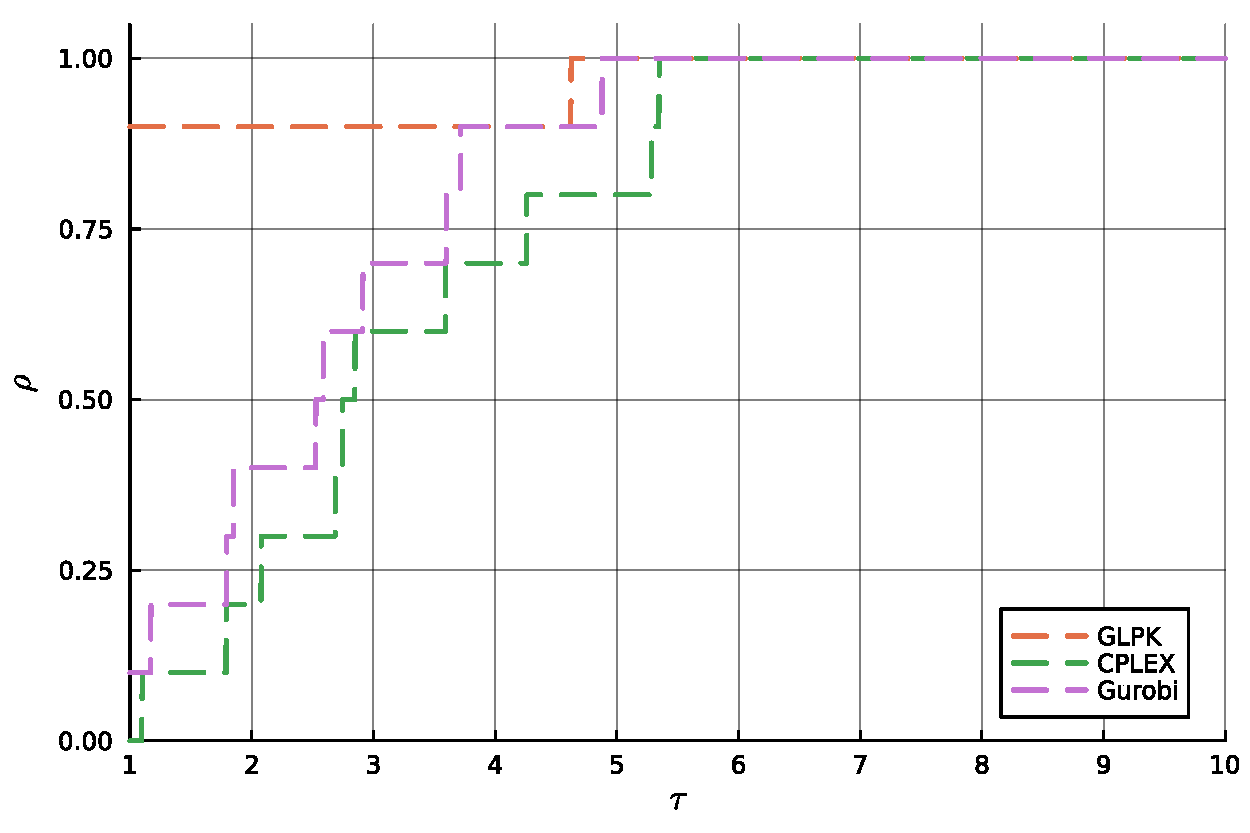
\includegraphics[scale=0.6]{imagens/pgraph10.pdf}
\end{figure}
\begin{figure}
    \centering
    \caption{\emph{Performance profiles} para o conjunto de 15 pontos}
    \label{fig:pgraph15}
    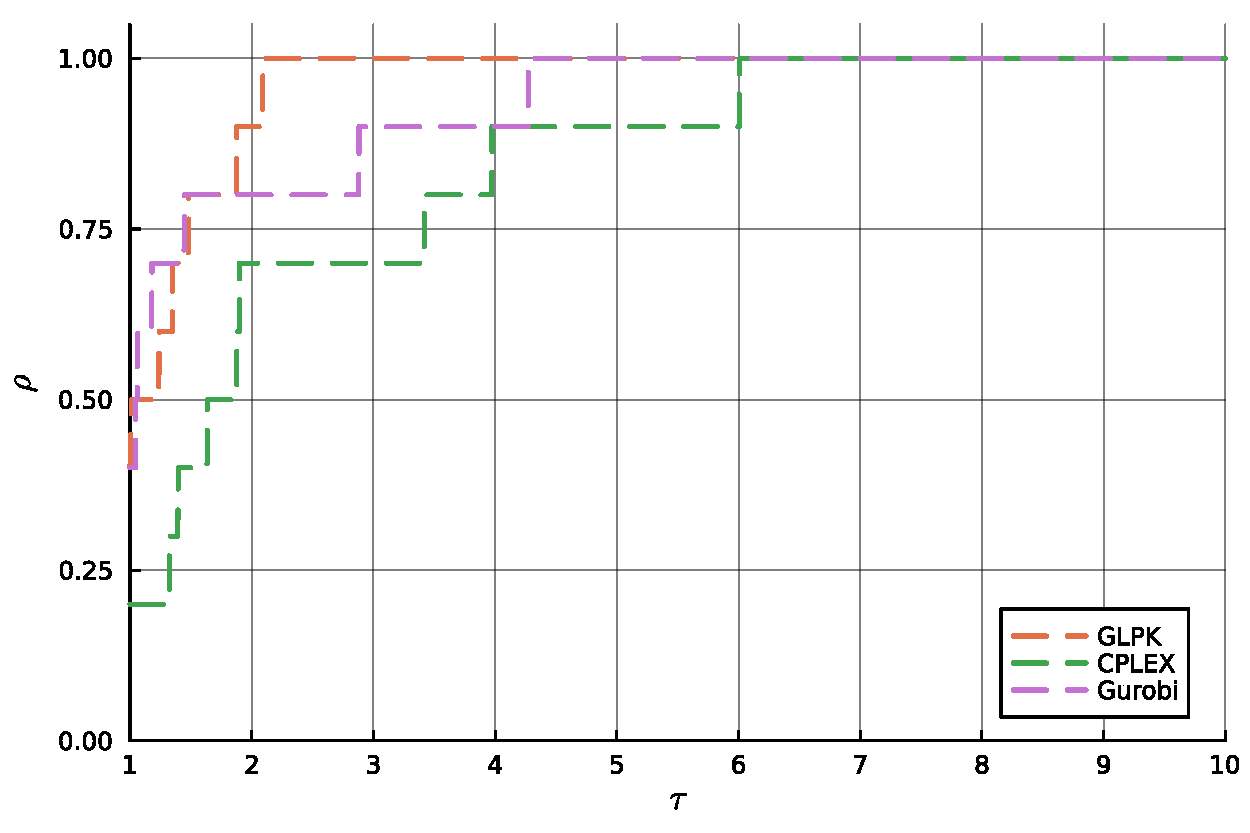
\includegraphics[scale=0.6]{imagens/pgraph15.pdf}
\end{figure}
\begin{figure}
    \centering
    \caption{\emph{Performance profiles} para o conjunto de 20 pontos}
    \label{fig:pgraph20}
    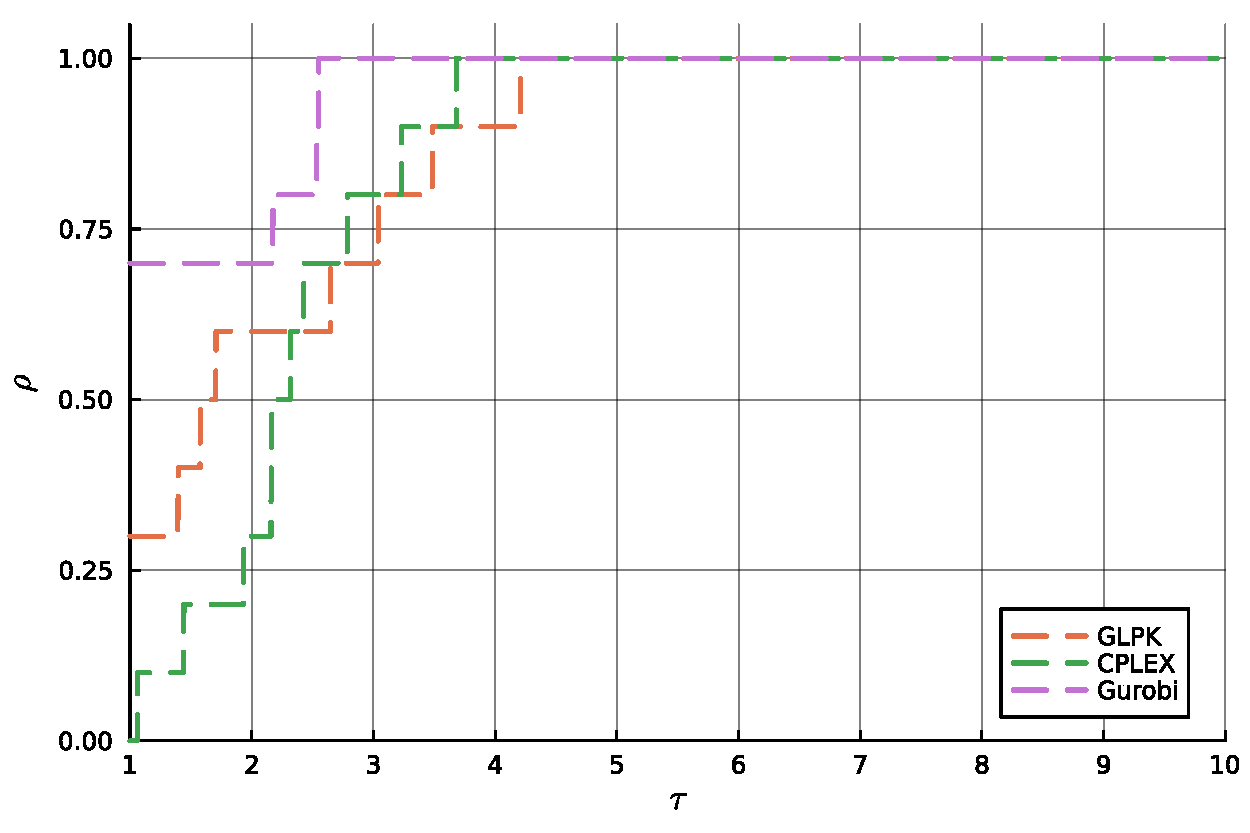
\includegraphics[scale=0.6]{imagens/pgraph20.pdf}
\end{figure}

Cada "degrau" num gráfico de \emph{performance profiles} indica a razão de problemas resolvidos no tempo relativo indicado pelas abscissas. Assim, o \emph{solver} cujo \emph{performance profile} intercepta as ordenadas com valor mais alto é o que chega à solução ótima mais rapidamente na maioria dos casos. Para 10 pontos, o GLPK é dominante neste aspecto. O Gurobi passa a dominar conforme o número de pontos aumenta.

Com 20 pontos, o Gurobi começa a se distanciar dos demais \emph{solvers}. O GLPK e o CPLEX apresentam desempenhos similares. Realizou-se mais um teste, este com 10 problemas de 50 pontos, para verificar a tendência de desempenho dos \emph{solvers} em situações mais extremas. Os resultados são apresentados na \cref{tab:tempos pcv50}.

\begin{table}
\centering
\caption{Tempos (s) de resolução para PCVs de 50 pontos usando DFJ com \emph{lazy constraints}}\label{tab:tempos pcv50}
\begin{threeparttable}
\begin{tabular}{lccc}
\toprule
GLPK & CPLEX & Gurobi\\\midrule
-- & $1.530$ & $\mathbf{0.983}$\\
$13.778$ & $\mathbf{0.312}$ & $0.395$\\
-- & $0.652$ & $\mathbf{0.535}$\\
-- & $\mathbf{0.365}$ & $0.451$\\
-- & $0.598$ & $\mathbf{0.517}$\\
-- & $0.918$ & $\mathbf{0.440}$\\
-- & $0.511$ & $\mathbf{0.381}$\\
-- & $1.523$ & $\mathbf{0.702}$\\
-- & $1.071$ & $\mathbf{0.630}$\\
$35.082$ & $0.747$ & $\mathbf{0.410}$\\
\bottomrule
\end{tabular}
\begin{tablenotes}
\item Tempos maiores do que 60 s foram substituídos por travessão.
\end{tablenotes}
\end{threeparttable}
\end{table}

A \cref{fig:pgraph50} mostra uma comparação dos \emph{performance profiles} para 50 pontos, desconsiderando o GLPK. Verifica-se que o Gurobi continua à frente, apesar de o CPLEX conseguir uma performance comparável, sendo pouco mais que duas vezes mais lento no pior dos casos.

\begin{figure}
    \centering
    \caption{\emph{Performance profiles} para o conjunto de 50 pontos}\label{fig:pgraph50}
    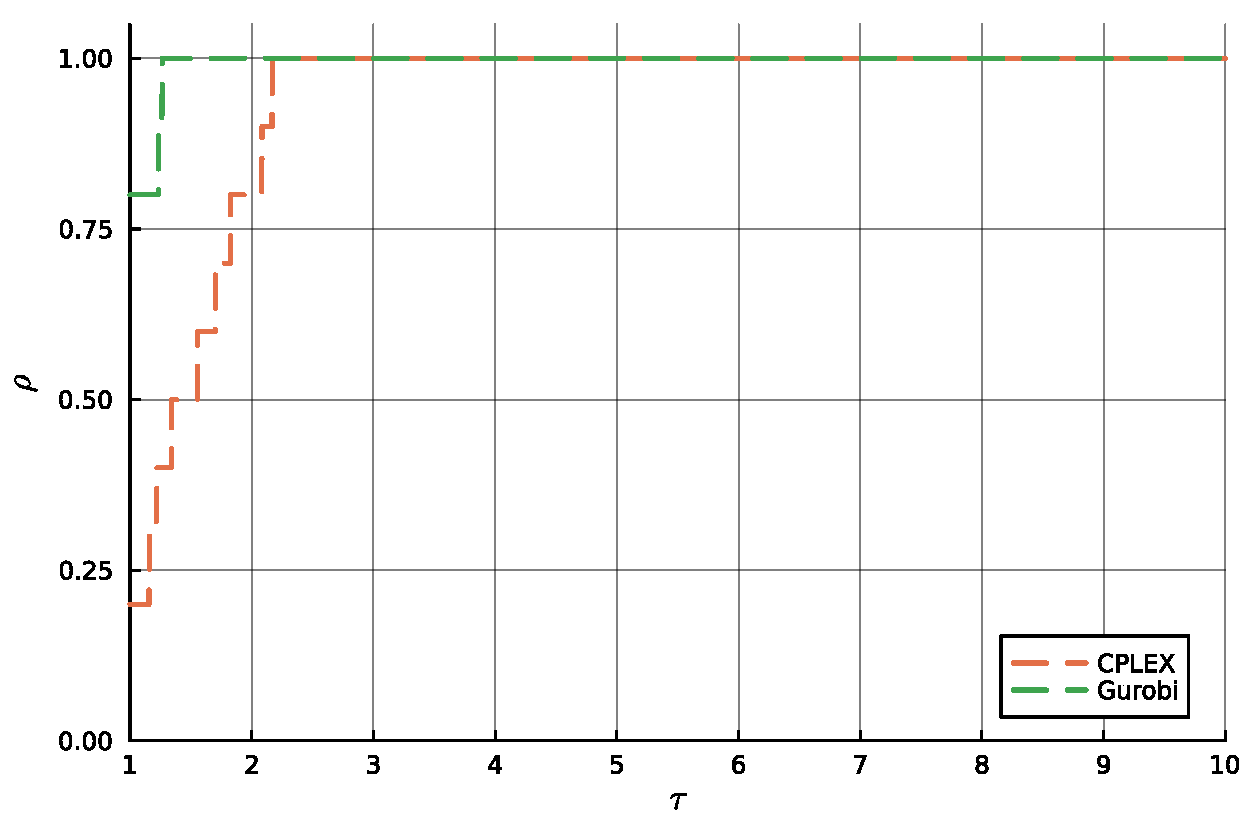
\includegraphics[scale=0.6]{imagens/pgraph50.pdf}
\end{figure}

% \subsection{Problemas de roteamento de veículos}\label{sec:problemas de roteamento de veículos}

% Problemas de roteamento de veículos (PRVs) são extensões do PCV onde mais do que um veículo passa a ser considerado \cite{OR-Tools-VRP}. Geralmente, estes problemas também acrescentam restrições para representar situações mais realistas no roteamento. De particular interesse aqui são o problema de roteamento de veículos capacitado (PRVC) e o problema de roteamento de veículos com janela de tempo (PRVJT).

% O PRVC considera uma frota de veículos com capacidade máxima. Os veículos devem deixar o depósito e realizar entregas de modo que seja necessário apenas um veículo para abastecer cada ponto; ou seja, a capacidade dos veículos deve ser respeitada. O PRVJT, por sua vez, é uma extensão do PRVC, considerando que cada ponto deve ser atendido dentro de determinado intervalo de tempo.

% Existem várias maneiras de formular o PRVJT. Nesta seção, utilizaremos a mostrada por Vieira \cite{VIEIRA:13}, com uma notação um pouco diferente. Considere $\mcal{V}$ o conjunto de vértices do problema, $K$ o conjunto de veículos utilizados, $C$ a capacidade máxima dos veículos, $m_i$ as demandas respectivas dos vértices $v_i$ e $v(S)$ o número de veículos necessários para atender completamente a demanda de um conjunto de vértices $S$.

% Com as variáveis descritas até aqui, temos o suficiente para representar um PRVC. Para representar um PRVJT, entram em jogo as variáveis $b_i$, que indicam o momento de chegada de um veículo a cada vértice $v_i$; $s_i$, que indicam o tempo necessário para atender cada vértice $v_i$; e $t_{ij}$, que indicam o tempo de deslocamento dos vértice $v_i$ para os vértices $v_j$. Por fim, as variáveis $b_i$ e $l_i$ indicam, respectivamente, o começo e o fim do intervalo de tempo em que os vértices estão disponíveis para atendimento.

% Denotando $\mcal{V}\fast = \mcal{V}\backslash\{0\}$, temos o seguinte modelo de PRVJT:

% \begin{subequations}
% \begin{align}
%     \min&\sum_{\substack{i\in \mcal{V} \\ j\in \mcal{V} \\ k\in K}}\vcc{ij}\x{ijk} \label[expression]{eq:prvjt1}\\
%     \text{s.a }&\sum_{\substack{k \in \mcal{V} \\ j \in \mcal{V}\fast}} \x{0jk} \leq |K|,& \label[constraint]{eq:prvjt2}\\
%     &\sum_{j\in \mcal{V}\fast}\x{0jk} = \sum_{j\in \mcal{V}\fast}\x{j0k} \leq 1,&\forall k \in K,& \label[constraint]{eq:prvjt3}\\
%     &\sum_{\substack{k\in K \\ j\in \mcal{V}}}\x{ijk} = 1,&\forall i \in \mcal{V}\fast,& \label[constraint]{eq:prvjt4}\\
%     &\sum_{j\in \mcal{V}}\x{ijk} = \sum_{j \in \mcal{V}}\x{jik},&\forall k \in K,\ i \in \mcal{V}\fast,& \label[constraint]{eq:prvjt5}\\
%     &\sum_{\substack{i\in S \\ j\in S \\ k \in K}}\x{ijk} \leq |S| - v(S),&\forall S \subseteq \mcal{V}\fast,\ |S| \geq 2,& \label[constraint]{eq:prvjt6}\\
%     &\sum_{\substack{i\in \mcal{V}\fast\\j\in \mcal{V} \\ j \neq i}}m_i\x{ijk} \leq C,&\forall k \in K,& \label[constraint]{eq:prvjt7}\\
%     &\sum_{\substack{k \in K \\ i \in \mcal{V} \\ i \neq j}}\x{ijk}(b_i + s_i + t_{ij}) \leq b_j,&\forall j \in \mcal{V}\fast,& \label[constraint]{eq:prvjt8}\\
%     &e_i \leq b_i \leq l_i,&\forall i \in \mcal{V},& \label[constraint]{eq:prvjt9}\\
%     &\x{ijk} \in \{0,1\},&\forall i, j \in \mcal{V},\ k \in K \label[constraint]{eq:prvjt10}.
% \end{align}
% \end{subequations}

% A \cref{eq:prvjt1} generaliza o problema de minimização para vários veículos, enquanto a \cref{eq:prvjt2} garante que o número de veículos utilizados não exceda o total da frota. As \cref{eq:prvjt3,eq:prvjt4,eq:prvjt5} asseguram que todas as rotas terão início e fim no depósito; que de cada ponto (salvo o depósito) ocorre a partida de apenas um veículo; e que um veículo que entre em um ponto deve também sair deste ponto.

% A \cref{eq:prvjt6} é uma versão ampliada da restrição anti-subciclo introduzida na modelagem do PCV, na \cref{sec:pcv}. Note que o número máximo aceitável de deslocamentos dentro de um subconjunto de pontos do problema foi alterado de ${|S| - 1}$ para ${|S| - v(S)}$. Para entender esta alteração, imagine que ${v(S) \geq 1}$ veículos precisem atender um subconjunto de $|S|$ pontos. Como cada veículo inicia sua trajetória neste conjunto a partir de um dos seus pontos, restam $|S| - v(S)$ pontos pelos quais estes veículos podem passar sem voltar a um ponto que já foi atendido anteriormente. Portanto, ${|S| - v(S)}$ é o número máximo de deslocamentos que pode acontecer sem que ocorra formação de subciclos no subconjunto de pontos $S$. Por fim, note que a modelagem de Vieira inclui ainda a condição $S \subseteq \mcal{V}\fast$ nesta restrição, pois a \cref{eq:prvjt3} força todos os veículos que partirem do depósito a retornar para ele, o que torna sua inclusão redundante.

% A \cref{eq:prvjt7} garante que nenhum veículo tenha que entregar mais carga do que consegue comportar. Segundo Vieira, esta restrição é redundante, pois a \cref{eq:prvjt6} implicitamente garante os mesmos resultados.

% A \cref{eq:prvjt8} assegura que os veículos cheguem em horários adequados aos pontos que devem atender. Assim, é necessário que a soma do tempo de chegada ao ponto $i$, do tempo de atendimento ao ponto $i$ e do tempo de deslocamento do ponto $i$ ao $j$ resulte em um tempo igual ou anterior ao momento em que se espera começar a atender o ponto $j$. Este tempo é delimitado pela \cref{eq:prvjt9}, devendo estar dentro do intervalo de disponibilidade do ponto ao qual se chega. Note que a \cref{eq:prvjt8} força os veículos a se deslocarem por entre pontos diferentes, o que impede a formação de subciclos de um único ponto. É por esta razão que a \cref{eq:prvjt6} impõe a condição $\ |S| \geq 2$.

% Existem várias outras considerações a fazer, a depender do caso. Por exemplo, Kallehauge \emph{et al.} \cite{KALLEHAUGE:05} apresentam a possibilidade de se modelar o problema considerando que diferentes veículos podem levar diferentes tempos para atender a certos pontos. Isso introduz não-linearidades ao modelo, deixando sua resolução mais complexa. No fim das contas, é necessário avaliar quão realista e precisa a modelagem de um problema tem que ser para optar por um modelo ou outro.
\section{Problemas de roteamento de veículos com janelas de tempo}\label{sec:PRVJT}
O objetivo desta seção é introduzir problemas de roteamento de veículos (PRVs), que são generalizações do PCV para frotas \cite{DANTZIG:59}. Existem vários tipos de PRVs, cada qual com suas próprias famílias de restrições \cite{TORO:16,VIEIRA:13}. Uma consequência desta variedade é que a complexidade computacional dos PRVs é maior do que a do PCV, fato que se reflete no empenho muito maior da comunidade científica em encontrar soluções exatas para o PCV do que para PRVs \cite{LAPORTE:87}.

O PRV com janelas de tempo (PRVJT) considera que cada ponto tem uma janela de tempo específica para ser atendido por um veículo. Como o PRVJT não considera o nível de combustível dos veículos, ele é mais apropriado para criar modelos básicos para ônibus a combustão, cujo combustível dura mais e pode ser reabastecido rapidamente. As janelas de tempo de cada região a ser atendida podem ser definidas conforme o planejamento urbano da cidade.

\subsection{Modelo genérico}\label{sec:PRVJT genérico}
\textcite{VIEIRA:13} apresenta o seguinte modelo de PRVJT, que é uma extensão de um problema capacitado (PRVC), em que os veículos têm uma capacidade máxima de carga e cada ponto tem sua própria demanda. Uma implementação básica deste modelo pode ser encontrada no \cref{sec:implementação PRVJT genérico}.

\begin{align}
    \min&\sum_{\substack{i,j\in \mcal{V}\\ k\in K}}c_{ij}x_{ijk} \label[expression]{eq:prvjt1}\\
    \text{s.a }&\sum_{\substack{k \in K \\ j \in \mcal{V}\fast}} x_{0jk} \leq |K|,& \label[constraint]{eq:prvjt2}\\
    &\sum_{j\in \mcal{V}\fast}x_{0jk} = \sum_{j\in \mcal{V}\fast}x_{j0k} \leq 1,&\forall k \in K,& \label[constraints]{eq:prvjt3}\\
    &\sum_{\substack{k\in K \\ j\in \mcal{V}}}x_{ijk} = 1,&\forall i \in \mcal{V}\fast,& \label[constraints]{eq:prvjt4}\\
    &\sum_{j\in \mcal{V}}x_{ijk} - \sum_{j \in \mcal{V}}x_{jik} = 0,&\forall k \in K,\ i \in \mcal{V}\fast,& \label[constraints]{eq:prvjt5}\\
    &\sum_{\substack{i,j\in S \\ k \in K}}x_{ijk} \leq |S| - v(S),&\forall S \subseteq \mcal{V}\fast,\ |S| \geq 2,& \label[constraints]{eq:prvjt6}\\
    &\sum_{\substack{k \in K \\ i \in \mcal{V} \\ i \neq j}}x_{ijk}(b_i + s_i + t_{ij}) \leq b_j,&\forall j \in \mcal{V}\fast,& \label[constraints]{eq:prvjt7}\\
    &e_i \leq b_i \leq l_i,&\forall i \in \mcal{V},& \label[constraints]{eq:prvjt8}\\
    &x_{ijk} \in \{0,1\},&\forall i, j \in \mcal{V},\ k \in K \label[constraints]{eq:prvjt9}.
\end{align}

Esta formulação considera o problema como um grafo $G = (\mcal{V}, \mcal{A})$. O depósito é o vértice $0$, e $\mcal{V}\fast = \mcal{V} \backslash \{0\}$. Considera-se uma frota $K$ de veículos homogêneos de capacidade $Q$, e para cada ponto existe uma variável $m_i$ indicando sua demanda. As variáveis $e_i$ e $l_i$ indicam o início e o fim do intervalo de atendimento a cada ponto, inclusive do depósito. A variável $b_i$ indica o horário em que um veículo chega ao ponto $i$; $s_i$ indica o tempo de atendimento ao ponto $i$; $t_{ij}$ indica o tempo de deslocamento necessário entre $i$ e $j$.

A \cref{eq:prvjt1} define o problema de minimização de distâncias. Usam-se $|K|$ matrizes de adjacência, uma para cada veículo. A \cref{eq:prvjt2} garante que não saiam do depósito mais veículos do que a frota comporta. Também é possível garantir que todos os veículos saiam do depósito, transformando a inequação em equação, ou considerando o depósito como sendo dois vértices distintos, $0$ e $n + 1$. Neste caso, os veículos que não forem utilizados farão ciclo entre $0$ e $n + 1$ \cite{SHERBENY:10}. As \cref{eq:prvjt3} asseguram que todos os veículos saiam e retornem ao depósito. As \cref{eq:prvjt4} faz com que apenas um veículo atenda cada ponto. As \cref{eq:prvjt5} garantem que os veículos saiam de todos os pontos nos quais entrarem.

As \cref{eq:prvjt6} impedem que sejam formados ciclos que violem as capacidades dos veículos. A função $v(S)$ retorna o número mínimo de veículos necessários para atender o conjunto de pontos. É possível defini-la como

\begin{equation}
    v(S) = \left\lceil\sum_{i \in S}\frac{m_i}{Q}\right\rceil.
\end{equation}

Supondo um conjunto de $n$ pontos, se $m$ veículos forem necessários para atendê-los, então restam a estes veículos $n - m$ pontos para os quais se deslocar. Quaisquer deslocamentos a mais entre os pontos de $S$ denunciam violações às restrições de capacidade dos veículos.

As \cref{eq:prvjt7} asseguram que o veículo que vai de $i$ a $j$ finalizará o seu atendimento a $i$ a tempo de chegar a $j$ no horário de atendimento. As \cref{eq:prvjt8} garantem que todos os veículos cheguem aos pontos de entrega dentro da janela de tempo definida para cada ponto. Por fim, as \cref{eq:prvjt9} garantem que as variáveis de decisão sejam todas inteiras.

As \cref{eq:prvjt7} têm comportamento não-linear, pois tanto $x_{ijk}$ quanto $b_i$ são variáveis de decisão. \textcite{KALLEHAUGE:05,CORDEAU:05} propõem linearizar esta expressão trocando-a por outra da forma

\begin{equation}
    b_i + s_i + t_{ij} - M_{ij}(1 - x_{ijk}) \leq b_j,\ \forall i,j \in \mcal{V}, \forall k \in K,\label[constraints]{eq:linearização}
\end{equation}
onde $M_{ij}$ é uma constante cujo valor precisa ser, no mínimo, $\max\{l_i + t_{ij} - e_j\}$, $(i,j) \in \mcal{A}$.

É possível utilizar as restrições de capacidade para definir um número máximo de pontos que cada ônibus possa atender. Se capacidades não forem uma preocupação, é possível escolher $Q \to \infty$.

\subsection{Modelo escolar com rotas pré-determinadas}

Problemas em uma mesma categoria podem ter formulações radicalmente diferentes, a depender das considerações matemáticas tecidas. \textcite{FÜGENSCHUH:04}, por exemplo, propõem um modelo de PRVJT que permite a roteirização de ônibus escolares que também podem ser usufruídos pela população geral. Este modelo considera $\mcal{S}$ o conjunto de escolas a serem atendidas. Para toda escola $s \in \mcal{S}$, é definida uma janela de tempo de atendimento $[\underline{\tau}_s,\overline{\tau}_s]$, com $\underline{\tau}_s,\overline{\tau}_s\in \mathbb{Z_+}$.

Esta formulação define como \emph{viagens}\footnote{\emph{"Trips".}} as sequências de pontos pelas quais cada ônibus deve passar até chegar a cada escola. Trabalha-se com um conjunto já definido de viagens, $\mcal{V}$, com cada viagem individual sendo representada por $t \in \mcal{V}$, e cada aresta que conecta os pontos das viagens estando contida em $\mcal{A}$. As constantes $\underline{\alpha}_t$ e $\overline{\alpha}_t$, com $\underline{\alpha}_t \leq \overline{\alpha}_t$ e $\underline{\alpha}_t, \overline{\alpha}_t\in \mathbb{Z}_+$, definem o intervalo aceitável de valores para $\alpha_t$, que indica quando a viagem $t$ é iniciada. O tempo entre o início e o fim de uma viagem é $\delta_t^{\text{trip}} \in \mathbb{Z_+}$.

$\mcal{P}$ é definido como o conjunto das tuplas $(s,t)$ que associam uma viagem $t$ a uma escola $s$. O tempo entre o início e o fim de uma viagem até uma escola é $\delta_t^{\text{school}}\in \mathbb{Z_+}$. O intervalo $[\underline{\omega}_{st}^{\text{school}},\overline{\omega}_{st}^{\text{school}}]$, com $\underline{\omega}_{st}^{\text{school}},\overline{\omega}_{st}^{\text{school}} \in \mathbb{Z_+}$, define quanto tempo os alunos podem esperar pelo ônibus.

É possível que um aluno precise passar por mais do que uma viagem para chegar à sua escola. Neste caso, considera-se o conjunto $\mcal{C}$ de tuplas $(t_1,t_2)$, que representam uma \emph{troca}\footnote{\emph{"Change".}} da viagem $t_1$ para a viagem $t_2$. A viagem $t_1$ é chamada de \emph{feeder}, e $t_2$ é chamada de \emph{collector}. O tempo decorrido entre o começo de uma viagem \emph{feeder} e a chegada até o ponto de troca é $\delta_{t_1t_2}^{\text{feeder}} \in \mathbb{Z_+}$. Já o tempo que o ônibus que coleta os alunos deixados leva para chegar a este ponto é $\delta_{t_1t_2}^{\text{collector}} \in \mathbb{Z_+}$. O intervalo de tempo aceitável de espera no ponto que conecta as duas viagens é $[\underline{\omega}_{t_1t_2}^{\text{change}}, \overline{\omega}_{t_1t_2}^{\text{change}}]$, com $\underline{\omega}_{t_1t_2}^{\text{change}}, \overline{\omega}_{t_1t_2}^{\text{change}} \in \mathbb{Z}_+.$

Ônibus que tiverem terminado suas viagens retornam ao depósito. A conexão entre viagens servidas por um mesmo ônibus é chamada de \emph{bloco}. O deslocamento entre o último ponto de uma viagem $t_1$ e o primeiro ponto de uma viagem $t_2$ são chamados de \emph{shifts}. O tempo necessário para completar um \emph{shift} é $\delta_{t_1t_2}^{\text{shift}} \in \mathbb{Z}_+$.

A cada viagem são associadas variáveis $v_t$ e $w_t$, sendo $v_t = 1$ se $t$ for a primeira viagem em um bloco, ou $0$ do contrário. A variável $w_t$ é igual a $1$ se $t$ for a última viagem do bloco, ou $0$ do contrário. Também consideram-se variáveis $x_{t_1t_2} \in \{0,1\}$, com $x_{t_1t_2} = 1$ apenas se um ônibus servir $t_2$ após servir $t_1$.

O modelo proposto pelos autores é:

\begin{align}
    \min&\sum_{t \in \mcal{V}}C_tv_t + \sum_{(t_1,t_2) \in \mcal{A}}\delta_{t_1t_2}^{\text{shift}}x_{t_1t_2},\label[expression]{eq:fugenschuh1}\\
    \text{s.a }&\sum_{(t_1,t_2) \in \mcal{A}}x_{t_1t_2} + v_{t_2} = 1,&\forall t_2 \in \mcal{V},\label[constraints]{eq:fugenschuh2}\\
    &\sum_{(t_1,t_2) \in \mcal{A}}x_{t_1t_2} + w_{t_1} = 1,&\forall t_1 \in \mcal{V},\label[constraints]{eq:fugenschuh3}\\
    &\alpha_{t_1} + \delta_{t_1}^{\text{trip}} + \delta_{t_1t_2}^{\text{shift}} - M (1-x_{t_1t_2}) \leq \alpha_{t_2},&\forall(t_1,t_2) \in \mcal{A},\label[constraints]{eq:fugenschuh4}\\
    &\alpha_{t_1} + \delta_{t_1t_2}^{\text{feeder}} + \underline{\omega}_{t_1t_2} \leq \alpha_{t_2} + \delta_{t_1t_2}^{\text{collector}},&\forall(t_1,t_2)\in\mcal{C},\label[constraints]{eq:fugenschuh5}\\
    &\alpha_{t_1} + \delta_{t_1t_2}^{\text{feeder}} + \overline{\omega}_{t_1t_2} \geq \alpha_{t_2} + \delta_{t_1t_2}^{\text{collector}},&\forall(t_1,t_2)\in\mcal{C},\label[constraints]{eq:fugenschuh6}\\
    &\alpha_t + \delta_{st}^{\text{school}} + \underline{\omega}_{st}^{\text{school}} \leq \underline{\tau}_s + 5\tau_s,&\forall(s,t) \in \mcal{P},\label[constraints]{eq:fugenschuh7}\\
    &\alpha_t + \delta_{st}^{\text{school}} + \overline{\omega}_{st}^{\text{school}} \geq \underline{\tau}_s + 5\tau_s,&\forall(s,t) \in \mcal{P}.\label[constraints]{eq:fugenschuh8}
\end{align}

A \cref{eq:fugenschuh1} indica que este é um problema de minimização biobjetivo. Deseja-se minimizar as distâncias percorridas e o tempo de \emph{shift} dos ônibus que servirem blocos. As \cref{eq:fugenschuh2} asseguram que cada viagem será ou a primeira realizada por um ônibus, ou estará conectada a uma viagem anterior. Por outro lado, as \cref{eq:fugenschuh3} garantem que cada viagem seja a última, ou que seja antecessora de outra.

As \cref{eq:fugenschuh4} garantem que todos os ônibus que conectam viagens $t_1$ e $t_2$ completem $t_1$ a tempo de começarem $t_2$. As \cref{eq:fugenschuh5,eq:fugenschuh6} forçam os ônibus de viagens do tipo \emph{collector} a chegarem aos pontos de coleta dentro do intervalo aceitável de espera dos alunos. As \cref{eq:fugenschuh7,eq:fugenschuh8} definem os tempos de início das aulas para cada escola\footnote{As \cref{eq:fugenschuh5,eq:fugenschuh6,eq:fugenschuh7,eq:fugenschuh8} criam dependências entre as janelas de tempo, razão pela qual os autores classificam o modelo completo como um PRV de \emph{coupled time windows} (CTW).}. Neste caso, os autores consideraram que os tempos aceitáveis sejam separados por intervalos de 5 minutos, com

\begin{equation}
    \tau_s = \frac{\overline{\tau_s} - \underline{\tau_s}}{5}.
\end{equation}

Posteriormente, \textcite{FÜGENSCHUH:09} apresentou uma versão expandida deste modelo, com testes de caso para escolas alemãs. Constatou-se que seria possível diminuir de 10 a 25\% a frota de ônibus em operação nos locais selecionados.

\subsection{Modelo de frota mista}
As dificuldades associadas à aquisição de ônibus elétricos destacadas na \cref{sec:dificuldades de implementação} tornam uma modelagem mista interessante. Nesta seção, é apresentado um modelo de \emph{Electric Fleet Size and Mix Vehicle Routing Problem with Time Windows and recharging stations} (\emph{E-FSMFTW})\footnote{Uma possível tradução para o português seria "PRVJT com tamanho de frota elétrica, veículos mistos e estações de recarga".} proposto por \textcite{HIERMANN:16}.

A notação dos autores considera que $C$ é o conjunto de pontos a serem atendidos e $F$ é o conjunto das estações de recarga. Existe um único depósito e um conjunto $V$ de tipos de veículos. Considera-se o conjunto $N = C \cup F'$, onde $F'$ é um conjunto de cópias dos pontos de $F$. Este conjunto é criado para que vários ônibus elétricos possam acessar uma mesma estação de recarga. O depósito é representado pelo vértice de partida $u_0$ e o vértice de chegada $u_{n+1}$. Tem-se ainda $N_0 = N \cup \{u_0\}$, $N_{n+1} = N \cup \{u_{n+1}\}$ e $N_{0,n+1} = N_0 \cup N_{n+1}$. A mesma notação se aplica a $C$ e $F'$. Além disso, existem variáveis $x_{ij}^k \in \{0,1\}$, com $x_{ij}^k = 1$ apenas se um veículo do tipo $k \in V$ se desloca do ponto $i$ ao ponto $j$.

As variáveis $Q^k$ definem a capacidade máxima de veículos do tipo $k$. A cada ponto $i$ estão associadas uma variável de demanda, $p_i$, e uma variável com a carga atual do veículo de tipo $k$ que o atende, $q_i^k$. Da mesma forma, $Y^k$ representa a capacidade energética máxima dos veículos do tipo $k$, com $y_i^k$ representando a energia atual do veículo de tipo $k$ que atende o ponto $i$. O consumo energético por unidade de distância percorrida por veículos do tipo $k$ é $r^k$, e o tempo de recarga por unidade de energia é $g^k$.

Para definir janelas de tempo, os autores usam as variáveis $e_i$, $l_i$, $s_i$, $t_{ij}$, com os mesmos significados atribuídos por \textcite{VIEIRA:13} na \cref{sec:PRVJT genérico}, e $\tau_i$, que representa o momento em que o veículo começa a atender o ponto $i$. Consideram-se ainda a variável $d_{ij}$, que expressa a distância do ponto $i$ ao ponto $j$, o custo de aquisição de veículos do tipo $k$, representado por $f^k$, e o custo de deslocar um veículo do tipo $k$ do ponto $i$ ao ponto $k$, denotado por $c_{ij}^k$.

Com esta notação, os autores modelam o problema da seguinte maneira:

\begin{footnotesize}
\begin{align}
    \min& \sum_{\substack{k \in V\\j \in N}}f^kx_{0j}^k + \sum_{\substack{k \in V\\i \in N_0\\j \in N_{n+1}\\i \neq j}}c_{ij}^kx_{ij}^k\label[expression]{eq:hiermann1}\\
    \text{s.a }& \sum_{\substack{k \in V\\j \in N_{n+1}\\i \neq j}}x_{ij}^k = 1, & \forall i \in C, \label[constraints]{eq:hiermann2}\\
    &\sum_{\substack{k \in V\\j \in N_{n+1}\\i \neq j}}x_{ij}^k \leq 1, & \forall i \in F', \label[constraints]{eq:hiermann3}\\
    &\sum_{\substack{i \in N_{n+1}\\ i \neq j}}x_{ji}^k - \sum_{\substack{i \in N_0\\ i \neq j}}x_{ij}^k = 0, & \forall j \in N, k \in V, \label[constraints]{eq:hiermann4}\\
    &e_j \leq \tau_j \leq l_j, & \forall j \in N_{0,n+1}, \label[constraints]{eq:hiermann5}\\
    &\tau_i + (t_{ij} + s_i)x_{ij}^k - l_0(1 - x_{ij}^k) \leq \tau_j, & \forall k \in V, i \in C_0, j \in N_{n+1}, i \neq j, \label[constraints]{eq:hiermann6}\\
    &\tau_i + t_{ij}x_{ij}^k + g^k(Y^k - y_i^k) - (l_0 + g^kY^k)(1 - x_{ij}^k) \leq \tau_j, & \forall k \in V, i \in F', j \in N_{n+1}, i \neq j, \label[constraints]{eq:hiermann7}\\
    &q_j^k \leq q_i^k - p_ix_{ij}^k + Q^k(1 - x_{ij}^k), & \forall k \in V, i \in N_0, j \in N_{n+1}, i \neq j, \label[constraints]{eq:hiermann8}\\
    &0 \leq q_j^k \leq Q^k, & \forall k \in V, j \in N_{0, n+1}, \label[constraints]{eq:hiermann9}\\
    &0 \leq y_j^k \leq y_i^k - (r^kd_{ij})x_{ij}^k + Y^k(1 - x_{ij}^k), & \forall k \in V, i \in C, j \in N_{n+1}, i \neq j, \label[constraints]{eq:hiermann10}\\
    &0 \leq y_j^k \leq Y^k - (r^kd_{ij})x_{ij}^k, & \forall k \in V, i \in F_0', j \in N_{n+1}, i \neq j, \label[constraints]{eq:hiermann11}\\
    &y_0^k = Y^k, & \forall k \in V, \label[constraints]{eq:hiermann12}\\
    &x_{ij}^k \in \{0,1\}, & \forall i \in N_0, j \in N_{n+1}, i \neq j, k \in V. \label[constraints]{eq:hiermann13}
\end{align}
\end{footnotesize}

A \cref{eq:hiermann1} estabelece um problema biobjetivo. O primeiro objetivo é minimizar os gastos de aquisição dos veículos que sairão do depósito. O segundo objetivo é minimizar o custo total associado aos deslocamentos de cada tipo de veículo. As \cref{eq:hiermann2} forçam que apenas um veículo passe por cada ponto do problema. As \cref{eq:hiermann3} permitem que os veículos elétricos façam (ou não) recarga nas estações. As \cref{eq:hiermann4} asseguram que todos os veículos entrem e saiam de cada vértice, salvo o caso especial do depósito, que é representado por dois vértices.

As \cref{eq:hiermann5,eq:hiermann6} são análogas às \cref{eq:prvjt7,eq:linearização}, com $l_0$ correspondendo a $M$. As \cref{eq:hiermann7} garantem que os veículos não gastem mais tempo recarregando suas baterias ao máximo do que o necessário para começar a atender o próximo ponto. A constante $l_0 \to \infty$ tenta garantir que esta família de restrições não afete veículos que não se deslocarem de uma estação de recarga $i$ a um ponto de atendimento $j$. Como as unidades de energia usadas podem variar, é possível que $l_0 < g^k(Y^k - y_i^k)$. Para evitar que isso quebre o modelo, soma-se $g^kY^k$ a $l_0$, pois $l_0 + g^kY^k > g^k(Y^k - y_i^k)$.

As \cref{eq:hiermann8} garantem que as cargas dos veículos sejam atualizadas ao longo dos seus trajetos, enquanto as \cref{eq:hiermann9} asseguram que os veículos não façam viagens cuja demanda total exceda suas capacidades. As \cref{eq:hiermann10,eq:hiermann11} funcionam analogamente, atualizando as energias dos veículos e garantindo que não seja utilizada mais energia do que a bateria do respectivo veículo permite. Por fim, as \cref{eq:hiermann12} asseguram que todos os veículos comecem a operar com o máximo de energia, e as \cref{eq:hiermann13} estabelecem que as variáveis de decisão dos deslocamentos são binárias.

Este modelo pode ser expandido para considerar recargas parciais. Isso é preferível, pois o ideal para baterias de lítio é que sua carga seja mantida entre 65 e 75\% do valor máximo. Além disso, a não-linearidade de recarga das baterias pode ser contabilizada para garantir uso mais preciso das baterias e do tempo. Formulações mais aprofundadas, como as de \textcite{CATALDO:22,ZHANG:21,HELLMARK:22,ZUO:19}, levam em conta tais fatores.

\subsection{Comparação de modelos}
Os três modelos apresentados nesta seção (genérico \cite{VIEIRA:13}, escolar \cite{FÜGENSCHUH:04}, frota mista \cite{HIERMANN:16}) demonstram a grande variabilidade das formulações de PRVJTs, advindas das considerações feitas em diferentes contextos. A seguir, estão listadas algumas diferenças e similaridades notáveis.

\subsubsection*{Função objetivo}
O modelo \cite{VIEIRA:13} possui apenas um objetivo de minimização, enquanto \cite{FÜGENSCHUH:04,HIERMANN:16} possuem dois. Parece ser uma tendência dos modelos mais complexos serem pelo menos biobjetivos, dada a profundidade das suas considerações acerca dos veículos utilizados. Outros exemplos desta tendência incluem \cite{KESKIN:18,CATALDO:22,FROGER:17,ZUO:19,ZHANG:21}.

\subsubsection*{Variáveis de decisão}
O modelo \cite{FÜGENSCHUH:04} se distingue dos demais por considerar rotas já planejadas. Assim, este modelo não se utiliza da ideia de matrizes de adjacência. O modelo \cite{VIEIRA:13} considera várias matrizes de adjacência, uma para cada veículo da frota, ao passo que \cite{HIERMANN:16} considera que veículos distintos de um mesmo tipo compartilham da mesma matriz de adjacência, de modo similar à modelagem em \cite{ACHUTHAN:96}. Tendo em vista as considerações computacionais realizadas na \cref{sec:considerações computacionais}, esta última abordagem é preferível, pois economiza variáveis inteiras.

\subsubsection*{Janelas de tempo}
Em \cite{VIEIRA:13,HIERMANN:16}, as janelas de tempo são pré-definidas. Em \cite{FÜGENSCHUH:04}, um dos desafios é definir quais são os horários ótimos para as janelas de tempo. Isso se deve ao fato de \cite{FÜGENSCHUH:04} abordar um problema de planejamento urbano, ao passo que \cite{VIEIRA:13,HIERMANN:16} são modelos pensados para entregas, cujos horários são controlados por fatores externos.

\subsubsection*{Garantia da factibilidade}
Em \cite{VIEIRA:13}, a factibilidade do modelo é garantida por restrições sobre todos os subconjuntos de pontos do problema, de maneira similar à formulação DFJ do PCV. Em \cite{FÜGENSCHUH:04}, ela é garantida pelo ajuste mútuo das janelas de tempo. Já \cite{HIERMANN:16} assegura a factibilidade do modelo por meio de janelas de tempo, além de produzir cópias das estações de recarga do modelo para garantir que vários veículos possam passar pelo mesmo vértice. Como \cite{FÜGENSCHUH:04} trabalha com rotas já conhecidas, o modelo evita este aumento de complexidade computacional.
\include{conclusão.tex}

%\nocite{*}
\printbibliography

\appendix
\section{O método simplex}\label{sec:metodo_simplex}
\subsection{Teoremas fundamentais para o método simplex}\label{sec:simplex pontos extremos}

\begin{mydef}[Reta]\label{def:reta}
Um poliedro $\vb P \subset \mathbb{R}^n$ contém uma \emph{reta} se existem um vetor $x \in \vb P$ e um vetor não-nulo $ d \in \mathbb{R}^n$ tais que $x + \lambda d \in \vb P$ para todo escalar $\lambda$.
\end{mydef}

\begin{theorem}\label{teo:retas}
    Suponha que o poliedro ${\vb P = \{x \in \mathbb{R}^n \mid a_i^\intercal x \leq b_i, i = 1,\ldots,m\}}$ é não-vazio. Então segue-se que:
    \begin{enumerate}[(a)]
    \item $\vb P$ tem pelo menos um ponto extremo.
    \item $\vb P$ não contém reta.
    \item Existem $n$ vetores da família $a_1,\ldots,a_m$ que são linearmente independentes.
    \end{enumerate}
\end{theorem}

\begin{proof}
    $(b) \Rightarrow (a)$

    Sejam $x \in \vb P$ e $ \vb I = \{i\mid a_i^\intercal x = b_i\}$. Se $n$ vetores $a_i, i \in  \vb I$, forem linearmente independentes, então $x$ é, por definição, uma solução básica factível e, portanto, existe ponto extremo em $\vb P$. Se este não for o caso, todos os vetores $ a_i, i \in  \vb I$, pertencem a um subespaço próprio de $\mathbb{R}^n$ e, destarte, existe um vetor $d \neq \vb 0$ tal que $a_i^\intercal d = 0$ para todo $i \in  \vb I$. Seja $y = x + \lambda  d$ uma reta, com $\lambda$ sendo um escalar arbitrário. Para $i \in  \vb I$, temos

    $$a_i^\intercal y = a_i^\intercal x + \lambda a_i^\intercal d = a_i^\intercal x = b_i.$$

    Logo, as restrições ativas em $ x$ permanecem ativas ao longo de toda a reta $ y$. Contudo, como estamos assumindo $(b)$ como hipótese, segue-se que, variando $\lambda$, estaremos eventualmente violando uma restrição. Na iminência de uma tal violação, uma nova restrição deve ficar ativa. Logo, existem $\lambda^*$ e $j \notin  \vb I$ tais que $a_j^\intercal (x + \lambda^*d) = b_j$.

    Vamos provar que $ a_j$ não é combinação linear dos vetores $ a_i, i \in  \vb I$. Temos que $a_j^\intercal x \neq b_j$ (pois $j \notin  \vb I$) e $a_j^\intercal (x + \lambda^*d) = b_j$ (pela definição de $\lambda^*$). Assim, $a_j^\intercal d \neq 0$. Por outro lado, $a_i^\intercal d = 0$ para todo $i \in  \vb I$ (pela definição de $ d$) e, portanto, $ d$ é ortogonal a qualquer combinação linear dos vetores $ a_i, i \in  \vb I$. Como $ d$ não é ortogonal a $ a_j$, concluímos que $ a_j$ não é combinação linear dos vetores $ a_i, i \in  \vb I$.

    Logo, no deslocamento do ponto $ x$ para $ x + \lambda^* d$, o número de restrições linearmente independentes aumenta em pelo menos um. Repetindo este argumento tantas vezes quanto for necessário, eventualmente chegamos a um ponto em que $n$ restrições são ativas. Por definição, este ponto é solução básica e, como não violamos nenhuma restrição, é solução básica factível e, portanto, um ponto extremo.

    $(a) \Rightarrow (c)$

    Se $x \in \vb P$ é ponto extremo, $ x$ também é solução básica factível, e existem $n$ restrições ativas em $ x$ cujos vetores $ a_i$ são linearmente independentes.

    $(c) \Rightarrow (b)$

    Suponha que $n$ dos vetores $ a_i$ sejam linearmente independentes e, sem perda de generalidade, sejam $a_1,\ldots,a_n$ linearmente independentes. Suponha que $\vb P$ contenha uma reta $ x + \lambda  d$, com $d \neq \vb 0$. Então, temos que $a_i^\intercal (x + \lambda d) \geq b_i$ para todo $i$ e todo $\lambda$. Concluímos que $a_i^\intercal d = 0$ para todo $i$. Como os vetores $ a_i, i = 1,\ldots,n$ são linearmente independentes, segue-se que $d = \vb 0$. Mas isso contradiz o que acabamos de definir para $ d$. Portanto, $\vb P$ não contém retas.
\end{proof}

Finalmente, estamos em condições de introduzir o teorema que justifica a ideia central do método simplex.

\begin{theorem}
    Considere o problema de otimização linear de minimizar $c^\intercal x$ em um poliedro $\vb P$. Suponha que $\vb P$ tenha pelo menos um ponto extremo. Então, ou o custo ótimo é igual a $-\infty$, ou existe um ponto extremo ótimo.
\end{theorem}

\begin{proof}
    Para esta demonstração, considere a seguinte terminologia: um elemento $x \in \vb P$ tem \emph{posto} $k$ se for possível encontrar $k$, e não mais que $k$, restrições linearmente independentes ativas em $x$.

    Suponha que o valor objetivo ótimo é finito. Seja $\vb P = \{x \in \mathbb{R}^n \mid Ax \leq b\}$ e considere $x \in \vb P$ com posto $k < n$. Vamos provar a existência de um $y \in \vb P$ com posto maior que $k$ que também satisfaça $c^\intercal y \leq c^\intercal x$. Seja $ \vb I = \{i\mid a_i^\intercal x = b_i\}$, onde $a_i^\intercal$ é a $i$-ésima linha de $ A$. Como $k < n$, os vetores $ a_i, i \in  \vb I$, pertencem a um subespaço próprio de $\mathbb{R}^n$, e podemos escolher um vetor $ d \in \mathbb{R}^n, d \neq \vb 0$, ortogonal a todo $ a_i, i \in  \vb I$. Ademais, considere que $ d$ é tal que $c^\intercal d \leq 0$.

    Suponha que $c^\intercal d < 0$ e considere a semirreta $y = x + \lambda  d$, onde $\lambda$ é um escalar positivo. Como se segue do \cref{teo:retas}, todos os pontos nesta semirreta satisfazem as relações ${a_i^\intercal y = b_i, i \in  \vb I}$. Se toda a semirreta estivesse contida em $\vb P$, o valor objetivo ótimo seria $-\infty$. Como esta não é nossa hipótese, concluímos que a semirreta sai de $\vb P$ a partir de algum ponto. Na iminência desta saída, temos $\lambda^* > 0$ e $j \notin  \vb I$ tais que $a_j^\intercal (x + \lambda^*d) = b_j$. Então, sendo $y = x + \lambda^* d$, vale que $c^\intercal y < c^\intercal x$. Consequentemente, como mostrado no teorema mencionado, $ a_j$ é linearmente independente em relação a $ a_i, i \in  \vb I$, e o posto de $ y$ é pelo menos $k + 1$.

    Agora suponha que $c^\intercal d = 0$. Seja $y = x + \lambda  d$ uma reta com $\lambda$ escalar arbitrário. Como $\vb P$ não contém retas, a reta precisa sair de $\vb P$ em algum ponto e, na iminência disso, temos outro vetor $ y$ de posto maior que $ x$. Ademais, como $c^\intercal d = 0$, temos $c^\intercal y = c^\intercal x$.

    Em ambos os casos, encontramos $ y$ tal que $c^\intercal y \leq c^\intercal x$ e $\mathrm{posto}( y) > \mathrm{posto}( x)$. Repetindo este processo quantas vezes for necessário, chegamos a um vetor $w$ tal que $\mathrm{posto}(w) = n$ e $c^\intercal w \leq c^\intercal x$.

    Sejam $w^1,\ldots,w^r$ as soluções básicas factíveis em $\vb P$ e seja $w^*$ uma solução básica factível tal que $c^\intercal w^* \leq c^\intercal w^i$ para todo $i$. Já demonstramos que para todo $ x$ existe $i$ tal que ${c^\intercal w^i \leq c^\intercal x}$. Segue-se que ${c^\intercal w^* \leq c^\intercal x}$ para todo $x \in \vb P$, e a solução básica factível $w^*$ é ótima.
\end{proof}

Note que se um poliedro não-vazio não tiver ponto extremo, sua solução ótima é $-\infty$. Pelo contrário, se o poliedro for não-vazio e tiver ponto extremo, sua solução ótima pode ser $-\infty$ ou está localizada em algum dos pontos extremos. Isso nos permite chegar à conclusão necessária para começar a desenvolver o método simplex.

\begin{cor}\label{cor:solução ótima}
Considere o problema de otimização linear de minimizar $c^\intercal x$ em um poliedro não-vazio. Então o custo ótimo é $-\infty$ ou existe solução ótima.
\end{cor}

Deste ponto em diante, chamaremos o caso em que a solução ótima do problema é $-\infty$ de \emph{caso ilimitado}.

\subsection{Considerações iniciais}

Agora que sabemos o exposto pelo \cref{cor:solução ótima}, podemos pensar em uma forma rudimentar de resolver problemas de otimização linear. Uma forma conceitualmente simples é descrita nos passos a seguir.

\begin{enumerate}
    \item Encontrar todas as soluções básicas $x^1,\ldots,x^p$.
    \item Determinar o conjunto $\vb{F} = \{x^i \mid x^i \text{ é factível}\}$.
    \item Encontrar o ponto ótimo $x^* = \min(\vb F)$.
\end{enumerate}

Evidentemente, esta abordagem tem problemas. Primeiramente, esta verificação não considera a possibilidade de a solução ótima ser $-\infty$. Além disso, como evidenciado pela \cref{eq:maxSBF}, existem $\binom{n}{m}$ maneiras de organizar as $n$ variáveis de decisão do problema de maneira que o sistema $\eqsys$ seja satisfeito junto com as restrições de não-negatividade; ou, ainda, existem $p = \binom{n}{m}$ soluções básicas para o problema. Logo, para problemas com número considerável de variáveis e restrições, este método é custoso já no primeiro passo, tornando-se praticamente inviável.

O método simplex implementa uma ideia mais sofisticada do exposto acima. Este método depende de um ponto extremo inicial e, a partir deste ponto, se desloca para um novo ponto extremo a cada iteração. O deslocamento do simplex é condicionado de modo que o método reduza o valor objetivo a cada iteração. Além disso, o método é capaz de determinar se o ponto em que se encontra é ótimo, ou se a solução ótima é $-\infty$, sem ter que compará-lo a todos os outros pontos extremos.

Implementamos o método simplex através de um pacote computacional chamado \texttt{Caique.jl} \cite{Centenaro:23}, que se encontra em um repositório do \emph{GitHub} (\url{https://github.com/phcentenaro7/Caique.jl}). O \texttt{Caique.jl} é um pacote escrito em Julia \cite{JULIA} que pode ser usado para resolver problemas de otimização linear. O código do pacote foi implementado com base nas obras de \textcite{BAZARAA:10,BERTSIMAS:97}, e põe em prática os algoritmos que serão apresentados nesta seção.

\emph{Caique} é o nome em inglês de uma espécie de pássaros conhecida no Brasil como marianinha. Como o método simplex "pula" de um ponto extremo do problema a outro, ele lembra bastante uma das muitas marianinhas saltitantes que podem ser encontradas em vídeos pela internet, servindo de inspiração para o nome do pacote.

\begin{figure}[h!]
    \centering
    \caption{Exemplo de marianinha \cite{BÉKÉSI:09}}
    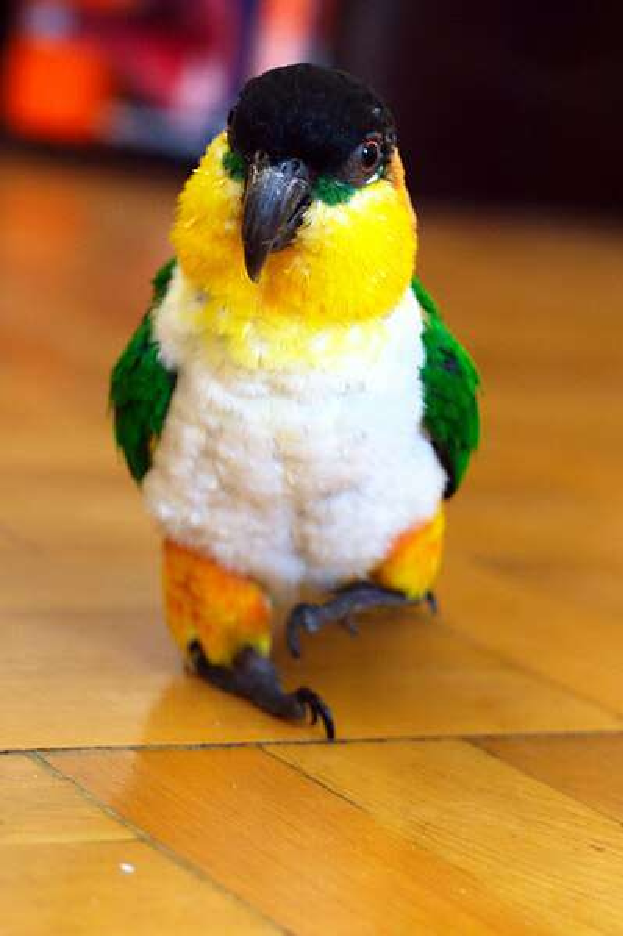
\includegraphics[scale=0.5]{imagens/marianinha.pdf}
\end{figure}


\subsection{Representação de um problema em forma canônica}\label{sec:forma canônica}

Antes de começar o desenvolvimento do simplex, precisamos garantir que o problema de otimização linear esteja na forma \emph{canônica}. Diferentemente da forma padrão, apresentada no \cref{eq:forma padrão}, a forma canônica se apresenta em termos apenas de igualdades, à exceção apenas das restrições de não-negatividade, que continuam as mesmas. O \cref{eq:forma canônica} apresenta a forma canônica.

\begin{align}\label[problem]{eq:forma canônica}
    \min\ &\objval\\
    \textrm{s.a }& \eqsys,\\
    &  x \geq \vb 0.
\end{align}

Neste caso, assim como na forma padrão, $A$ é uma matriz de dimensões $m\times n$, $\vc$ e $ x$ são vetores no $\mathbb{R}^{n}$ e $\vbb$ é um vetor no $\mathbb{R}^m$. 

É possível converter problemas da forma padrão para a forma canônica de modo que continuem os mesmos. Para tal, faremos uso de \emph{variáveis de folga}.

\begin{mydef}[Variável de folga]
    Dada uma restrição de desigualdade de um problema de otimização linear, uma nova variável $ x_s$ introduzida à restrição é definida como \emph{variável de folga} se:
    \begin{itemize}
        \item $a_i^\intercal x + x_s = b_i$, para $a_i^\intercal x \leq b_i$.
        \item $a_i^\intercal x - x_s = b_i$, para $a_i^\intercal x \geq b_i$.
    \end{itemize}
\end{mydef}

Note que, se adicionarmos uma variável de folga $ x_s$ à $i$-ésima restrição do problema, o vetor dos coeficientes de $ x_s$ para cada restrição será o $i$-ésimo vetor da base canônica, ou $ e_i$. Por outro lado, se subtrairmos $ x_s$ da restrição, então o vetor de coeficientes de $x_s$ será $- e_i$.

Usando variáveis de folga, podemos converter qualquer restrição de desigualdade em restrição de igualdade. Note que este processo gera um problema equivalente ao da forma padrão. A única diferença é que a variável representante da quantidade que falta para igualar os dois lados passa a ser explicitada.

Por razões que veremos no \cref{sec:duas fases}, é importante garantir que o vetor de valores do lado direito das equações, $b$, seja não-negativo. Sendo $i = 1,\ldots,m$, isso pode ser feito multiplicando por $-1$ as equações para as quais $ b_i < 0$. Equivalentemente, podemos multiplicar as inequações ainda no formato padrão do problema por $-1$.

A implementação do procedimento que permite a conversão de um problema para a forma canônica é feita no \href{https://github.com/phcentenaro7/Caique.jl}{\texttt{Caique.jl}}, na função 
\href{https://github.com/phcentenaro7/Caique.jl/blob/9c78027f1884181846a6321a5640f92c9a718ce4/src/LinearProgram.jl#L41}{\julia{createSlackSubmatrix}}, nos moldes do \cref{alg:variáveis de folga}. No código, existe a estrutura imutável \href{https://github.com/phcentenaro7/Caique.jl/blob/main/src/LinearProgram.jl}{\julia{LinearProgram}}, que recebe, como argumentos para sua construção, a matriz $ A$ e os vetores $b, c, x$ e, ainda, um vetor $s$, que contém valores conhecidos na linguagem como \emph{símbolos}. Um símbolo é uma sucessão de caracteres, sem espaços, precedida por dois pontos. No caso, usamos o vetor de símbolos $s$ para definir se as restrições que estão sendo passadas ao construtor são de igualdade, maior igual ou menor igual (\julia{:equal}, \julia{:greater} e \julia{:less} na implementação, respectivamente). Para adicionar as variáveis de folga ao problema, o objetivo é criar uma matriz $ X^s$ que represente a adição ou subtração das variáveis de folga necessárias. Esta matriz pode ser concatenada à direita da matriz $ A$, de modo que a nova matriz $ A$ passe a representar também as variáveis de folga.

Note que, a partir daqui, estaremos nos referindo à $i$-ésima linha de uma matriz $A$ qualquer por $ A_i$, e à $i$-ésima coluna desta matriz por $a_i$, por simplicidade de notação.

\begin{algorithm}
\begin{algorithmic}[1]
\caption{Adicionar variáveis de folga ao problema (\href{https://github.com/phcentenaro7/Caique.jl/blob/9c78027f1884181846a6321a5640f92c9a718ce4/src/LinearProgram.jl\#L41}{Implementação})}\label{alg:variáveis de folga}
\State criar uma matriz $ X^s$ de dimensões $m\times0$, que representa as restrições das variáveis de folga
\State definir $i \gets 1$, que será nosso contador de linhas
\State definir $k \gets 1$, que será o contador do número de variáveis de folga adicionadas ao problema
\While{$i \leq m$}
    \If{$ b_i < 0$}
        \State redefinir o valor do lado direito $ b_i \gets -( b_i)$
        \State redefinir a linha $A_i \gets -A_i$
        \State inverter o sinal da restrição, se for uma inequação
    \EndIf
    \If{o sinal da restrição for $\leq$}
        \State redefinir $k \gets k + 1$
        \State redefinir $x_S \gets [x_S, e_i]$
    \ElsIf{o sinal da restrição for $\geq$}
        \State redefinir $k \gets k + 1$
        \State redefinir $x_S \gets [x_S, -e_i]$
\EndIf
\State redefinir $i \gets i + 1$
\EndWhile
\State Concatenar $k$ zeros ao vetor de custos, um para cada variável de folga adicionada ao problema
\State \Return a matriz $ X^s$ atual, pois chegamos ao fim do algoritmo
\end{algorithmic}
\end{algorithm}

Após o término deste algoritmo, a matriz $ X^s$ pode ser concatenada à direita da matriz $ A$, produzindo a representação em forma canônica do problema, como desejado.

\subsection{Variáveis básicas e não-básicas}\label{sec: x_B e  x_N}

Como explicado na introdução desta seção, para que o método simplex funcione, precisamos começar o problema em uma solução básica factível. Note, pela \cref{def:sbf}, que, para que um ponto seja solução básica factível, ele precisa, entre outras coisas, ter $n$ restrições linearmente independentes ativas nele. Neste trabalho, vamos considerar um problema de otimização linear na forma canônica com $\text{posto}( A) = m$. Então, segue-se que $n \geq m$. O que nos interessa é o caso não-trivial em que $n > m$. Note que podemos encontrar uma solução básica seguindo os passos a seguir.

\begin{enumerate}
    \item Zerar $n - m$ das variáveis de decisão do problema.
    \item Resolver o sistema de equações $Ax = b$.
\end{enumerate}

Note que, ao fixar $n - m$ variáveis de decisão em zero, sobram $m$ variáveis para resolver um sistema de $m$ equações. Ou seja, os dois passos acima nos permitem trivialmente encontrar soluções básicas, bastando permutar as variáveis que definimos como zero. Note, ainda, que isso não nos garante que a solução básica encontrada seja \emph{factível}; ou seja, pode ser que, com as variáveis que escolhemos zerar, o sistema de equações $Ax=b$ não resulte em $x \geq \vb 0$.

Para problemas pequenos, é possível permutar soluções básicas até que se verifique que uma delas é factível; no entanto, como mostrado pela \cref{eq:maxSBF}, este procedimento é computacionalmente inviável para problemas grandes. Como veremos adiante, é possível definir um novo problema de otimização linear a partir do original que, fornecido ao método simplex, pode nos retornar uma solução básica factível para o problema original. Todavia, isso requer que primeiro desenvolvamos o método simplex. Então vamos supor, por ora, que sempre temos uma solução básica factível pela qual começar.

Agora que temos um método para obter soluções básicas, é útil definir termos muito importantes para desenvolvimento do método simplex. Sendo $ x$ o vetor de variáveis de decisão do problema de otimização linear, valem as seguintes definições.

\begin{mydef}[Variável não-básica]
    Uma variável $ x_i, i \in \{1,\ldots,m\}$, é dita \emph{não-básica} quando $ x_i = 0$ para satisfazer uma das restrições de não-negatividade do problema.
\end{mydef}

\begin{mydef}[Variável básica]
    Uma variável $ x_i, i \in \{1,\ldots,m\}$, é dita \emph{básica} quando ela constitui solução do problema $\eqsys$ após a seleção das variáveis não-básicas.
\end{mydef}

\begin{mydef}[Matriz base]
    Assuma, sem perda de generalidade, que as variáveis básicas do problema tenham índices $1,\ldots,m$. Então a \emph{matriz base} do problema é definida como $ B = [a_1,\ldots,a_m]$. 
\end{mydef}

\begin{mydef}[Matriz não-base]
    Assuma, sem perda de generalidade, que as variáveis não-básicas do problema tenham índices $m+1,\ldots,n$. Então a \emph{matriz não-base} do problema é definida como $ N = [a_{m+1},\ldots,a_n]$.
\end{mydef}

Feitas estas definições, podemos reescrever o \cref{eq:forma canônica} como

\begin{align}\label[problem]{eq:forma canônica xBxN}
    \min\ &{ c_B\ip  x_B + \vcN\ip  x_N}\\
    \text{s. a\ }& B  x_B +  N  x_N = \vbb,\\
    &   x_B,   x_N \geq \vb 0,
\end{align}
onde $ B$ é a matriz base, $ N$ é a matriz não-base, $  x_B$ é o vetor de variáveis básicas e $  x_N$ é o vetor de variáveis não-básicas.

Por fim, introduzimos o conceito de degeneração em poliedros, que é uma extensão da \cref{def:degeneração}.

\begin{mydef}[Degeneração em poliedros]
    Considere o poliedro na forma canônica ${\vb P = \{ x \in \mathbb{R}^n \mid \vA x = \vbb,  x \geq \vb 0\}}$, sendo $ x$ solução básica. Seja $\vA$ uma matriz $m\times n$. O vetor $ x$ é uma solução básica \emph{degenerada} se o número de componentes nulos de $ x$ for maior do que $n - m$.
\end{mydef}

Da maneira como estamos construindo soluções básicas, só é possível uma destas soluções ser degenerada se uma das variáveis básicas tiver que ser igual a zero para resolver $\eqsys$. Neste caso, além das $n$ restrições ativas esperadas, surgem $k$ restrições de não-negatividade ativas a mais do que o esperado, para $k$ variáveis básicas iguais a zero. Assim, a solução básica em questão será ativa em $n + k$ restrições. Como estamos no $\mathbb{R}^n$, isso significa que $k$ restrições ativas são linearmente dependentes em relação às demais.

Como veremos no \cref{sec:degeneração}, pontos degenerados podem travar o método simplex no lugar, requerendo métodos especiais para superá-los.

\subsection{Mecanismo iterativo de redução do valor objetivo}\label{sec:mecanismo simplex}

Nosso objetivo agora é verificar como o simplex garante que o valor objetivo é reduzido de uma iteração para a outra. Podemos continuar decompondo o \cref{eq:forma canônica xBxN} para chegar aonde queremos.

Começamos pré-multiplicando ambos os lados do sistema de equações pela inversa da base, obtendo

\begin{equation}\label{eq:vezes inversa}
      x_B + \invB N  x_N = \invB\vbb.
\end{equation}

Denotando por $j_{(1)},\ldots,j_{(n-m)}$ os índices das variáveis não-básicas, note que

\begin{align}
     N  x_N &=
    \begin{bmatrix}
    a_{j(1)} && \ldots && a_{j(n-m)}
    \end{bmatrix}
    \begin{bmatrix}
        x_{j(1)}\\
        \vdots\\
        x_{j(n-m)}
    \end{bmatrix}\\
    &= (a_{j(1)}x_{j(1)} + \dots + a_{j(n-m)}x_{j(n-m)}).
\end{align}

Ou seja, sendo $ \vb J$ o conjunto de índices das variáveis não-básicas do problema, podemos escrever

\begin{equation}
    \invB N  x_N = \invB\sum_{j\in J}{ a_j x_j} = \sum_{j\in J}{\invB a_j x_j}.
\end{equation}

Agora vamos definir $\vbbbar = \invB\vbb$ e reescrever a equação em termos do conjunto $ \vb J$:

\begin{equation}
      x_B + \sum_{j\in \vb J}{\invB a_j x_j} = \vbbbar.
\end{equation}

Seja $y_j = B^{-1}a_j, j \in \vb J$. Então, substituindo os termos na equação e isolando $  x_B$, temos:

\begin{equation}
      x_B = \vbbbar - \sum_{j\in \vb J}{y_j x_j}.
\end{equation}

Note que isso nos permite reescrever a expressão da função objetivo do \cref{eq:forma canônica xBxN} como

\begin{equation}
    z =  c_B\ip\left(\vbbbar - \sum_{j\in \vb J}{y_j x_j}\right) + \sum_{j\in \vb J} c_j x_j,
\end{equation}
onde $ c_B$ é o vetor de custos das variáveis básicas.

Considere $z_0 =  c_B\ip\vbbbar$ e $ z_j =  c_B\ip y_j$. Então ficamos com

\begin{equation}
    z = z_0 - \sum_{j\in \vb J}{ z_j x_j} + \sum_{j\in \vb J} c_j x_j.
\end{equation}

Por fim, podemos unir as expressões dos somatórios como

\begin{equation}
    z = z_0 - \sum_{j\in \vb J}{(z_j - c_j)} x_j,
\end{equation}
e podemos simplificar a expressão considerando $\bar{ z_j} = z_j - c_j$:

\begin{equation}
    z = z_0 - \sum_{j\in \vb J}{\bar{ z_j}} x_j.
\end{equation}

O \cref{eq:pl reescrito} mostra o resultado da nova representação do \cref{eq:forma canônica xBxN}.

\begin{align}\label[problem]{eq:pl reescrito}
    \min\ &z_0 - \sum_{j\in \vb J}{\bar{ z_j}} x_j\\
    \text{s. a }&  x_B + \sum_{j\in \vb J}{ y_j x_j} = \vbbbar,\\
    &   x_B,   x_N \geq \vb 0.
\end{align}

Perceba que reescrevemos o problema de modo que as variáveis básicas passaram a cumprir papel de variáveis de folga. Ou seja, nesta representação, as variáveis básicas aparecem uma única vez, em restrições diferentes. Isso é excelente para o método simplex, pois nos permite obter facilmente os valores de $  x_B$ conforme $  x_N$ varia.

Para entender este ponto, vamos imaginar que estejamos em uma solução básica factível. Então, segue-se que $  x_N = \vb 0$ e, portanto, $  x_B = \vbbbar$. Além disso, $z = z_0$. Disso tiramos que $z_0$ é o valor objetivo do problema na solução atual.

Agora imagine que queiramos reduzir o valor objetivo. Evidentemente, isso pode ser feito aumentando o valor de um variável não-básica $ x_k$, para a qual $\bar{ z_k} > 0$. Se não existir $k$ tal que $\bar{ z_k}$ satisfaça esta condição, então o ponto atual é ótimo. Do contrário, geralmente é mais interessante escolher $ x_k$ para a qual $\bar{ z_k}$ seja máximo, pois então a redução unitária do valor objetivo é a maior possível. Qualquer que seja a variável escolhida para ter seu valor aumentado, passamos a chamá-la de \emph{variável de entrada}. Para entender este nome, vamos analisar o que acontece quando escolhemos aumentar o valor da variável $ x_k$. Isolando $  x_B$ no \cref{eq:pl reescrito}, temos

\begin{equation}\label{eq:base na troca}
      x_B = \vbbbar - { y_k x_k}.
\end{equation}

Em particular, imagine uma variável básica de índice $r$ para a qual $y_{kr} > 0$. Segue-se que, quanto mais o valor de $ x_k$ for aumentado, mais $ x_r$ diminuirá. Esta diminuição só pode ocorrer até que $ x_r = 0$, pois, do contrário, $ x_r$ estará violando sua restrição de não-negatividade.

Imagine agora que $ x_r$ seja a primeira variável que fica igual a zero quando $ x_k$ aumenta, ou seja, $ x_r$ define quando o crescimento de $ x_k$ deve parar e, por isso, $ x_r$ é chamada de \emph{variável de bloqueio}. Perceba que, quando isso acontece, $ x_k$ vira variável básica e $ x_r$ vira variável não-básica. Por isso, a variável de bloqueio também é conhecida como \emph{variável de saída}, e dizemos que $ x_k$ \emph{entra} na base e $ x_r$ \emph{sai} da base.

Feito este raciocínio, sabemos que o valor de $ x_k$ após a detecção da variável de bloqueio será

\begin{equation}\label{eq:xNk}
     x_k = \frac{\bar{b_r}}{y_{kr}}.
\end{equation}

Note que as alterações que as variáveis básicas sofrem não alteram o valor objetivo, e note também que $ x$ continua satisfazendo $n$ restrições linearmente independentes. Portanto, o ponto para o qual nos deslocamos é vértice. Mais especificamente, como tudo que fizemos foi trocar a restrição de não-negatividade ativa, realizamos um deslocamento até uma solução básica factível adjacente.

Por fim, suponha que $ y_k \leq 0$. Neste caso, note que $ x_k$ reduz o valor do lado esquerdo de todas as restrições do \cref{eq:pl reescrito} nas quais ele aparece. Assim, as variáveis básicas aumentarão nas proporções necessárias para garantir que o sistema de equações continue sendo satisfeito. Todas as demais variáveis continuam respeitando as restrições de não-negatividade e, portanto, temos a garantia de que estamos em um ponto factível, qualquer que seja o valor para o qual aumentarmos $ x_k$. Logo, quando $ x_k \to \infty$, sabemos que $z \to -\infty$, e concluímos que a semirreta

\begin{equation}\label[ray]{eq:semirreta ótima}
    \left[\begin{array}{c}
          x_B\\
        \vb{0}
    \end{array}\right]
    +
    \left[\begin{array}{c}
        - y_k\\
         e_k
    \end{array}\right]
     x_k
\end{equation}
indica um sentido de redução infinita do valor objetivo do problema. Com isso, provamos que o método simplex é capaz de determinar se um problema tem caso ilimitado.

\subsection{Uma formulação inicial do simplex}\label{sec:formulação simplex}

Agora que conhecemos o mecanismo iterativo do simplex, estamos habilitados a descrever o método em forma de passo a passo. Na sua forma mais simples, o simplex pode ser descrito como o \cref{alg:simplex}.

\begin{algorithm}
\begin{algorithmic}[1]
    \floatname{algorithm}{Método}
    \caption{Simplex (\href{https://github.com/phcentenaro7/Caique.jl/blob/9c78027f1884181846a6321a5640f92c9a718ce4/src/Simplex.jl\#L36}{Implementação})}\label[method]{alg:simplex}
    \State definir $\text{iter} \gets 1$ como o número de iterações
    \State definir $\text{maxiter}$ como o número máximo de iterações
    \While{a solução ótima for desconhecida e $\text{iter} < \text{maxiter}$}
        \State realizar a \emph{atualização das variáveis}
        \State realizar a operação de \emph{precificação} e \Return o ponto ótimo, se existir
        \State realizar o \emph{teste do caso ilimitado} e \Return a semirreta ótima, se existir
        \State realizar o \emph{teste da razão mínima}
        \State trocar as variáveis de entrada e de saída
        \State redefinir $\text{iter} \gets \text{iter} + 1$
    \EndWhile
    \State \Return que o número máximo de iterações foi atingido sem encontrar uma solução
\end{algorithmic}
\end{algorithm}

Vamos discutir os passos principais em mais detalhes a seguir.

\subsubsection*{Atualização das variáveis}
Como o simplex lida com pontos extremos do problema de otimização linear, segue-se que a cada iteração precisamos, no mínimo, de dados que descrevam quais são os valores atuais das variáveis básicas, qual é a matriz base e qual é o valor objetivo do problema. Assim, o passo de atualização das variáveis pode ser formulado como no \cref{alg:atualização das variáveis}.

\begin{algorithm}
\begin{algorithmic}[1]
    \caption{Atualização das variáveis (\href{https://github.com/phcentenaro7/Caique.jl/blob/9c78027f1884181846a6321a5640f92c9a718ce4/src/Simplex.jl\#L80}{Implementação})}\label{alg:atualização das variáveis}
    \State atualizar a matriz base $ B \gets [a_{i(1)}, \ldots, a_{i(m)}]$, onde $i(1), \ldots, i(m)$ são os índices das variáveis básicas
    \State atualizar os valores das variáveis básicas $  x_B \gets B^{-1}b$
    \State atualizar $\vbbbar \gets   x_B$
    \State atualizar o valor objetivo $z \gets \vc\ip  x_B$
\end{algorithmic}
\end{algorithm}

A partir deste conjunto simples de dados, todos os demais passos de uma iteração do método simplex funcionam.\footnote{No \texttt{Caique.jl}, aproveitamos a \emph{fatoração LU} \cite{UFRGS:LU} do Julia para otimizar operações que envolvam a matriz base. Assim, a matriz base (\julia{B}) serve apenas como uma forma de chegar à sua fatoração LU (\julia{Blu}), podendo ser descartada em seguida.}

\subsubsection*{Precificação}
A precificação é o processo preliminar para a seleção de uma variável de entrada, discutida no \cref{sec:mecanismo simplex}. O \cref{alg:precificação} descreve este processo.

\begin{algorithm}
\begin{algorithmic}[1]
    \caption{Precificação (\href{https://github.com/phcentenaro7/Caique.jl/blob/9c78027f1884181846a6321a5640f92c9a718ce4/src/Simplex.jl\#L88}{Implementação})}\label{alg:precificação}
    \State definir $ w \gets  c_B\ip\invB$, conhecido como \emph{vetor de multiplicadores simplex}
    \State definir a matriz não-base como $ N \gets [a_{j(1)}, \ldots, a_{j(m)}]$, onde $j(1), \ldots, j(m)$ são os índices das variáveis não-básicas
    \State definir o vetor de reduções unitárias de custo $\bar{ z} \gets  N\ip w - c_N$
    \State obter a variável não-básica $ x_k$ tal que $\zbar{k} = \max(\bar{ z})$
    \If{$\zbar{k} \leq 0$}
        \State \Return a solução atual, pois ela é ótima
    \EndIf
    \State \Return o índice $k$ da variável de entrada
\end{algorithmic}
\end{algorithm}

Se a precificação não retornar ponto ótimo, então temos uma variável não-básica $ x_k$ com potencial para entrar na base.

\subsubsection*{Teste de caso ilimitado}
Quando a precificação não retorna ponto ótimo, devemos verificar a possibilidade de que $ x$ seja o vértice de uma semirreta que leva a solução ótima a $-\infty$. Este teste é descrito no \cref{alg:teste de caso ilimitado}.

\begin{algorithm}
\begin{algorithmic}[1]
    \caption{Teste de caso ilimitado (\href{https://github.com/phcentenaro7/Caique.jl/blob/9c78027f1884181846a6321a5640f92c9a718ce4/src/Simplex.jl\#L127}{Implementação})}\label{alg:teste de caso ilimitado}
    \State definir $ y_k \gets B^{-1}a_k$
    \State obter $y_{k*} \gets \max( y_k)$
    \If{$y_{k*} \leq 0$}
        \State \Return a \cref{eq:semirreta ótima}, pois a solução atual é vértice da semirreta, que descreve a direção na qual a solução ótima tende a $-\infty$
    \EndIf
\end{algorithmic}
\end{algorithm}

\subsubsection*{Teste da razão mínima}
No caso de os dois algoritmos anteriores não terem retornado solução ótima, concluímos que ainda é possível realizar uma otimização finita do valor objetivo. Pela \cref{eq:xNk}, note que

\begin{equation}\label{eq:min ratio test}
     x_k = \min_{1\leq i \leq m}\left\{\frac{\bar{ b_i}}{y_{ik}}, y_{ik} > 0 \right\}
\end{equation}
deve ser o valor da variável de entrada, com o índice $r$ da variável de saída igual ao $i$ para o qual a \cref{eq:min ratio test} é mínima.

Esta maneira de encontrar a variável de saída é conhecida como teste da razão mínima. O \cref{alg:min ratio test} expressa uma forma de implementá-la.\footnote{É importante destacar que existem várias maneiras de implementar a checagem da variável de saída. Apesar de a lógica matemática indicar que devemos ignorar todos os $y_{ik} \leq 0$, a lógica de programação pode seguir um caminho diferente. No caso do \texttt{Caique.jl}, aproveitamos a alta abstração de Julia para definir todas as razões com $y_{ik} \leq 0$ como $\infty$ (ou \julia{Inf}, na terminologia do Julia). Isso facilita a obtenção do índice $r$, mas ao custo de mais memória.}

\begin{algorithm}[t]
\begin{algorithmic}[1]
    \caption{Teste da razão mínima (\href{https://github.com/phcentenaro7/Caique.jl/blob/9c78027f1884181846a6321a5640f92c9a718ce4/src/Simplex.jl\#L153}{Implementação})}\label{alg:min ratio test}
    \State definir um vetor vazio $ q$ de razões
    \State definir $i \gets 1$
    \While{$i \leq m$}
        \If{$\yik \leq 0$}
            \State ignorar $\ratio$
        \Else
            \State concatenar $\ratio$ ao vetor $ q$
        \EndIf
    \EndWhile
    \State \Return a variável de saída $r$ tal que $\minratio$ é o menor valor do vetor $ q$
\end{algorithmic}
\end{algorithm}

Com isso, definimos todo o método simplex na sua forma mais básica. Mas esta forma tem limitações consideráveis. Por exemplo, ainda não desenvolvemos um método para obter uma solução básica factível inicial que não recorra a força bruta ou a um palpite. Nosso método também é inútil caso encontre um ponto degenerado durante a resolução de um problema.

Apesar das limitações, esta versão do simplex pode ser modificada de modo a solucionar todos estes problemas. É isso que abordaremos depois que provarmos que o método desenvolvido converge para uma solução ótima em um número finito de iterações.

\subsubsection*{Prova de convergência finita}
\begin{theorem}
    Na ausência de degeneração, o método simplex termina em um número finito de iterações, com a conclusão de que existe uma solução básica factível ótima ou que o valor objetivo ótimo é $-\infty$.
\end{theorem}
\begin{proof}
    Em cada iteração, ocorre uma de três coisas:
    \begin{enumerate}[(a)]
        \item Para-se em uma solução básica factível ótima, quando $\bar{ z_k} \leq \vb{0}$.
        \item Para-se no vértice de uma solução ilimitada, quando $\bar{ z_k} > \vb{0}$ e $ y_k \leq \vb 0$.
        \item É obtida uma nova solução básica factível de valor objetivo reduzido, quando $\bar{ z_k} > \vb 0$ e $ y_k \nleq \vb 0$.
    \end{enumerate}
    Pelo item (c), concluímos que, de uma iteração para outra, o método simplex se desloca para uma solução básica factível diferente, sem repetições. Além disso, pelo \cref{teo:SBFs finitas}, existe um número finito de soluções básicas factíveis. Logo, o método simplex encontra um ponto que satisfaça (a) ou (b) em um número finito de iterações. 
\end{proof}

\subsection{O simplex tableau}
O método desenvolvido na subseção anterior é difícil de acompanhar. Perceba que só mantemos os valores relevantes para uma variável não-básica na memória -- a variável de entrada. De resto, não sabemos que mudanças estão acontecendo. Não sabemos quais outras variáveis tinham potencial de entrar na base, nem de que maneira a escolha da variável de entrada afetou as demais.

Precisamos de outra maneira de representar -- ou mesmo de pensar -- o simplex para poder entender melhor o que acontece a cada iteração. Não à toa, para discutir conceitos mais avançados sobre o método, costuma-se apresentá-lo em formato de tableau \cite{BERTSIMAS:97}.

\subsubsection{Construção do tableau inicial}\label{sec:construção tableau}

Existem múltiplas formas de apresentar o simplex tableau, mas seguiremos a usada por Bazaraa, Jarvis e Sherali \cite{BAZARAA:10}. Sem perda de generalidade, suponha que as variáveis básicas estão organizadas com os índices $1,\ldots,m$, enquanto as variáveis não-básicas estão organizadas com os índices $m+1,\ldots,n$. Então construímos o tableau do modo indicado a seguir.

\begin{table}[ht]
    \centering
    \setlength{\tabcolsep}{12pt}
    \renewcommand{\arraystretch}{1.5}
    \begin{tabular}{c|c|ccc|ccc|c|}
        \mc{} & \mc{$z$} & \mc{$x_1$} & \mc{$\dots$} & \mc{$x_m$} & \mc{$x_{m+1}$} & \mc{$\dots$} & \mc{$x_n$} & \mc{RHS}\\
        \cline{2-9}
        $z$ & 1 & 0 & $\dots$ & 0 & $\bar{z}_{m+1}$ & $\dots$ & $\bar{z_n}$ & $\vc\ip\vbbbar$ \\
        \cline{2-9}
        $x_1$ & 0 & & & & & & & \\
        $\vdots$ & $\vdots$ & & $\vb I$ & & & $B^{-1}N$ & & $\vbbbar$ \\
        $x_m$ & 0 & & & & & & & \\
        \cline{2-9}
    \end{tabular}
    \caption{}\label{tab:tableau trivial}
\end{table}

A partir daqui, vamos chamar a linha de $z$ de linha zero e a coluna de $z$ de coluna zero. Note que, em termos das variáveis não-básicas, a linha zero contém todos os respectivos coeficientes de redução unitária do valor objetivo. Já para as linhas $1,\ldots,m$, remonte à \cref{eq:vezes inversa}. Perceba que estas linhas mostram os valores dos coeficientes das variáveis não-básicas nas restrições de igualdade da nova representação do problema. Isso também explica por que as linhas $1,\ldots,m$ das variáveis básicas formam uma matriz identidade -- afinal, como discutido logo após a apresentação do \cref{eq:pl reescrito}, as variáveis básicas atuam como variáveis de folga (ver discussão sobre variáveis de folga no \cref{sec:forma canônica}).

Quanto à linha zero das variáveis básicas, chegamos à conclusão de que é preenchida por zeros através de uma conta simples. Suponha uma variável básica $ x_i, i \in \{1,\ldots,m\}$. Então a expressão da sua redução unitária de valor objetivo é

\begin{equation}
    \bar{z_i} = z_i -  c_i =  c_B\ip\invB  a_i -  c_i.
\end{equation}

Lembre-se que $ B = [a_1,\ldots,a_i,\ldots,a_m]$ e $\invB B = \vb I = [e_1,\ldots,e_i,\ldots,e_m]$. Para uma mesma coluna $ a_i$, as linhas serão definidas pelo produto das linhas $1,\ldots,m$ de $\invB$ com $ a_i$. Ou seja, as demais colunas de $ B$ são irrelevantes para a determinação do vetor resultante, e podemos concluir que $B^{-1}a_i = e_i$. Logo,

\begin{equation}
    \bar{z_i} =  c_B\ip e_i -  c_i.
\end{equation}

Mas $ c_B\ip e_i =  c_i$. Portanto, $\bar{z_i} = 0$ para todas as variáveis básicas.

A coluna RHS (\emph{right-hand-side}) apresenta os valores da função objetivo e das variáveis básicas na iteração. Já a coluna $z$ expressa o mesmo que a linha zero, exceto pela ausência de variáveis não-básicas. Com isso, descrevemos toda a estrutura do tableau. Perceba que tudo que envolve as variáveis básicas é obtido trivialmente e que a coluna $z$ é sempre a mesma.

A \cref{tab:tableau generalizado} mostra outra representação possível para uma construção inicial do simplex tableau, sem considerar as trivialidades expostas pela \cref{tab:tableau trivial}.

\begin{table}[ht]
    \centering
    \setlength{\tabcolsep}{12pt}
    \renewcommand{\arraystretch}{1.5}
    \caption{}\label{tab:tableau generalizado}
    \begin{tabular}{c|c|ccc|c|}
        \mc{} & \mc{$z$} & \mc{$x_1$} & \mc{$\dots$} & \mc{$x_n$} & \mc{RHS}\\
        \cline{2-6}
        $z$ & 1 & $\bar{z}_1$ & $\dots$ & $\bar{z_n}$ & $\vc\ip\vbbbar$ \\
        \cline{2-6}
        $x_1$ & 0 & & & & \\
        $\vdots$ & $\vdots$ & & $B^{-1}A$ & & $\vbbbar$ \\
        $x_m$ & 0 & & & & \\
        \cline{2-6}
    \end{tabular}
\end{table}

\subsubsection{Cálculo de nova iteração por pivoteamento}\label{sec:pivoteamento tableau}
Podemos iterar o simplex tableau por meio de operações matriciais de pivoteamento. Nesta subseção, vamos enunciar e desenvolver todos os passos que justificam o pivoteamento do simplex.

Sejam $k$ o índice da variável de entrada e $r$ o índice da variável de saída. Então o coeficiente $y_{rk}$ é chamado de \emph{pivô} do método simplex. No simplex tableau, $y_{rk}$ pode ser encontrado na linha $r$, coluna $k$, como mostra a \cref{tab:pivô}.

\begin{table}[ht]
    \centering
    \setlength{\tabcolsep}{18pt}
    \renewcommand{\arraystretch}{2}
    \caption{}\label{tab:pivô}
    \begin{tabular}{c|c|ccccc|c|}
        \mc{} & \mc{$z$} & \mc{$x_1$} & \mc{$\dots$} & \mc{$x_{k}$} & \mc{$\dots$} & \mc{$x_n$} & \mc{RHS}\\
        \cline{2-8}
        $z$ & 1 & $\zbar{1}$ & $\dots$ & $\zbar{k}$ & $\dots$ & $\zbar{n}$ & $\vc\ip\vbbbar$ \\
        \cline{2-8}
        $x_1$ & 0 & $ y_{11}$ & $\dots$ & $ y_{1k}$ & $\dots$ & $ y_{1n}$ & $\bar{b_1}$ \\
        $\vdots$ & $\vdots$ & $\vdots$ & $\ddots$ & $\vdots$ & $\ddots$ & $\vdots$ & $\vdots$ \\
        $ x_r$ & 0 & $ y_{r1}$ & $\dots$ & \circled{$ y_{rk}$} & $\dots$ & $ y_{rn}$ & $\bar{b_r}$\\
        $\vdots$ & $\vdots$ & $\vdots$ & $\ddots$ & $\vdots$ & $\ddots$ & $\vdots$ & $\vdots$ \\
        $x_m$ & 0 & $ y_{m1}$ & $\dots$ & $ y_{mk}$ & $\dots$ & $ y_{mn}$ & $\bar{b_m}$\\
        \cline{2-8}
    \end{tabular}
\end{table}

Dito isso, o pivoteamento do simplex é feito através do \cref{alg:pivoteamento simplex}.

\begin{algorithm}
\begin{algorithmic}[1]
\caption{Pivoteamento do simplex}\label{alg:pivoteamento simplex}
    \State Dividir a linha $r$ por $ y_{rk}$.
    \State Para todo $t \in \{1,\ldots,m\}\setminus\{r\}$, atualizar a $t$-ésima linha subtraindo dela $ y_{tk}$ vezes a nova $r$-ésima linha.
    \State Atualizar a linha zero subtraindo dela $\zbar{k}$ vezes a nova $r$-ésima linha.    
\end{algorithmic}
\end{algorithm}

Agora vamos justificar cada um dos passos do pivoteamento. A princípio, perceba que a intenção do pivoteamento é transformar $x_{k}$ em variável básica. Como o \cref{eq:pl reescrito} organiza todas as variáveis básicas na forma de variáveis de folga, nosso objetivo é fazer com que $x_{k}$ apareça com coeficiente $1$ na linha $r$ do tableau e $0$ em todas as demais. Note que estamos incluindo a linha zero, pois, como mostrado no \cref{sec:construção tableau}, o valor de $x_{k}$ nesta linha deverá ser zero. Evidentemente, como consequência de estarmos rearranjando o problema, as demais variáveis também terão seus coeficientes alterados de modo a manter as igualdades entre os lados. Esclarecido o objetivo do pivoteamento, sigamos para as justificações.

\textbf{Passo 1}

Queremos que $x_{k}$ tenha coeficiente $1$ na linha $r$. A razão para tal é simples: $x_{r}$ é a única variável básica na restrição $r$. Para que a igualdade continue sendo possível, segue-se que $x_{k}$ precisa substituir $x_{r}$ nesta restrição.

Seja $ \vb I = \{1,\ldots,m\}$. Então note que a restrição $r$ pode ser equacionada como

\begin{equation}\label{eq:r-ésima linha tabela}
    \sum_{\substack{i \in  \vb I \\ i \neq k}}{ y_{ri}x_{i}} +  y_{rk}x_{k} = \bbar{r}.
\end{equation}

Perceba que basta dividir ambos os lados da equação por $ y_{rk}$,

\begin{equation}\label{eq:xk coeficiente um}
    \sum_{\substack{i \in  \vb I \\ i \neq k}}\frac{{ y_{ri}x_{i}}}{ y_{rk}} + x_{k} = \frac{\bbar{r}}{ y_{rk}},
\end{equation}
e atingimos nosso objetivo. Note que os coeficientes das demais variáveis também sofrerão alterações neste processo. Por fim, perceba que se $x_{r} = 0$ nestas condições, $x_{k}$ será uma variável básica adequada, de acordo com o discutido para se chegar à \cref{eq:xNk}.

Para os passos a seguir, será útil rearranjar a \cref{eq:xk coeficiente um} de modo a isolar $x_{k}$:

\begin{equation}\label{eq:xk isolado}
    x_{k} = \frac{\bbar{r} - \sum_{\substack{i \in  \vb I \\ i \neq k}}{ y_{ri}x_{i}}}{ y_{rk}}.
\end{equation}

Perceba que $x_{k}$ está representado apenas em termos de variáveis não-básicas, já que os coeficientes das demais variáveis básicas na linha $r$ são todos $0$. Logo, podemos afirmar que

\begin{equation}\label{eq:soma não-básica zero}
    \sum_{\substack{i \in  \vb I \\ i \neq k}}{ y_{ri}x_{i}} = 0.
\end{equation}

\textbf{Passo 2}

Precisamos garantir que $x_{k}$ tenha coeficiente zero nas demais restrições. Note que podemos escrever estas restrições no formato

\begin{equation}
    \sum_{\substack{i \in  \vb I \\ i \neq k}}{ y_{ti}x_{i}} +  y_{tk}x_{k} = \bbar{t},
\end{equation}
com $t = 1,\ldots,m$ e $t \neq r$.

Pela \cref{eq:xk isolado}, podemos reescrever esta equação como

\begin{equation}
    \sum_{\substack{i \in  \vb I \\ i \neq k}}{ y_{ti}x_{i}} +  y_{tk}\left(\frac{\bbar{r} - \sum_{\substack{i \in  \vb I \\ i \neq k}}{ y_{ri}x_{i}}}{ y_{rk}}\right) = \bbar{t}.
\end{equation}

A \cref{eq:soma não-básica zero} nos assegura que $x_{k} = \bbar{r}/ y_{rk}$. Assim, podemos reescrever a equação atual como

\begin{equation}
    \sum_{\substack{i \in  \vb I \\ i \neq k}}{\left( y_{ti} -  y_{tk}\frac{ y_{ri}}{ y_{rk}}\right)x_{i}} = \bbar{t} -  y_{tk}x_{k}.
\end{equation}

Efetivamente, fizemos exatamente o que queríamos. Retiramos $x_{k}$ de todas as restrições além da $r$ e, no processo, provamos o passo 2. Para melhor visualização do que acontece na coluna RHS, o lado direito da equação pode ser reescrito como

\begin{equation}
    \bbar{t} -  y_{tk}\frac{\bbar{r}}{ y_{rk}}.
\end{equation}

\textbf{Passo 3}

Resta determinar o cálculo da linha zero. Precisamos partir de uma expressão que relacione os coeficientes de redução unitária do valor objetivo para encontrar seus valores na nova iteração. O \cref{eq:pl reescrito} supre esta necessidade, dizendo que

\begin{equation}
    z = z_0 - \zbar{k}x_{k} - \sum_{\substack{i \in  \vb I \\ i \neq k}}{\zbar{i}x_{i}}.
\end{equation}

Pela \cref{eq:xk isolado}, podemos reescrever esta equação da seguinte maneira

\begin{equation}
    z - z_0 = - \left[\zbar{k}\left(\frac{\bbar{r} - \sum_{\substack{i \in  \vb I \\ i \neq k}}{ y_{ri}x_{i}}}{ y_{rk}}\right) + \sum_{\substack{i \in  \vb I \\ i \neq k}}{\zbar{i}x_{i}}\right].
\end{equation}

Sabemos que $x_{k} = \bbar{r}/ y_{rk}$. Rearranjando a equação, temos

\begin{equation}\label{eq:valor objetivo tableau}
    z - z_0 = - \left[\zbar{k}x_{k} - \sum_{\substack{i \in  \vb I \\ i \neq k}}{\left(\zbar{i} - \zbar{k}\frac{ y_{ri}}{ y_{rk}}\right)}x_{i}\right].
\end{equation}

Esta equação explicita que os coeficientes $\zbar{i}$ sofrem a alteração especificada pelo passo 3. Note que a próxima iteração começa quando $x_{k}$ entra na base. Neste momento, $z = z_0$ e, tendo em vista a \cref{eq:valor objetivo tableau} e o fato de as variáveis que já estavam na base não alterarem o valor objetivo (ver discussão no \cref{sec:construção tableau}), concluímos que $\zbar{k} = 0$. Na linha $r$, após o passo 1, o coeficiente de $x_{k}$ será $1$. Desta forma, é possível descrever a alteração de $\zbar{k}$ como sendo

\begin{equation}
    \zbar{k} - \zbar{k}\frac{ y_{ri}}{ y_{rk}},
\end{equation}
o que demonstra que o passo 3 também vale para $x_{k}$.

Por fim, no caso do valor de RHS, perceba que ele é o próprio $z_0$, e que $z$ será seu valor na próxima iteração. Isolando $z$ na \cref{eq:valor objetivo tableau}, e tendo em vista que 

\begin{equation}
    \sum_{\substack{i \in  \vb I \\ i \neq k}}{\left(\zbar{i} + \zbar{k}\frac{ y_{ri}}{ y_{rk}}\right)}x_{i} = 0,
\end{equation}
concluímos que

\begin{equation}
    z = z_0 - \zbar{k}\frac{\bbar{r}}{ y_{rk}},
\end{equation}
e, assim, provamos que o passo 3 é adequado para todas as colunas da linha zero. Desta maneira, mostramos que o pivoteamento é capaz de atualizar corretamente todos os dados relevantes para o método simplex a cada iteração.

A \cref{tab:tableau pivoteado} mostra o resultado do pivoteamento aplicado à \cref{tab:pivô}.

\begin{table}[ht]
    \centering
    \setlength{\tabcolsep}{8pt}
    \renewcommand{\arraystretch}{2}
    \caption{}\label{tab:tableau pivoteado}
    \begin{tabular}{c|c|ccccc|c|}
        \mc{} & \mc{$z$} & \mc{$x_1$} & \mc{$\dots$} & \mc{$x_{k}$} & \mc{$\dots$} & \mc{$x_n$} & \mc{RHS}\\
        \cline{2-8}
        $z$ & 1 & $\zbar{1}-\zbar{k}\frac{ y_{r1}}{ y_{rk}}$ & $\dots$ & $\zbar{k}-\zbar{k}\frac{ y_{rk}}{ y_{rk}}$ & $\dots$ & $\zbar{n}-\zbar{k}\frac{ y_{rn}}{ y_{rk}}$ & $\vc\ip\vbbbar-\zbar{k}\frac{\bbar{r}}{ y_{rk}}$ \\
        \cline{2-8}
        $x_1$ & 0 & $ y_{11}- y_{1k}\frac{ y_{r1}}{ y_{rk}}$ & $\dots$ & $ y_{1k}- y_{1k}\frac{ y_{rk}}{ y_{rk}}$ & $\dots$ & $ y_{1n}- y_{1k}\frac{ y_{rn}}{ y_{rk}}$ & $\bar{b_1}- y_{1k}\frac{\bbar{r}}{ y_{rk}}$ \\
        $\vdots$ & $\vdots$ & $\vdots$ & $\ddots$ & $\vdots$ & $\ddots$ & $\vdots$ & $\vdots$ \\
        $ x_k$ & 0 & $\frac{ y_{r1}}{ y_{rk}}$ & $\dots$ & $\frac{ y_{rk}}{ y_{rk}}$ & $\dots$ & $\frac{ y_{rn}}{ y_{rk}}$ & $\frac{\bar{b_r}}{ y_{rk}}$\\
        $\vdots$ & $\vdots$ & $\vdots$ & $\ddots$ & $\vdots$ & $\ddots$ & $\vdots$ & $\vdots$ \\
        $x_m$ & 0 & $ y_{m1}- y_{mk}\frac{ y_{r1}}{ y_{rk}}$ & $\dots$ & $ y_{mk}- y_{mk}\frac{ y_{rk}}{ y_{rk}}$ & $\dots$ & $ y_{mn}- y_{mk}\frac{ y_{rn}}{ y_{rk}}$ & $\bar{b_m}- y_{mk}\frac{\bbar{r}}{ y_{rk}}$\\
        \cline{2-8}
    \end{tabular}
\end{table}

Note que a linha que anteriormente representava $x_{r}$ passa a ser linha de $x_{k}$, pois agora é $x_{k}$ que está na base.

Uma última consideração de particular importância para o \cref{sec:degeneração} diz respeito à obtenção de $\invB$ a partir do tableau. Suponha que um problema de otimização linear do formato do \cref{eq:forma canônica} tenha uma submatriz identidade $m\times m$ dentro da matriz de restrições, rearranjando suas colunas. Então, se escolhermos esta submatriz como base inicial para o problema, na primeira iteração teremos $ B = \invB = \vb  \vb I$. Perceba que isso significa que, quaisquer que sejam os pivoteamentos que realizarmos sobre o tableau para obter outras bases, eles equivalerão ao processo de obter $\invB$ nas colunas da base inicial do problema.

Como veremos no \cref{sec:variáveis artificiais}, sempre podemos configurar nosso problema de modo a partirmos de uma matriz base igual à identidade na primeira iteração.

\subsection{Obtenção da solução básica inicial pelo método de duas fases}\label{sec:duas fases}
Existem vários métodos para obter uma solução básica inicial aceitável para um problema de otimização linear. Um método particularmente interessante é o de duas fases, pois este método mistura a adição de variáveis ao problema (similar àquilo que discutimos no \cref{sec:forma canônica}) com o uso do método simplex já desenvolvido (ver \cref{sec:formulação simplex}).

\subsubsection{O que constitui uma solução básica inicial aceitável}
A única condição imposta à solução básica inicial é que seja factível. Se conseguirmos garantir isso, teremos um ponto inicial que pertence ao poliedro e é extremo, o que garante que o método simplex funcionará. Do \cref{eq:pl reescrito}, sabemos que $  x_B = \invB\vbb$. Logo, para que a solução básica seja factível, é necessário que $\invB\vbb \geq \vb 0$.

Lembre-se do que discutimos sobre o vetor $\vbb$ no \cref{sec:forma canônica}. Conseguimos garantir, pelos métodos apresentados, que $\vbb \geq \vb 0$ para qualquer que seja o problema inicialmente formulado. Desta maneira, nossa única preocupação é com os valores da matriz $\invB$. Evidentemente, se todos os elementos de $\invB$ forem não-negativos, então $\invB\vbb \geq \vb 0$. Todavia, se existirem elementos negativos em $\invB$, é possível que o vetor resultante contenha elementos negativos, destruindo a não-negatividade do problema.

Perceba que esta discussão não é de grande auxílio com as considerações feitas até aqui. Se tentarmos obter uma solução básica factível procurando por colunas não-negativas da matriz $\vA$, teremos que fazer, no pior dos casos, $n$ buscas. No entanto, é possível que esta pesquisa seja em vão, se o número de colunas não-negativas de $\vA$ for menor do que $m$. Neste caso, se tentarmos recorrer a um teste de todas as permutações possíveis de colunas de $\vA$, estaremos retornando ao problema representado pela \cref{eq:maxSBF}, anulando todo o progresso teórico desenvolvido nesta seção.

Existe uma maneira trivial de resolver este problema. Lembre-se que adicionamos variáveis de folga a um problema para transformá-lo para sua forma canônica. A toda variável de folga que adicionamos está associado um vetor dos coeficientes desta variável em cada restrição. Este vetor é igual a $ e_i$ ou $- e_i$, sendo $ e_i$ um vetor de $m$ elementos. Assim, se todas as restrições do problema na forma padrão eram de menor igual, com $\vbb \geq \vb 0$, então a submatriz de $\vA$ constituída das colunas das variáveis de folga em ordem crescente de índice é uma matriz identidade, e, portanto, se escolhermos as variáveis de folga como variáveis básicas iniciais, teremos $ B = I$, e segue-se que $\invB\vbb = \vbb$.

Perceba que a matriz identidade é uma excelente escolha de matriz base inicial, pois, além de só ter elementos não-negativos, ela torna triviais todos os cálculos envolvendo a inversa da base. Porém, nem sempre é tão simples obter esta matriz. Considerando $\vbb \geq \vb 0$, existem duas situações em que as variáveis de folga não produzirão uma submatriz identidade no problema. O primeiro caso é se pelo menos uma das restrições do problema for de igualdade. Neste caso, não é adicionada variável de folga à restrição, e não temos as $m$ variáveis de folga necessárias para gerar a submatriz identidade. O segundo caso é se pelo menos uma das restrições for de maior igual. Neste caso, a variável de folga correspondente deverá ser subtraída da inequação, em vez de ser adicionada, e a submatriz resultante não será identidade.

\subsubsection{Obtenção da submatriz identidade por variáveis artificiais}\label{sec:variáveis artificiais}
Suponha o caso em que as variáveis de folga introduzidas a um problema na forma padrão não gerem uma submatriz identidade nas restrições do problema. Em tal situação, podemos recorrer ao artifício a seguir.

\begin{mydef}[Variável artificial]
    Uma variável é \emph{artificial} se, quando adicionada a um problema de otimização linear na forma canônica, nenhuma das restrições de igualdade vira restrição de desigualdade.
\end{mydef}

Ou seja, se adicionarmos um vetor de variáveis de folga $x_{a}$ ao \cref{eq:forma canônica}, teremos

\begin{align}
    \min\ &\objval\\
    \textrm{s.a }& \vA x + x_{a} = \vbb,\\
    &  x, x_{a} \geq \vb 0.
\end{align}

Evidentemente, como as igualdades se mantêm, as variáveis introduzidas por $x_{a}$ são redundantes e iguais a zero. Por esta razão, é bom adotar um termo para contrastar variáveis artificiais com as variáveis originais do problema. A partir daqui, vamos nos referir às variáveis originais como \emph{variáveis legítimas} do problema de otimização linear.

Note que as variáveis artificiais, assim como as variáveis de folga, são úteis para a obtenção do vértice inicial por estarem presentes em apenas uma restrição cada uma. No entanto, diferentemente das variáveis de folga, as variáveis artificiais são redundantes e, portanto, podemos sempre escolher adicioná-las às restrições, em vez de subtraí-las. Suponha que sejam $k \leq m$ as restrições do problema às quais precisamos adicionar variáveis de folga. Então só precisamos adicionar variáveis artificiais às $m - k$ restrições restantes para que a matriz de restrições $\vA$ passe a ter colunas que, se rearranjadas, formam uma submatriz identidade.

O \cref{alg:variáveis artificiais} é usado pelo \texttt{Caique.jl} para adicionar variáveis artificiais ao problema de otimização linear. Este algoritmo depende da matriz $ X^s$ de coeficientes das variáveis de folga, retornada pelo \cref{alg:variáveis de folga}.

\begin{algorithm}
\begin{algorithmic}[1]
    \caption{Adicionar variáveis artificiais ao problema (\href{https://github.com/phcentenaro7/Caique.jl/blob/9c78027f1884181846a6321a5640f92c9a718ce4/src/LinearProgram.jl\#L73}{Implementação})}\label{alg:variáveis artificiais}
    \State criar uma matriz $ X^a$ de dimensões $m\times0$, que representa os coeficientes das variáveis artificiais nas restrições
    \If{não tiverem sido adicionadas variáveis de folga ao problema}
        \State definir $ X^a \gets \vb  \vb I$ e pôr todas as variáveis artificiais na base, em ordem crescente de índices
        \State \Return $ X^a$
    \EndIf
    \State definir $i \gets 1$, representando a linha atual da matriz das variáveis de folga, $ X^s$
    \State definir $j \gets 1$, representando a coluna atual da matriz $ X^s$
    \State definir $m_s$ como o número de linhas de $ X^s$
    \State definir $n_s$ como o número de colunas de $ X^s$
    \While{$i \leq m_s$}
        \If{$X^s_{ij} = 1$ e $j \neq n_s$}
            \State redefinir $j \gets j + 1$
            \State adicionar a variável de folga à base
            \State pular para o passo 19
        \EndIf
        \State redefinir $ X^a \gets [ X^a,  e_i]$
        \State adicionar a variável artificial à base
        \State concatenar um zero ao vetor de custos
        \If{$ X^s = -1$ e $j \neq n_s$}
            \State redefinir $j \gets j + 1$
        \EndIf
        \State redefinir $i \gets i + 1$
    \EndWhile
    \State \Return a matriz $ X^a$
\end{algorithmic}
\end{algorithm}

O funcionamento do \cref{alg:variáveis artificiais} pode ser pensado da seguinte maneira: partindo da primeira linha e primeira coluna de $ X^s$, sempre nos depararemos com um de três casos:

\begin{enumerate}[(a)]
\item O elemento é $1$.
\item O elemento é $0$.
\item O elemento é $-1$.
\end{enumerate}

No caso (a), a variável de folga da coluna atual já satisfaz a restrição da maneira necessária. Nos casos (b) e (c), a variável de folga não satisfaz a restrição atual e, portanto, precisamos adicionar uma variável artificial à linha atual.

Ademais, nos casos (a) e (b), se não estivermos na coluna $n_s$ da matriz $ X^s$, precisamos nos deslocar para a coluna $j + 1$, pois devemos verificar a possibilidade de o caso (a) acontecer em $j + 1$. Se a coluna $j$ atual for a última, permanecemos nela, pois então o algoritmo se encarregará de adicionar variáveis artificiais às $m_s - i$ linhas restantes para iterarmos.

Em todos os casos, pulamos para a próxima linha ao fim da iteração. Como existem $m_s$ linhas na matriz $ X^s$, o algoritmo termina após $m_s$ iterações.

Perceba que este algoritmo só funciona de maneira apropriada quando as variáveis de folga estão organizadas de acordo com o \cref{alg:variáveis de folga}. Para outras organizações de $ X^s$, são geradas mais variáveis artificiais do que o necessário. Por fim, note que, quando utilizado em conjunto com o \cref{alg:variáveis de folga}, o \cref{alg:variáveis artificiais} adiciona variáveis artificiais e de folga à base exatamente na ordem necessária para que a matriz base resultante seja a matriz identidade, não sendo necessário reordenar a base após o processo.

\subsubsection{O problema de primeira fase}
A adição de variáveis artificiais às restrições cria um novo problema a ser resolvido. Por definição, as variáveis artificiais devem ser redundantes; no entanto, como adicionamos as variáveis artificiais à base para obter um vértice inicial, elas passam a ser relevantes. Nosso objetivo agora é reduzir todas as variáveis artificiais a zero e retirá-las da base. Para tal, podemos redefinir o vetor de custos, gerando um novo problema de otimização linear a resolver:

\begin{align}
    \min\ & x_0 \coloneqq \vb{1}\ip x_{a}\\
    \textrm{s.a }& \vA x + x_{a} = \vbb,\\
    &  x, x_{a} \geq \vb 0,
\end{align}
onde $\vb{1}$ é um vetor composto apenas de elementos $1$. Neste novo problema, que constitui a \emph{primeira fase} do método de duas fases, as variáveis artificiais deverão ficar com valor zero e sair da base, pois são as únicas variáveis que apresentam custo. Para resolvê-lo, basta usar o método simplex desenvolvido no \cref{sec:formulação simplex}.

Em geral, o resultado da primeira fase é uma solução básica factível constituída apenas de variáveis legítimas. Como as variáveis artificiais serão não-básicas, elas efetivamente voltam a ser redundantes ao fim da primeira fase. Nestas condições, podemos retornar ao vetor de custos do problema original e retirar as variáveis artificiais do problema. Feito isso, inicia-se a \emph{segunda fase} do método de duas fases, em que novamente utilizamos o simplex, mas desta vez para resolver o problema original a partir da solução básica factível obtida na primeira fase.

Caso ocorra de uma variável artificial permanecer na base com valor positivo ao término da primeira fase, isso significa que não existe vértice no poliedro do problema original. Pelo \cref{teo:retas}, isso significa que o poliedro contém reta. Pela \cref{def:reta}, isso implica que existem um ponto $ y \in \mathbb{R}^n$ e um vetor não-nulo $ d \in \mathbb{R}^n$ tais que $ y + \lambda  d$ pertence ao poliedro para todo escalar $\lambda$. Mas isso significa que podemos selecionar $\lambda$ grande ou pequeno o suficiente para que $ y + \lambda  d \ngeq \vb 0$, violando a não-negatividade de pelo menos uma variável do poliedro. Logo, o poliedro é vazio; ou seja, não existe solução para o problema.

Pode também acontecer de uma variável artificial permanecer na base com valor zero. Neste caso, temos uma degeneração com um de dois significados possíveis. Esta situação será discutida no \cref{sec:degeneração}.

\subsection{Solucionando problemas envolvendo degeneração}\label{sec:degeneração}
Em geral, o conceito de degeneração apresentado ao fim do \cref{sec: x_B e x_N} requer uma abordagem especial quando aparece em uma iteração do simplex. Nesta seção, veremos os principais casos de degeneração e como lidar com eles.

\subsubsection{Degeneração ao fim da primeira fase}
Um caso especial de degeneração acontece quando uma variável artificial permanece na base com valor zero ao fim da primeira fase. Nesta situação, podemos eliminar a variável artificial da base de duas maneiras, dependendo da situação.

\textbf{Situação 1: Pivoteamento é possível}

Seja $x_{r}$ uma variável artificial de valor zero ao fim da primeira fase, e suponha que existe variável não-básica legítima $x_{k}$ com $\zbar{k} \leq 0$ e $ y_{rk} \neq 0$. Neste caso, as variáveis estão relacionadas e podem ser trocadas por pivoteamento, pois, mesmo se $ y_{rk} < 0$, o pivoteamento mantém a factibilidade, pois a degeneração de $x_{r}$ significa que ele sai da base com o mesmo valor, e $x_{k}$ deve entrar na base com o mesmo valor. Logo, nenhuma variável do problema destrói as restrições de não-negatividade ou aumenta o valor objetivo, e o novo ponto é um vértice.

\textbf{Situação 2: Pivoteamento é impossível}

Se nenhum $x_{k}$ não-básico legítimo satisfaz a condição $ y_{rk} \neq 0$, então nenhuma variável legítima do problema tem relação com a variável artificial. Consequentemente, a restrição do \cref{eq:pl reescrito} em que a variável artificial tem efeito é redundante para o problema de otimização linear. Assim, podemos eliminar esta restrição do problema.

Perceba que estas situações exigem alterações nos processos de teste de razão mínima (\cref{alg:min ratio test}) e precificação (\cref{alg:precificação}), respectivamente. Podemos reformular estes processos de acordo com os \cref{alg:min ratio test adaptado primeira fase,alg:precificação adaptada primeira fase}.

\begin{algorithm}
\begin{algorithmic}[1]
    \caption{Teste de razão mínima adaptado para a primeira fase (\href{https://github.com/phcentenaro7/Caique.jl/blob/9c78027f1884181846a6321a5640f92c9a718ce4/src/Simplex.jl\#L153}{Implementação})}\label{alg:min ratio test adaptado primeira fase}
    \def\yik{y_{ik}}
    \def\bi{\bar{ b_i}}
    \def\yrk{y_{rk}}
    \def\br{\bar{b_r}}
    \def\ratio{\bi/\yik}
    \def\minratio{\br/\yrk}
    \State definir um vetor vazio $ q$ de razões
    \State definir $i \gets 1$
    \While{$i \leq m$}
        \If{existe variável artificial na base com valor zero}
            \State \Return a variável de saída $r \gets i$
        \ElsIf{$\yik \leq 0$}
            \State ignorar $\ratio$
        \Else
            \State concatenar $\ratio$ ao vetor $ q$
        \EndIf
    \EndWhile
    \State \Return a variável de saída $r$ tal que $\minratio$ é o menor valor do vetor $ q$
\end{algorithmic}
\end{algorithm}

\begin{algorithm}
\begin{algorithmic}[1]
    \caption{Precificação adaptada para a primeira fase (\href{https://github.com/phcentenaro7/Caique.jl/blob/9c78027f1884181846a6321a5640f92c9a718ce4/src/Simplex.jl\#L88}{Implementação})}\label{alg:precificação adaptada primeira fase}
    \State definir $ w \gets  c_B\ip\invB$, conhecido como \emph{vetor de multiplicadores simplex}
    \State definir a matriz não-base como $ N \gets [a_{j(1)}, \ldots, a_{j(m)}]$, onde $j(1), \ldots, j(m)$ são os índices das variáveis não-básicas
    \State definir o vetor de reduções unitárias de custo $\bar{z} \gets  N\ip w - c_N$
    \State obter a variável não-básica $ x_k$ tal que $\zbar{k} = \max(\bar{z})$
    \If{$\zbar{k} \leq 0$}
        \If{é a primeira fase}
            \If{existem variáveis artificiais positivas na base}
                \State \Return que o problema original não é factível
            \Else
                \State remover as linhas do problema em que as variáveis artificiais aparecem
                \State remover as variáveis artificiais do problema
            \EndIf
        \EndIf
        \State \Return a solução atual, pois ela é ótima
    \EndIf
    \State \Return o índice $k$ da variável de entrada
\end{algorithmic}
\end{algorithm}

\subsubsection{Caso geral de degeneração}
Em geral, a degeneração é uma característica problemática para o simplex, requerendo um tratamento especial. Veremos dois casos ilustrativos a seguir.

\begin{exmp}[Degeneração tratável pelo teste de razão mínima]
Considere o problema de otimização linear

\begin{customopti}|s|
  {min}{}{x_{1}+x_{2}}{}{}
  \addConstraint{x_{1}+x_{2}}{\leq1}
  \addConstraint{x_{2}}{\leq1}
  \addConstraint{x_{1},x_{2}}{\geq0}.
\end{customopti}

Adicionando as variáveis de folga $x_{3}$ e $x_{4}$ ao problema, temos

\begin{customopti}|s|
  {min}{}{x_{1}+x_{2}}{}{}
  \addConstraint{x_{1}+x_{2}+x_{3}}{=1}
  \addConstraint{x_{2}+x_{4}}{=1}
  \addConstraint{x_{1},x_{2},x_{3},x_{4}}{\geq0}.
\end{customopti}

Obviamente, a solução ótima do problema requer que $x_{1}$ e $x_{2}$ estejam fora da base. Suponhamos uma iteração do simplex que esteja na base $  x_B = [x_{2}, x_{4}]\ip$. Disso, temos:

\begin{table}[ht]
    \centering
    \setlength{\tabcolsep}{18pt}
    \renewcommand{\arraystretch}{2}
    \caption{Iteração 1}
    \begin{tabular}{c|c|cccc|c|}
        \mc{} & \mc{$z$} & \mc{$x_{1}$} & \mc{$x_{2}$} & \mc{$x_{3}$} & \mc{$x_{4}$} & \mc{RHS}\\
        \cline{2-7}
        $z$ & 1 & $0$ & $0$ & $1$ & $0$ & $1$ \\
        \cline{2-7}
        $x_{2}$ & 0 & $1$ & $1$ & \circled{$1$} & $0$ & $1$ \\
        $x_{4}$ & 0 & $-1$ & $0$ & $-1$ & $1$ & $0$\\
        \cline{2-7}
    \end{tabular}
\end{table}

\begin{table}[ht]
    \centering
    \setlength{\tabcolsep}{18pt}
    \renewcommand{\arraystretch}{2}
    \caption{Iteração 2}
    \begin{tabular}{c|c|cccc|c|}
        \mc{} & \mc{$z$} & \mc{$x_{1}$} & \mc{$x_{2}$} & \mc{$x_{3}$} & \mc{$x_{4}$} & \mc{RHS}\\
        \cline{2-7}
        $z$ & 1 & $-1$ & $-1$ & $0$ & $0$ & $0$ \\
        \cline{2-7}
        $x_{3}$ & 0 & $1$ & $1$ & $1$ & $0$ & $1$ \\
        $x_{4}$ & 0 & $0$ & $1$ & $0$ & $1$ & $1$\\
        \cline{2-7}
    \end{tabular}
\end{table}

Perceba que $x_{4}$ é igual a zero na iteração 1, mesmo estando na base -- portanto, esta solução básica factível representa um ponto degenerado. Não obstante, o método simplex identifica a variável correta para sair da base, $x_{2}$. A segunda iteração não apresenta potencial de redução do valor objetivo. Concluímos que o ponto é ótimo.

Este exemplo é trivial e não representa o tipo de problema que se deseja resolver na realidade. Problemas reais são grandes o suficiente para que possam existir pontos degenerados nos quais o teste de razão mínima que desenvolvemos trava o simplex, como veremos em seguida.

\end{exmp}

\begin{exmp}[Degeneração intratável pelo teste de razão mínima]
Um caso de degeneração intratável pelo teste de razão mínima pode ser encontrado em \cite{BERTSIMAS:97}, no exemplo 3.6. O problema começa com a \cref{tab:degeneração}.

\begin{table}[ht]
    \centering
    \setlength{\tabcolsep}{8pt}
    \renewcommand{\arraystretch}{2}
    \caption{Iteração 1}\label{tab:degeneração}
    \begin{tabular}{c|c|ccccccc|c|}
        \mc{} & \mc{$z$} & \mc{$x_{1}$} & \mc{$x_{2}$} & \mc{$x_{3}$} & \mc{$x_{4}$} & \mc{$x_{5}$} & \mc{$x_{6}$} & \mc{$x_{7}$} & \mc{RHS}\\
        \cline{2-10}
        $z$ & $1$ & $3/4$ & $-20$ & $1/2$ & $6$ & $0$ & $0$ & $0$ & $3$ \\
        \cline{2-10}
        $x_{5}$ & $0$ & \circled{$1/4$} & $-8$ & $-1$ & $9$ & $1$ & $0$ & $0$ & $0$ \\
        $x_{6}$ & $0$ & $1/2$ & $-12$ & $-1/2$ & $3$ & $0$ & $1$ & $0$ & $0$\\
        $x_{7}$ & $0$ & $0$ & $0$ & $1$ & $0$ & $0$ & $0$ & $1$ & $1$\\
        \cline{2-10}
    \end{tabular}
\end{table}

Ao tentar resolver o problema a partir deste ponto, percebe-se que apenas variáveis com valor zero saem da base, de modo que, eventualmente, a \cref{tab:degeneração} volta a ocorrer em alguma iteração, gerando um ciclo que mantém o simplex preso no mesmo valor objetivo eternamente. Para solucionar este problema, existem muitos métodos de eficiência variável feitos para substituir o teste de razão mínima. O que utilizamos na implementação do \texttt{Caique.jl} foi o \emph{método lexicográfico}.

\end{exmp}

\subsubsection{O método lexicográfico}
Este método toma como base o teste da razão mínima, acrescentando iterações que permitem que o simplex se desloque em direção a um ponto que reduza o valor objetivo, eventualmente. Tomando o \cref{alg:min ratio test adaptado primeira fase} como partida, o \cref{alg:método lexicográfico} implementa a regra de lexicografia.
\begin{algorithm}
\begin{algorithmic}[1]
    \floatname{algorithm}{Método}
    \caption{Lexicográfico (\href{https://github.com/phcentenaro7/Caique.jl/blob/9c78027f1884181846a6321a5640f92c9a718ce4/src/Simplex.jl\#L168}{Implementação})}\label[method]{alg:método lexicográfico}
    \def\yik{y_{ik}}
    \def\bi{\bar{ b_i}}
    \def\yrk{y_{rk}}
    \def\br{\bar{b_r}}
    \def\ratio{\bi/\yik}
    \def\minratio{\br/\yrk}
    \State definir um vetor vazio $ q$ de razões
    \State definir $i \gets 1$
    \While{$i \leq m$}
        \If{existe variável artificial na base com valor zero}
            \State \Return a variável de saída $r \gets i$
        \ElsIf{$\yik \leq 0$}
            \State ignorar $\ratio$
        \Else
            \State concatenar $\ratio$ ao vetor $ q$
        \EndIf
    \EndWhile
    \State definir $j \gets 0$
    \State definir $I_j \gets \{r \mid q_r = \min q\}$
    \While{$|I_j| > 1$}
        \State esvaziar $ q$
        \State definir $i \gets 1$
        \While{$i \leq m$}
            \If{$i \in I_j$}
                \State concatenar $ y_{ij}/ y_{ik}$ ao vetor $ q$
            \Else
                \State ignorar $ y_{ij}/ y_{ik}$
            \EndIf
            \State redefinir $i \gets i + 1$
        \EndWhile
        \State redefinir $j \gets j + 1$
        \State definir $I_j \gets \min q$
    \EndWhile
    \State \Return o índice $r$ da variável de saída tal que $r$ é o único elemento do conjunto $I_j$
\end{algorithmic}
\end{algorithm}

Para entender como este método garante que a degeneração será superada, primeiro precisamos da \cref{def:lexicografia}.

\begin{mydef}[Lexicografia de um vetor]\label{def:lexicografia}
    Um vetor $ x$ é dito \emph{lexicograficamente positivo} (denotado por $ x \succ \vb 0$) se:
    \begin{enumerate}
        \item $ x \neq \vb 0$.
        \item O primeiro elemento não-nulo de $ x$ é positivo.
    \end{enumerate}
    Também se diz que um vetor $ x$ é \emph{lexicograficamente não-negativo} (denotado por $ x \succeq \vb 0$) se ele é nulo ou lexicograficamente positivo.
\end{mydef}

Agora podemos provar que o método lexicográfico promove a prevenção de formação de ciclos em pontos degenerados no método simplex.

Seja $\vl{1} = [\vbbbar, \invB]$ uma matriz $m\times(m+1)$ pertencente ao tableau de um problema de otimização linear. Suponha que a base inicial seja $\vb  \vb I$ e, portanto, $\invB = \vb  \vb I$. Suponha também que garantimos que $\vbb \geq \vb 0$. Segue-se então que $\vl{1} \succ \vb 0$. Nosso objetivo é mostrar que qualquer pivoteamento simplex aplicado sobre $\vl{1}$ e sobre as matrizes subsequentes gerará matrizes com apenas linhas lexicograficamente positivas.

Chamemos de $\hat{ B}$ a nova base após o pivoteamento e $\hat{\vbb} = \hatinvB\vbb$. Assim, $\vl{2} = [\hat{\vbb}, \hatinvB]$. Como discutido no \cref{sec:pivoteamento tableau}, sendo $\vl{2}$ o resultado do pivoteamento de $\vl{1}$, vale que as linhas de $\vl{2}$, enumeradas por $i$, serão

\begin{equation}\label{eq:outras linhas pivoteamento}
    \left[\bbar{i}- y_{ik}\frac{\bbar{r}}{ y_{rk}},\  y_{i1} -  y_{ik}\frac{ y_{r1}}{ y_{rk}}, \ldots,\  y_{im} -  y_{ik}\frac{ y_{rm}}{ y_{rk}}\right],\ \text{para } i \neq r,
\end{equation}

\begin{equation}\label{eq:linha r pivoteamento}
    \left[\frac{\bbar{r}}{ y_{rk}},\ \frac{ y_{r1}}{ y_{rk}}, \ldots,\ \frac{ y_{rm}}{ y_{rk}} \right],\ \text{para } i = r.
\end{equation}

Devido à condição de pivoteamento $ y_{rk} \geq 0$, e graças ao fato de a $r$-ésima linha ser lexicograficamente positiva antes do pivoteamento, a \cref{eq:linha r pivoteamento} garante que a $r$-ésima linha continuará sendo lexicograficamente positiva.

Quanto ao caso $i \neq r$, devemos considerar que $i \in  \vb{I_0}$ ou $i \notin  \vb{I_0}$. Primeiro, suponhamos $i \notin  \vb{I_0}$. Se $ y_{ik} \leq 0$, então perceba que podemos reescrever a \cref{eq:outras linhas pivoteamento} como

\begin{equation}
    [\bbar{i},\  y_{i1}, \ldots,\  y_{im}] - \frac{ y_{ik}}{ y_{rk}}[\bbar{r},\  y_{r1}, \ldots,\  y_{rm}].
\end{equation}

Os dois termos só podem ser lexicograficamente positivo e não-negativo, respectivamente, o que assegura que todas as linhas serão lexicograficamente positivas. Já no caso em que $ y_{ik} > 0$, pela definição de $ \vb{I_0}$, e como $i \notin  \vb{I_0}$, concluímos que $\bbar{r}/ y_{rk} < \bbar{i}/ y_{ik}$ e, portanto, que $\bbar{i} - (\bbar{r}/ y_{rk}) y_{ik} > 0$. Da \cref{eq:outras linhas pivoteamento}, a $i$-ésima linha só pode ser lexicograficamente positiva.

Agora consideremos o caso em que $i \in  \vb{I_0}$. Nesta situação, $y_{ik} > 0$ e $\bbar{i} - (\bbar{r}/ y_{rk}) y_{ik} = 0$. Assim, surgem dois casos mutuamente exaustivos como consequência. No caso de $i \notin  \vb{I_1}$, pela definição de $ \vb{I_1}$, $ y_{i1} - ( y_{r1}/ y_{rk}) y_{ik} > 0$ e, pela \cref{eq:outras linhas pivoteamento}, a $i$-ésima linha é lexicograficamente positiva. Já se $i \in  \vb{I_1}$, temos que $ y_{i1} - ( y_{r1}/ y_{rk}) y_{ik} = 0$ e devemos examinar se $i \in  \vb{I_2}$. O processo continua, podendo ter no máximo $m + 1$ passos. A conclusão é que cada linha de $\vl{2}$ é lexicograficamente positiva. Assim, podemos estender este método para quantas iterações for necessário, garantindo que todas serão lexicograficamente positivas.

Vamos pensar na linha zero do tableau antes e depois do pivoteamento. Note que

\begin{equation}
    [ c_B\vbbbar,  c_B\invB] - [c_{\hat{B}}\hat{\vbb}, c_{\hat{B}}\hatinvB] = \frac{ z_k - c_k}{ y_{rk}} [\bbar{r},\  y_{r1}, \ldots,\  y_{rm}].
\end{equation}

Note que $[\bbar{r},\  y_{r1}, \ldots,\  y_{rm}]$ é a $r$-ésima linha de $[\vbbbar, \invB]$ e é, portanto, lexicograficamente positivo. Como $z_k - c_k > 0$ e $ y_{rk} > 0$, é evidente que

\begin{equation}
    [ c_B\vbbbar,  c_B\invB] - [c_{\hat{B}}\hat{\vbb}, c_{\hat{B}}\hatinvB] \succ \vb 0.
\end{equation}

Agora finalmente temos o que é necessário para mostrar que o método lexicográfico impede a formação de ciclos. Para tal, basta mostrarmos que o método garante que nenhuma base se repita. Suponha, por absurdo, que uma sequência de bases $ B_{1},\ldots, B_{t}$ é gerada, com $ B_{1} =  B_{t}$. Pela análise anterior, sabemos que

\begin{equation}
    [ c_{B_{j}}\bbar{j},  c_{B_{j}}\invBn{j}] - [ c_{B_{j+1}}\bbar{j+1},  c_{B_{j+1}}\invBn{j+1}] \succ \vb 0,\ \text{com } j = 1,\ldots,t-1.
\end{equation}

Ou seja, temos as relações

\begin{alignat}{3}
    [ c_{B_{1}}\bbar{1},  c_{B_{1}}\invBn{1}]& &&- [ c_{B_{2}}\bbar{2},  c_{B_{2}}\invBn{2}] &&\succ \vb 0,\\
    [ c_{B_{2}}\bbar{2},  c_{B_{2}}\invBn{2}]& &&- [ c_{B_{3}}\bbar{3},  c_{B_{3}}\invBn{3}] &&\succ \vb 0,\\
    & &&\ \vdots&&\\
    [ c_{B_{t-2}}\bbar{t-2},  c_{B_{t-2}}\invBn{t-2}]& &&- [ c_{B_{t-1}}\bbar{t-1},  c_{B_{t-1}}\invBn{t-1}] &&\succ \vb 0,\\
    [ c_{B_{t-1}}\bbar{t-1},  c_{B_{t-1}}\invBn{t-1}]& &&- [ c_{B_{t}}\bbar{t},  c_{B_{t}}\invBn{t}] &&\succ \vb 0.
\end{alignat}

Assim, somando todos os termos à esquerda, temos

\begin{equation}
    [ c_{B_{1}}\bbar{1},  c_{B_{1}}\invBn{1}] - [ c_{B_{t}}\bbar{t},  c_{B_{t}}\invBn{t}] \succ \vb 0.
\end{equation}

Mas perceba que dissemos que $  B_{1} =   B_{t}$, o que contradiz o resultado obtido para a sequência, pois $  B_{1} -   B_{t} = \vb 0$, o que nos faria concluir que $\vb 0 \succ \vb 0$, o que é absurdo! Portanto, $  B_{1} \neq   B_{t}$, e, já que o número de bases possíveis é finito, está provado que a regra lexicográfica não repete bases e, desta maneira, converge em um número finito de passos.

\subsection{Resolução de problemas de otimização linear com o Caique.jl}\label{sec:Caique.jl}
Como explicado anteriormente, implementamos um pacote em Julia \cite{JULIA} para resolução de problemas lineares por meio do método simplex. O \texttt{Caique.jl} \cite{Centenaro:23}, como é chamado, conta com todas as implementações necessárias para resolver os tipos de problema discutidos nesta seção. Neste breve tutorial de uso, usamos a versão \texttt{0.1.0} do pacote.

Considere o Exercício 3-6-2 elaborado por Ferris, Mangasarian e Wright \cite{FERRIS:07}:

\begin{customopti}|s|
  {max}{}{2x_{1}+3x_{2}}{}{}
  \addConstraint{-4x_{1}+3x_{2}}{\leq12}
  \addConstraint{2x_{1}+x_{2}}{\leq6}
  \addConstraint{x_{1}+x_{2}}{\geq3}
  \addConstraint{5x_{1}+x_{2}}{\geq4}
  \addConstraint{x_{1},x_{2}}{\geq0}.
\end{customopti}

Usando o \texttt{Caique.jl}, podemos resolver este tipo de problema com o \cref{cod:ex362caique}.

\begin{listing}[H]
\centering
\inputminted[mathescape,
               linenos,
               numbersep=5pt,
            %   frame=lines,
            % framesep=2mm
            ]{julia}{códigos/ex362caique.jl}
\caption{Código em Julia do exemplo 3-6-2 usando o \texttt{Caique.jl}.}
\label[code]{cod:ex362caique}
\end{listing}

A saída deste programa é mostrada em seguida.

\begin{listing}[H]
\centering
\floatname{listing}{Saída}
\inputminted[mathescape,
               linenos,
               numbersep=5pt,
            %   frame=lines,
            % framesep=2mm
            ]{text}{códigos/output362caique.txt}
\caption{Saída do exemplo 3-6-2 usando o \texttt{Caique.jl}.}
\label[output]{cod:output362caique}
\end{listing}

Em geral, basta criar a matriz $A$ e os vetores $b$, $c$ e $s$ e passar estes objetos como argumentos para o construtor \href{https://github.com/phcentenaro7/Caique.jl/blob/9c78027f1884181846a6321a5640f92c9a718ce4/src/LinearProgram.jl#L13C9-L13C9}{\julia{LinearProgram}}. Este construtor se encarrega de passar o programa para a forma canônica por meio do método \href{https://github.com/phcentenaro7/Caique.jl/blob/9c78027f1884181846a6321a5640f92c9a718ce4/src/LinearProgram.jl#L41C1-L41C1}{\julia{createSlackSubmatrix}}, e consegue também gerar as variáveis artificiais necessárias para a primeira fase com o método \href{https://github.com/phcentenaro7/Caique.jl/blob/9c78027f1884181846a6321a5640f92c9a718ce4/src/LinearProgram.jl#L73}{\julia{createArtificialSubmatrix}}.

Feito isso, basta usar o método \href{https://github.com/phcentenaro7/Caique.jl/blob/main/src/Solve.jl}{\julia{solve}} para resolver o problema. Este método conta com alguns parâmetros opcionais. O parâmetro \julia{iB} permite que o usuário utilize uma solução básica factível inicial de sua escolha, fazendo com que a segunda fase do simplex seja executada diretamente. O parâmetro \julia{type} permite que o usuário especifique se o problema é de minimização (\julia{:min}, padrão), de maximização (\julia{:max}), ou se quer apenas a solução de primeira fase (\julia{:firstPhase}). O parâmetro \julia{anticycling} permite que o usuário escolha entre usar o método lexicográfico (\julia{true}) ou o teste de razão mínima (\julia{false}). Por fim, o usuário pode definir o número máximo de iterações que deseja que o simplex realize por meio do parâmetro \julia{maxiter}.

% \subsection{A insuficiência do método simplex}
% O método simplex, por conta própria, não é capaz de resolver problemas de roteamento de veículos. Para entender o porquê disso, perceba que os problemas apresentados na \cref{sec:modelagem para roteirização de ônibus elétricos} podem ser passados para a forma canônica, pelo processo discutido na \cref{sec:forma canônica}, somente se ignorarmos as restrições que forçam a matriz de incidência a ser binária, processo que é conhecido como \emph{relaxação}. Se os problemas não forem relaxados, eles serão da forma
% \begin{align}
%     \min\ &\objval\\
%     \textrm{s.a }& \eqsys,\\
%     &  x \geq \vb 0,\\
%     & x_{ijk} \in \{0,1\},\ \forall i,j \in P,\ k \in V,
% \end{align}
% sendo $P$ o conjunto de pontos e $V$ o conjunto de veículos do problema de roteirização.

% A formulação do simplex só é válida para problemas de otimização linear, em que os valores das variáveis de decisão existem dentro de uma continuidade. Não existe mecanismo no simplex para lidar com a exigência de valores inteiros dos problemas de roteirização, que, por se configurarem desta maneira, são chamados de problemas de \emph{otimização inteira}, ou \emph{otimização inteira mista}, nos casos em que nem todas as variáveis precisam ser inteiras.

% Pode-se pensar que uma forma de resolver problemas de otimização inteira mista seja realizando a relaxação, resolvendo o problema em forma linear e arredondando ou truncando os valores obtidos para as variáveis de decisão. Na realidade, há vários problemas com esta ideia. Pode acontecer, por exemplo, de a solução inteira ótima estar mais distante da solução contínua ótima do que um simples arredondamento ou truncamento possa garantir. Além disso, nada impede que esta tentativa de encontrar uma solução inteira produza uma solução que sequer é factível.
\include{códigos.tex}

\end{document}